\documentclass[notitlepage]{revtex4-1}
\usepackage{geometry}
\usepackage{graphicx}
\usepackage{times}
\usepackage{physics}   % for simple physics notation
\usepackage{bm}        % for math
\usepackage{amssymb}   % for math
\usepackage{amsmath}
\usepackage{subfigure}
\usepackage{color}
\usepackage{float}
\usepackage{enumitem}
\usepackage[export]{adjustbox}
\usepackage{comment}
\usepackage{listings}
\usepackage{CJK}
\usepackage{graphicx}
\usepackage{booktabs}
\usepackage{hyperref}
\usepackage{tabularx}
\newcommand{\hilight}[1]{\colorbox{red}{#1}}
%\usepackage{physics}
%\usepackage{enumerate}
%\usepackage{booktabs} % not allowed in Revtex4.1
\begin{document}
\begin{CJK}{UTF8}{bsmi}
\title{First Principle 2017-Fall final Solution}
%\input author_list.tex       % D0 authors (remove the first 3 lines
                             % of this file prior to submission, they
                             % contain a time stamp for the authorlist)
                             % (includes institutions and visitors)
\author{Kai-Hsin Wu (吳愷訢)}
\email{r05222003@ntu.edu.tw}
\affiliation{Department of Physics and Center for Theoretical Sciences, National Taiwan University, Taipei 10607, Taiwan}

%\date{\today}
\maketitle

\begin{enumerate}
	
	% q1:
	\item Fe bcc, fcc and hcp structure
	\begin{enumerate}[label=(\alph*)]
		\item using volumn optimization with GGA-PBE potential, the relaxed lattice constant is :
		
		\begin{table}[h!]
			\centering
			\begin{tabular}{||c c c||} 
				\hline
				Structure ($\AA$) & FM $a_0$ & NM $a_0$ \\ [0.5ex] 
				\hline
				&&\\
				bcc        & 2.854566  & 2.7753197 \\
				fcc        & 3.642287  & 3.4687567 \\
				hcp        &  X        & 2.47333362 (1.5826) \\ [1ex] 
				\hline
			\end{tabular}
			\caption{Results of volumn optimized lattice constant}
			\label{table:1}
		\end{table}

		the value in the parentheses is the $c/a$ ratio. We note that relaxation using vasp cannot get the correct relaxed state for ferromagnetic hcp case.  
		
		\item To get more accurate lattice constant and calculate the bulk modulii, we perturb the lattice constants a little from the relaxed value. By using third order polyfit, and with the following relations, we can get the bulk-modulus $B$ and the minimum $a_0$:
		 \begin{align*}
	 	 B &= V\frac{\partial^2}{\partial V^2} E \\
		 V &= a_0^{3}
		 \end{align*}
		 Note that in hcp structure the unit-cell volumn is :
		 \begin{equation}
		 	V = a_0^{3} \cdot (\frac{\sqrt{3}}{2} \frac{c}{a_0})
		 \end{equation}
		 Following shows the calculated result for FM and NM case with different lattice structure. 
		 
		 \begin{itemize}
		 	\newpage
		 	\item bcc 



		 		\begin{figure}[h!]

		 			\begin{minipage}[b]{0.6\textwidth}
		 				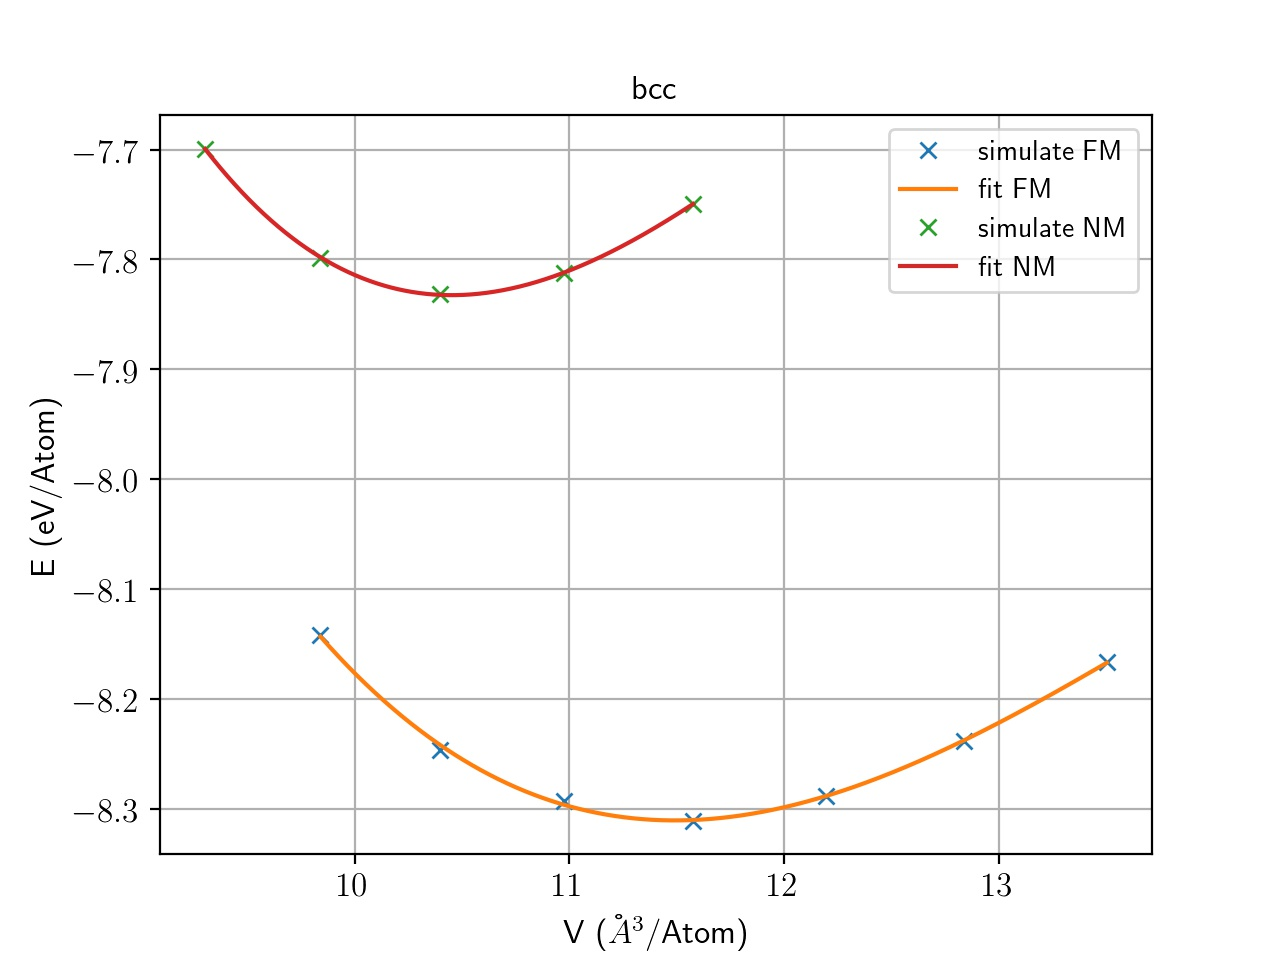
\includegraphics[width=\textwidth]{{data/q1/ev_all/bccFMNM}.jpg}
						\caption{Fe-bcc E-V}
						\label{fig:bccFMNME-V}
		 			\end{minipage}
	 				\begin{minipage}[b]{0.6\textwidth}
		 				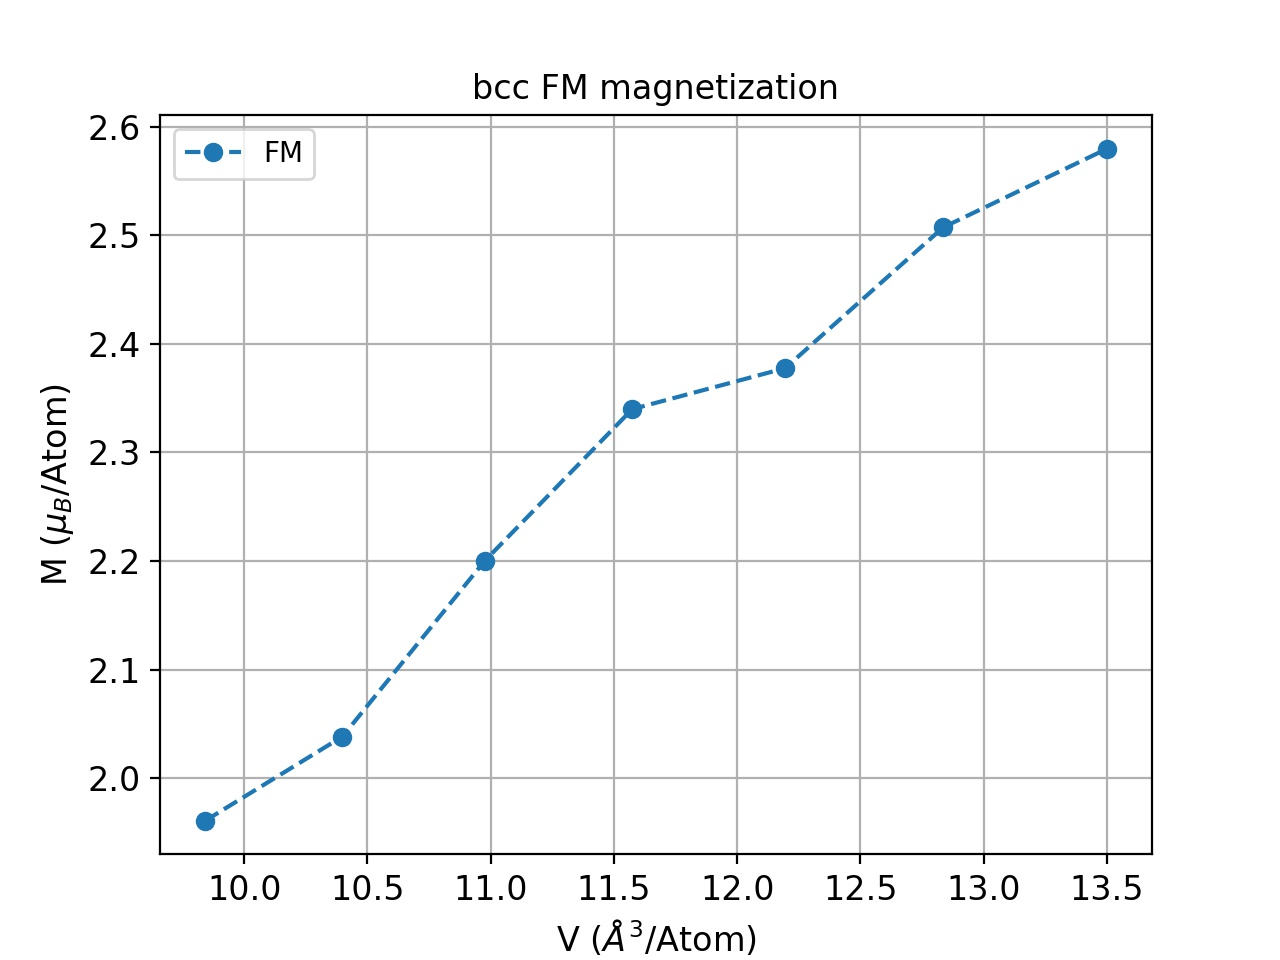
\includegraphics[width=\textwidth]{{data/q1/ev_all/bcc_M-V}.jpg}
						\caption{Fe-bcc M-V}
						\label{fig:bccMV}
		 			\end{minipage}

		 		\end{figure}
				
		 		\begin{table}[h!]
			 		\centering
			 		\begin{tabular}{c@{\hskip 0.5in}c@{\hskip 0.5in}c@{\hskip 0.5in}c} 
			 			\hline
			 			bcc & FM & NM & \\ 
			 			\hline
			 			$a_0$   & 2.84254   & 2.75474   &($\AA$)\\
			 			$B$     & 183.3448  & 278.7161  &(GPa)  \\
			 			\hline
			 		\end{tabular}
			 		\caption{bcc result from fitting with the E-V curve}
			 		\label{table:bcc}
			 	\end{table}
			 \newpage
			 
			 
		 	\item fcc
		 	
		 		\begin{figure}[h!]
		 		
			 		\begin{minipage}[b]{0.6\textwidth}
			 			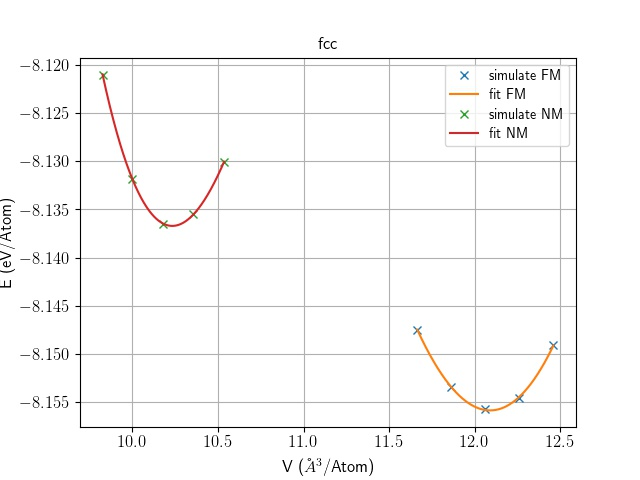
\includegraphics[width=\textwidth]{{data/q1/ev_all/fccFMNM}.jpg}
						\caption{Fe-fcc E-V}
						\label{fig:fccFMNME-V}
			 		\end{minipage}
			 		\begin{minipage}[b]{0.6\textwidth}
			 			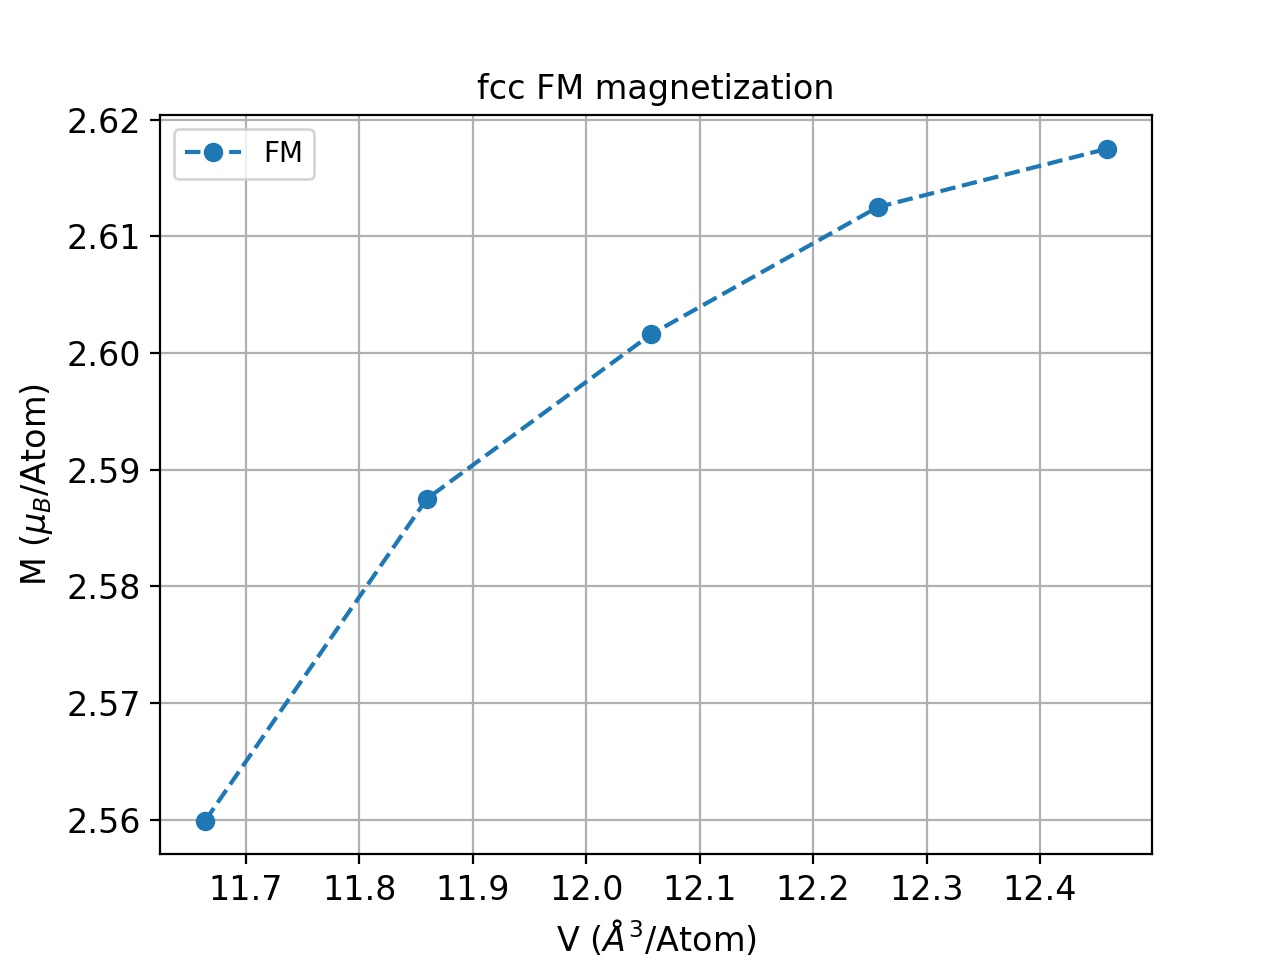
\includegraphics[width=\textwidth]{{data/q1/ev_all/fcc_M-V}.jpg}
			 			\caption{Fe-fcc M-V}
			 			\label{fig:fccMV}
			 		\end{minipage}
			 		
			 	\end{figure}

		 	
				\begin{table}[h!]
					\centering
					\begin{tabular}{c@{\hskip 0.5in}c@{\hskip 0.5in}c@{\hskip 0.5in}c} 
						\hline
						fcc & FM & NM & \\ 
						\hline
						$a_0$   & 3.64323  & 3.44638 &($\AA$)\\
						$B$     & 185.5447  & 269.3374 &(GPa)  \\
						\hline
					\end{tabular}
					\caption{fcc result from fitting with the E-V curve}
					\label{table:fcc}
				\end{table}
			\newpage
			
			
			
		 	\item hcp 
		 	
		 		The hcp is calculated with fixed $c/a$ ratio and perturb the lattice constant. Where for FM case $c/a = 1.7320$ and NM case $c/a = 1.5860$
		 		
		 		\begin{figure}[h!]
	
					\begin{minipage}[b]{0.5\textwidth}
						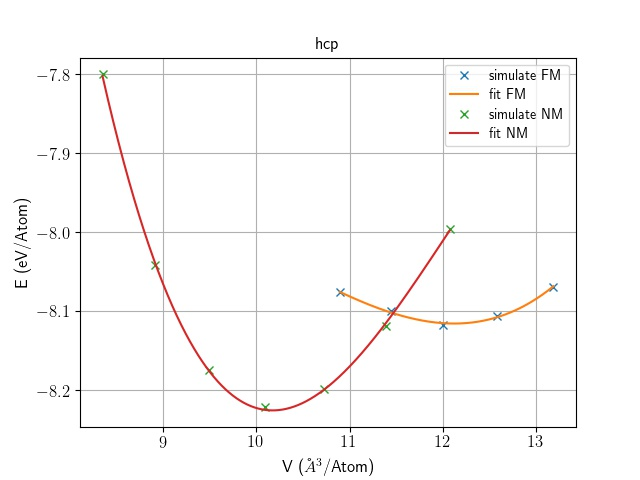
\includegraphics[width=\textwidth]{{data/q1/ev_all/hcpFMNM}.jpg}
						\caption{Fe-hcp E-V}
						\label{fig:hcpFMNME-V}
					\end{minipage}
					\begin{minipage}[b]{0.5\textwidth}
						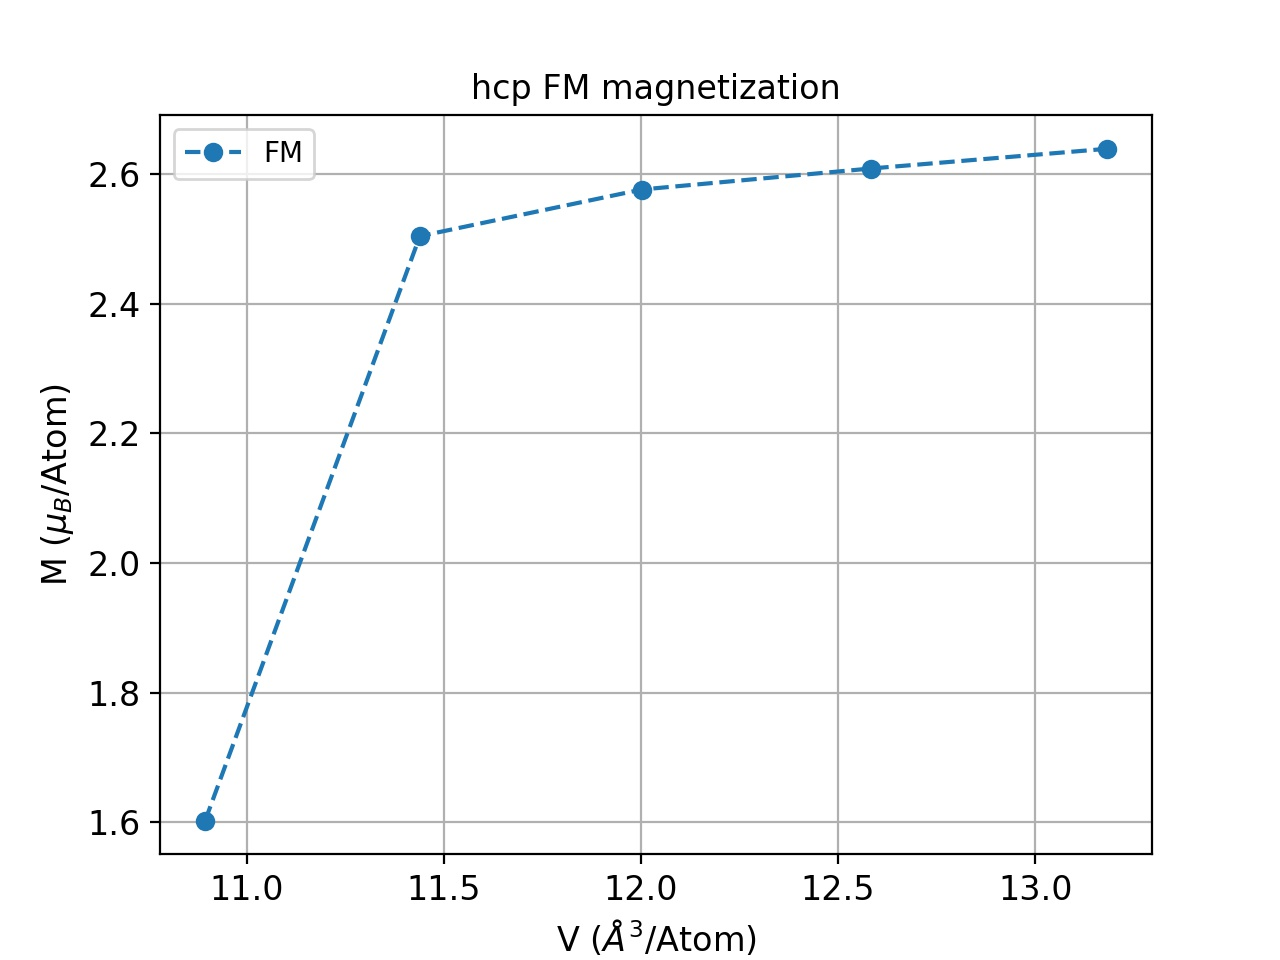
\includegraphics[width=\textwidth]{{data/q1/ev_all/hcp_M-V}.jpg}
						\caption{Fe-hcp M-V}
						\label{fig:hcpMV}
					\end{minipage}
					
				\end{figure}

				\begin{table}[h!]
					\centering
					\begin{tabular}{c@{\hskip 0.5in}c@{\hskip 0.5in}c@{\hskip 0.5in}c} 
						\hline
						hcp & FM & NM & \\ 
						\hline
						$a_0$   & 2.52821   & 2.45619 &($\AA$)\\
						$B$     & 135.1516  & 313.6009 &(GPa)  \\
						\hline
					\end{tabular}
					\caption{hcp result from fitting with the E-V curve and fixed $c/a$}
					\label{table:hcp}
				\end{table}

		 \end{itemize}
	 	\newpage
	 	 To get the transition pressure from ferro-magnetic bcc to non-magnetic hcp, we use the relation for pressure $P$:
	 	 \begin{align}
	 	 	P = -\frac{\partial E}{\partial V}
	 	 \end{align} 
	 	 
	 	 this suggest that the transition happened when the E-V curves for bcc and hcp have the same slopes. following shows the E-V plot and P-V plot for FM-bcc and NM-hcp Fe.
	 	 
	 	 \begin{figure}[h!]
	 	 	
	 	 	\begin{minipage}[b]{0.5\textwidth}
	 	 		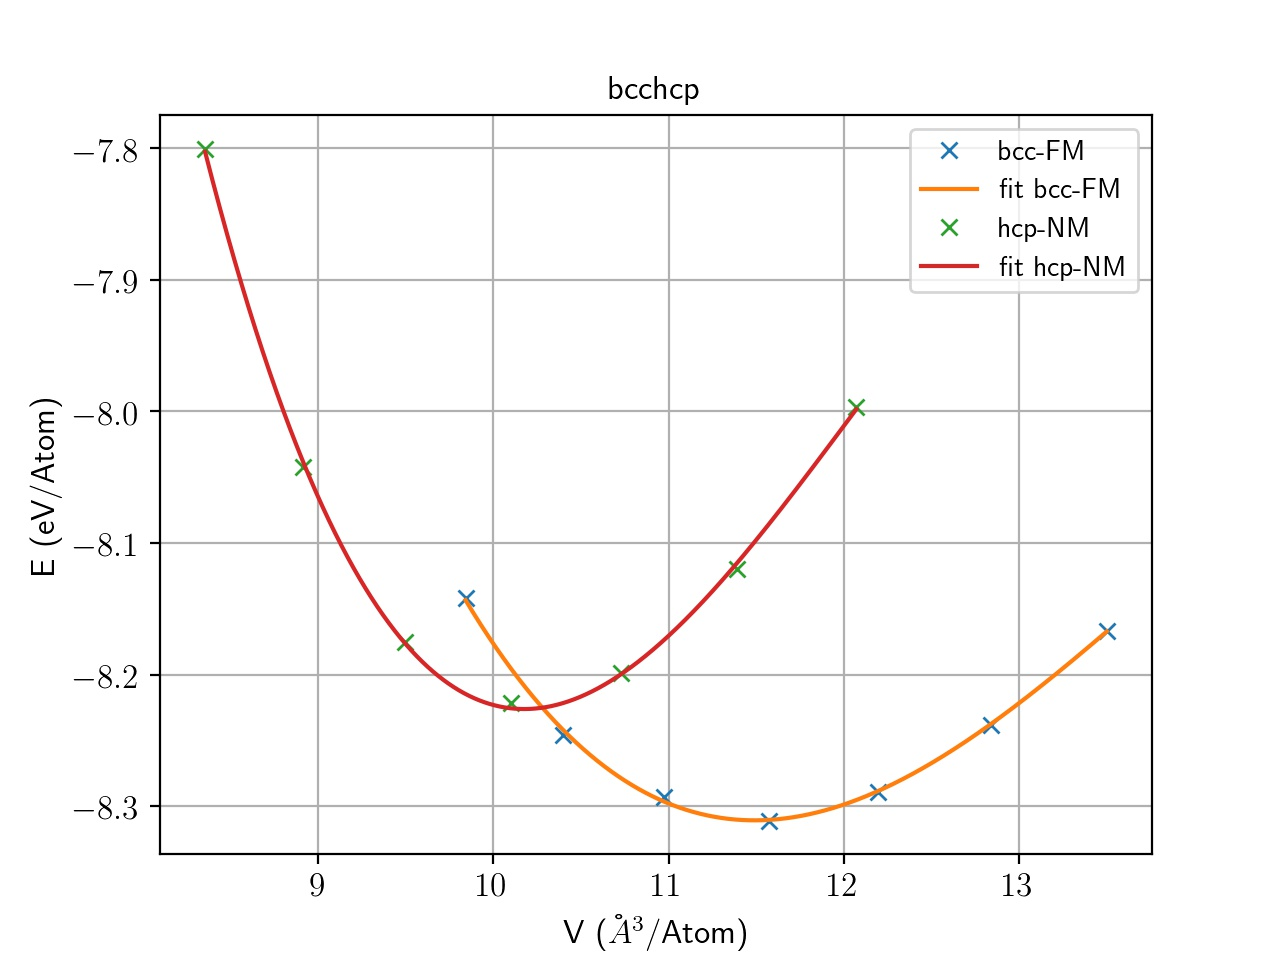
\includegraphics[width=\textwidth]{{data/q1/ev_all/bcchcpFMNM}.jpg}
	 	 		\caption{FM-bcc and NM-hcp E-V}
	 	 		\label{fig:bcchcpFMNME-V}
	 	 	\end{minipage}
	 	 	\begin{minipage}[b]{0.5\textwidth}
	 	 		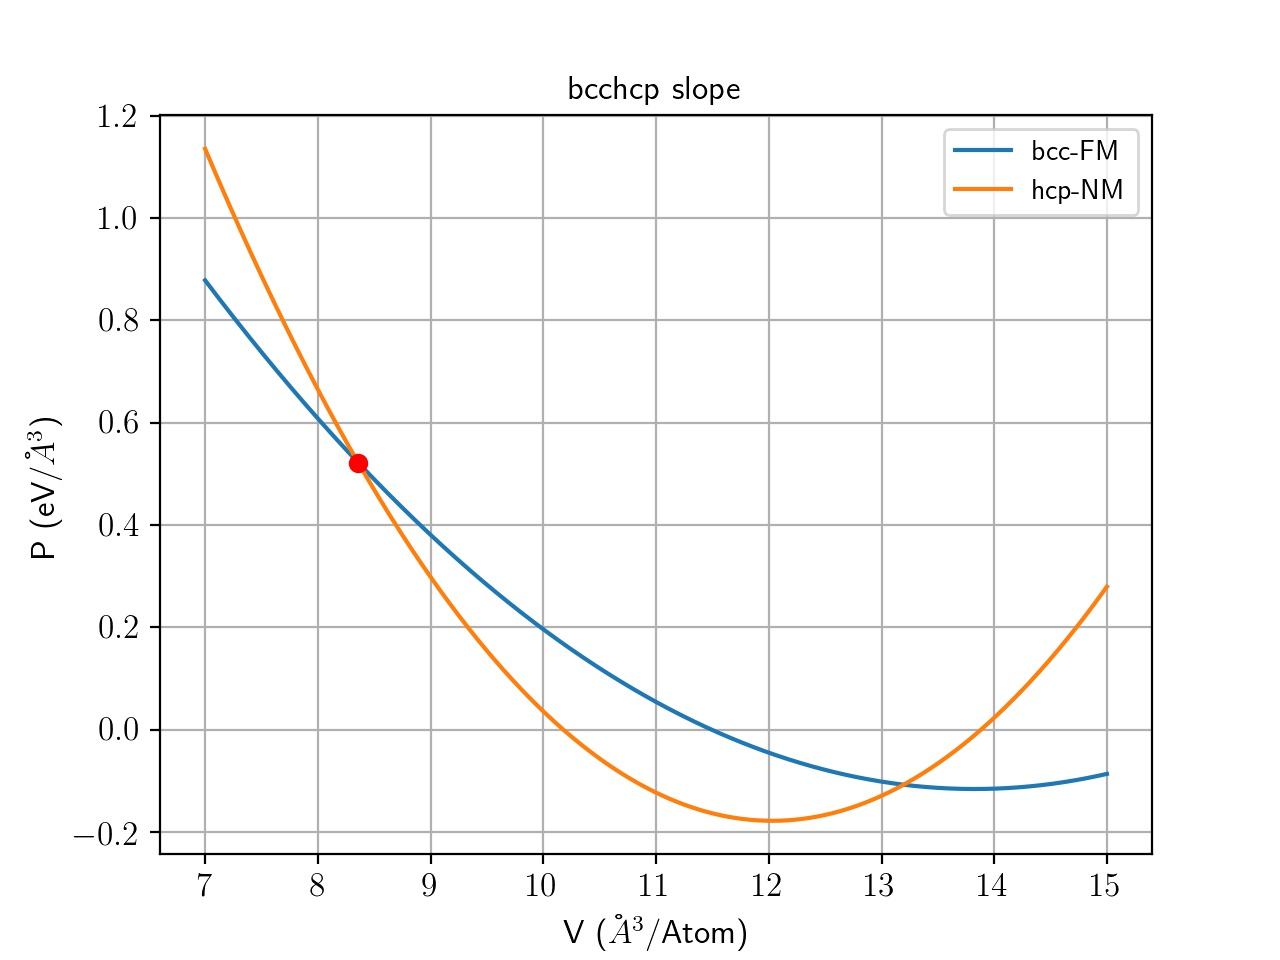
\includegraphics[width=\textwidth]{{data/q1/ev_all/bcchcpP-V}.jpg}
	 	 		\caption{FM-bcc and NM-hcp P-V}
	 	 		\label{fig:bcchcpPV}
	 	 	\end{minipage}
	 	 	
	 	 \end{figure} 
	 	 
	 	 where we find the transition pressure is :
	 	 \begin{align}
	 	 	P_c &= 0.522093 (eV/\AA^3) \\
	 	 	    &= 83.53488 (GPa)
	 	 \end{align}
	 	 \newpage
	 	 \item Finally we list all the calculation results in below:
	 	  
		 \begin{table}[h!]
			\centering
			\begin{tabular}{c@{\hskip 0.5in}c@{\hskip 0.5in}c@{\hskip 0.5in}c} 
				\hline
				bcc & FM & NM & \\ 
				\hline
				$a_0$   & 2.84254   & 2.75474   &($\AA$)\\
				$V_0$   & 11.4839  & 10.4523 &($\AA^3/Atom$)\\
				$B$     & 183.3448  & 278.7161  &(GPa)  \\
				$M$     & 2.3312  & -- & ($\mu_B/Atom$) \\
				\hline
			\end{tabular}
			\label{table:bccall}
		\end{table}	 
	
		\begin{table}[h!]
			\centering
			\begin{tabular}{c@{\hskip 0.5in}c@{\hskip 0.5in}c@{\hskip 0.5in}c} 
				\hline
				fcc & FM & NM & \\ 
				\hline
				$a_0$   & 3.64323  & 3.44638 &($\AA$)\\
				$V_0$   & 12.0893 & 10.2336 &($\AA^3/Atom$)\\
				$B$     & 185.5447  & 269.3374 &(GPa)  \\
				$M$     & 2.6052  & -- & ($\mu_B/Atom$) \\
				\hline
			\end{tabular}
			\label{table:fccall}
		\end{table}
	
		\begin{table}[h!]
			\centering
			\begin{tabular}{c@{\hskip 0.5in}c@{\hskip 0.5in}c@{\hskip 0.5in}c} 
				\hline
				hcp & FM & NM & \\ 
				\hline
				$a_0$   & 2.52821   & 2.45619 &($\AA$)\\
				$c/a$   & 1.7320   & 1.5860 &\\
				$V_0$   & 12.1191  & 10.1763 &($\AA^3/Atom$)\\
				$B$     & 135.1516  & 313.6009 &(GPa)  \\
				$M$     & 2.58355  & -- & ($\mu_B/Atom$) \\
				\hline
			\end{tabular}
			\label{table:hcpall}
		\end{table}
	
	\end{enumerate} 
	\clearpage
	
	%q2:
	\item 
	\begin{enumerate}[label=(\alph*)]
		\item The calculation results of fcc-Au and diamond-Si without spin-orbital coupling. 
		\begin{itemize}
			\item Au
			
				Following shows the bands structure, density of state for Au without spin orbital coupling(non-relativistic). The calculation of band structure are consist with previous study \cite{JoPAu} and the DOS consist with bulk DOS in \cite{photonics2020659}. 
				 
			 	\begin{figure}[h!]
				
					\begin{minipage}[b]{0.45\textwidth}
						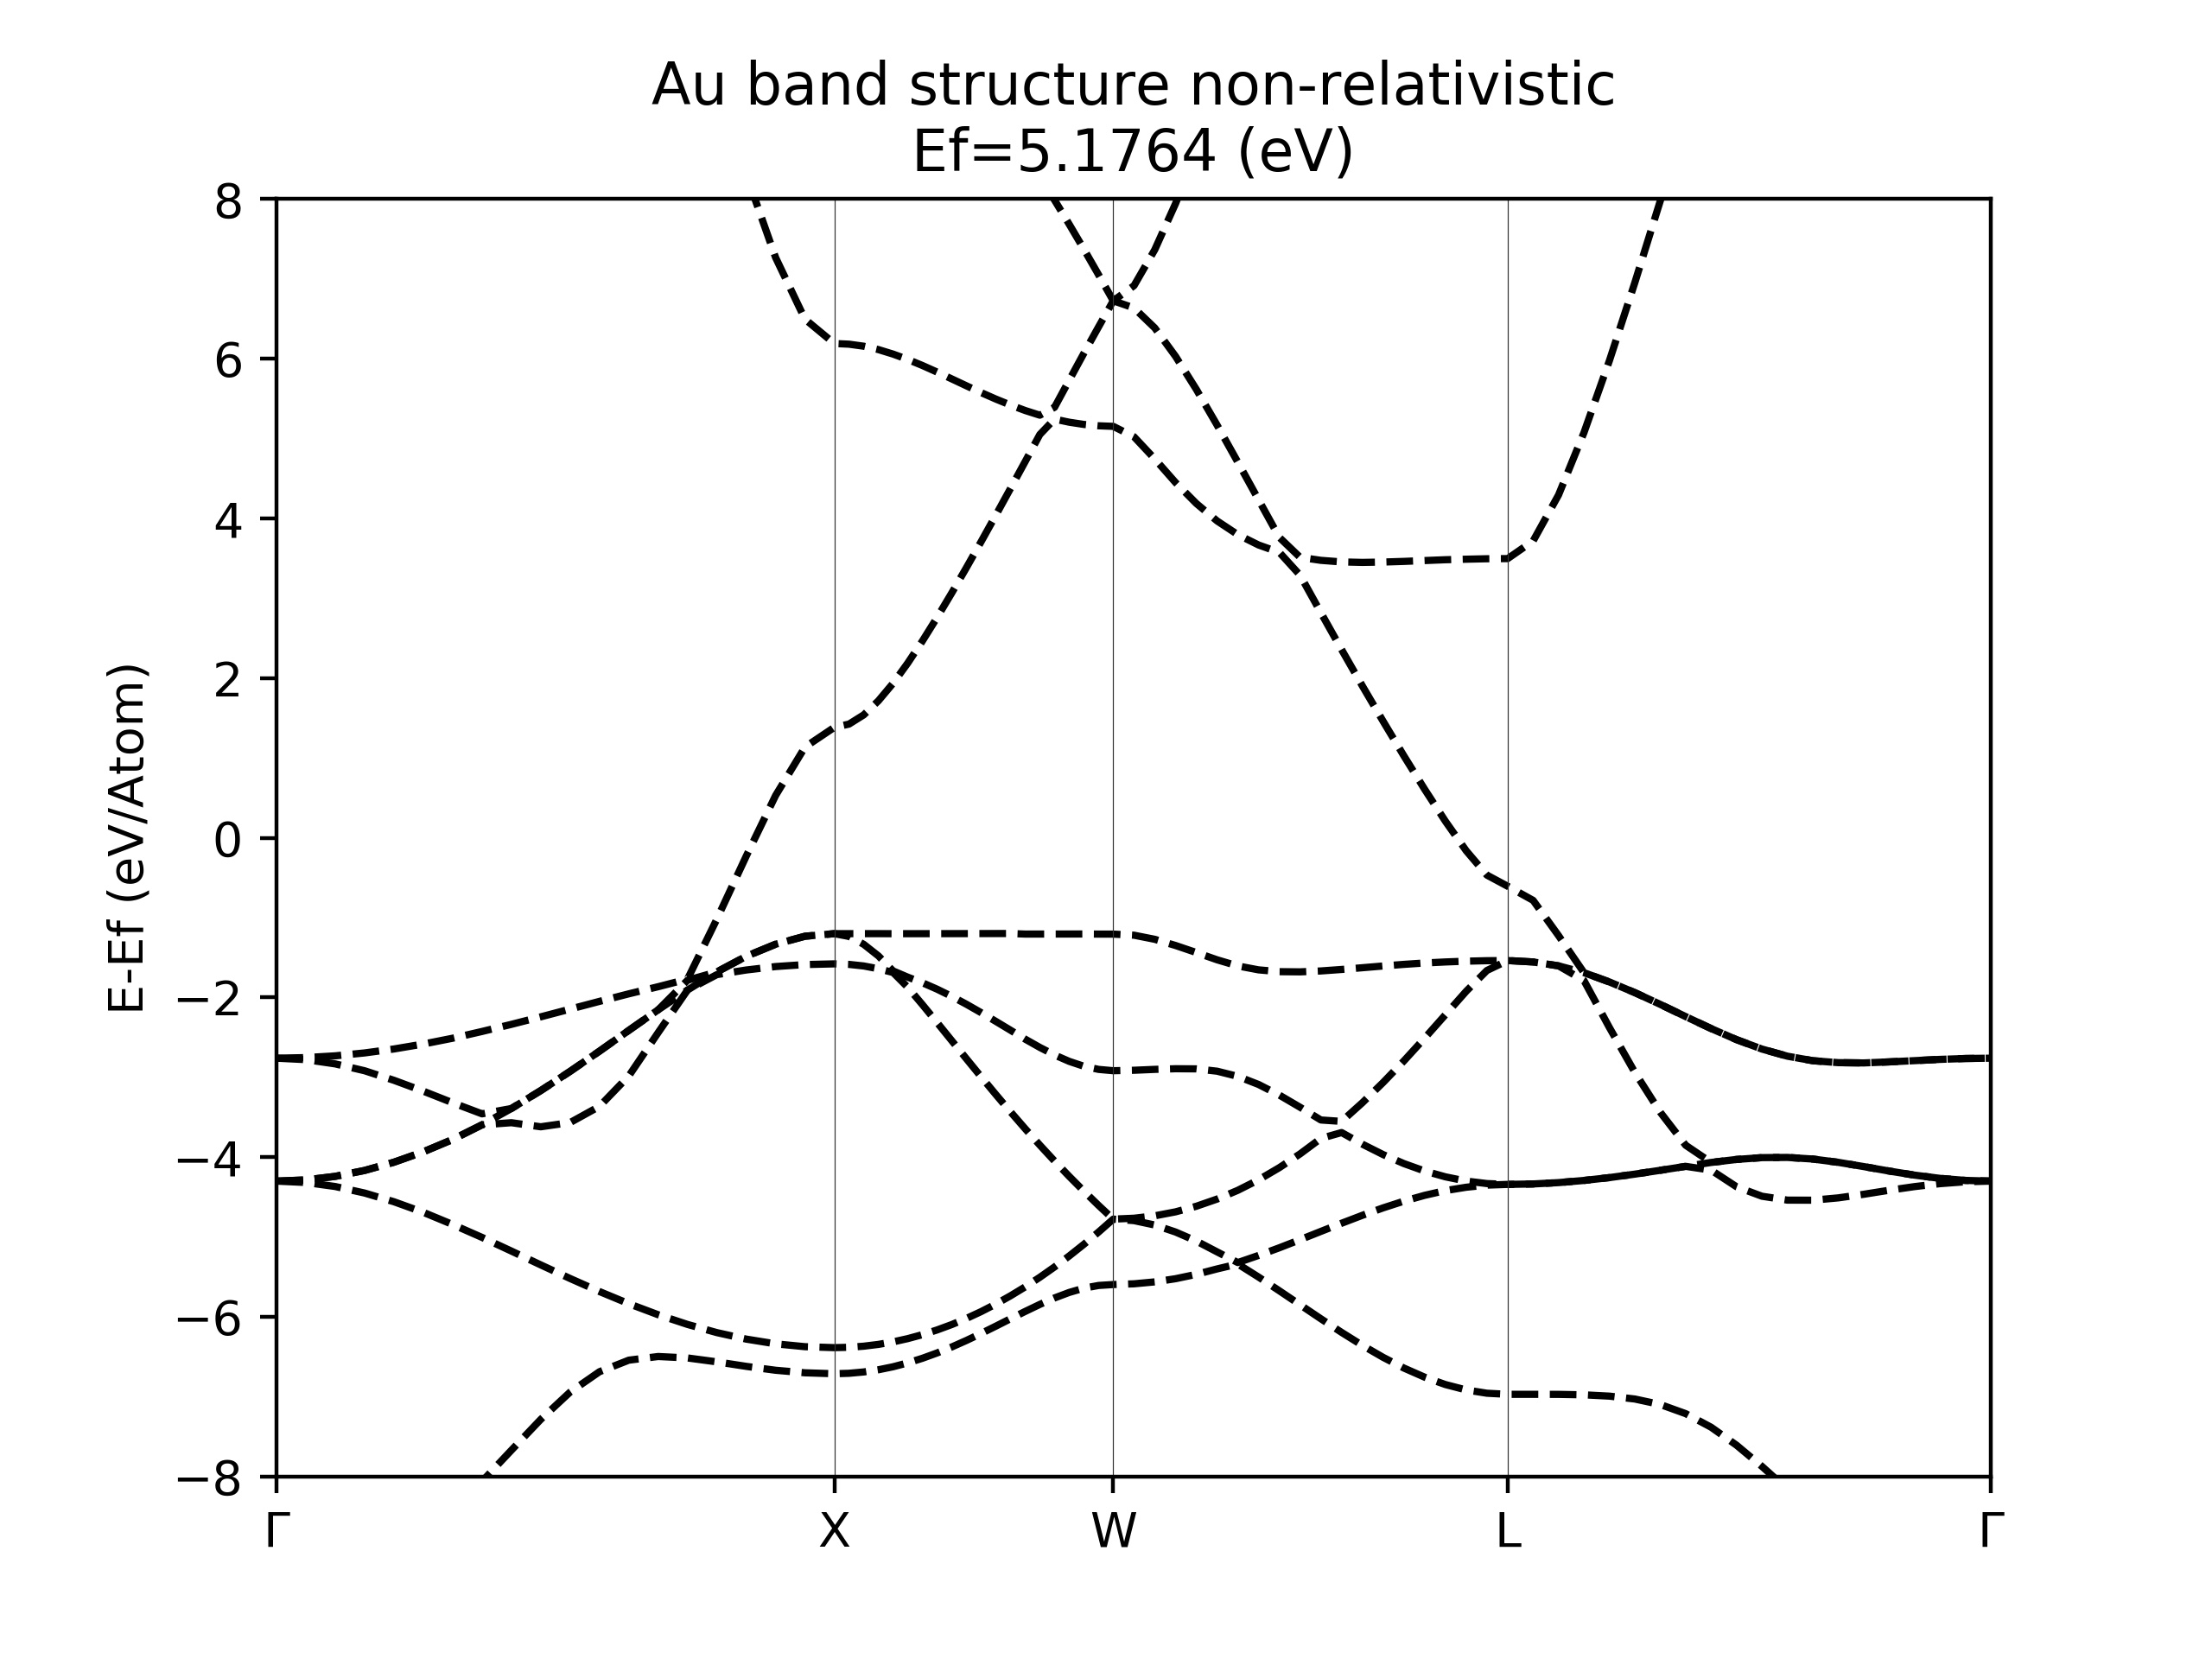
\includegraphics[width=\textwidth]{{data/q2/All_Data/Au_data/Au}.jpg}
						\caption{Au band structure}
						\label{fig:Auband}
					\end{minipage}
					\begin{minipage}[b]{0.45\textwidth}
						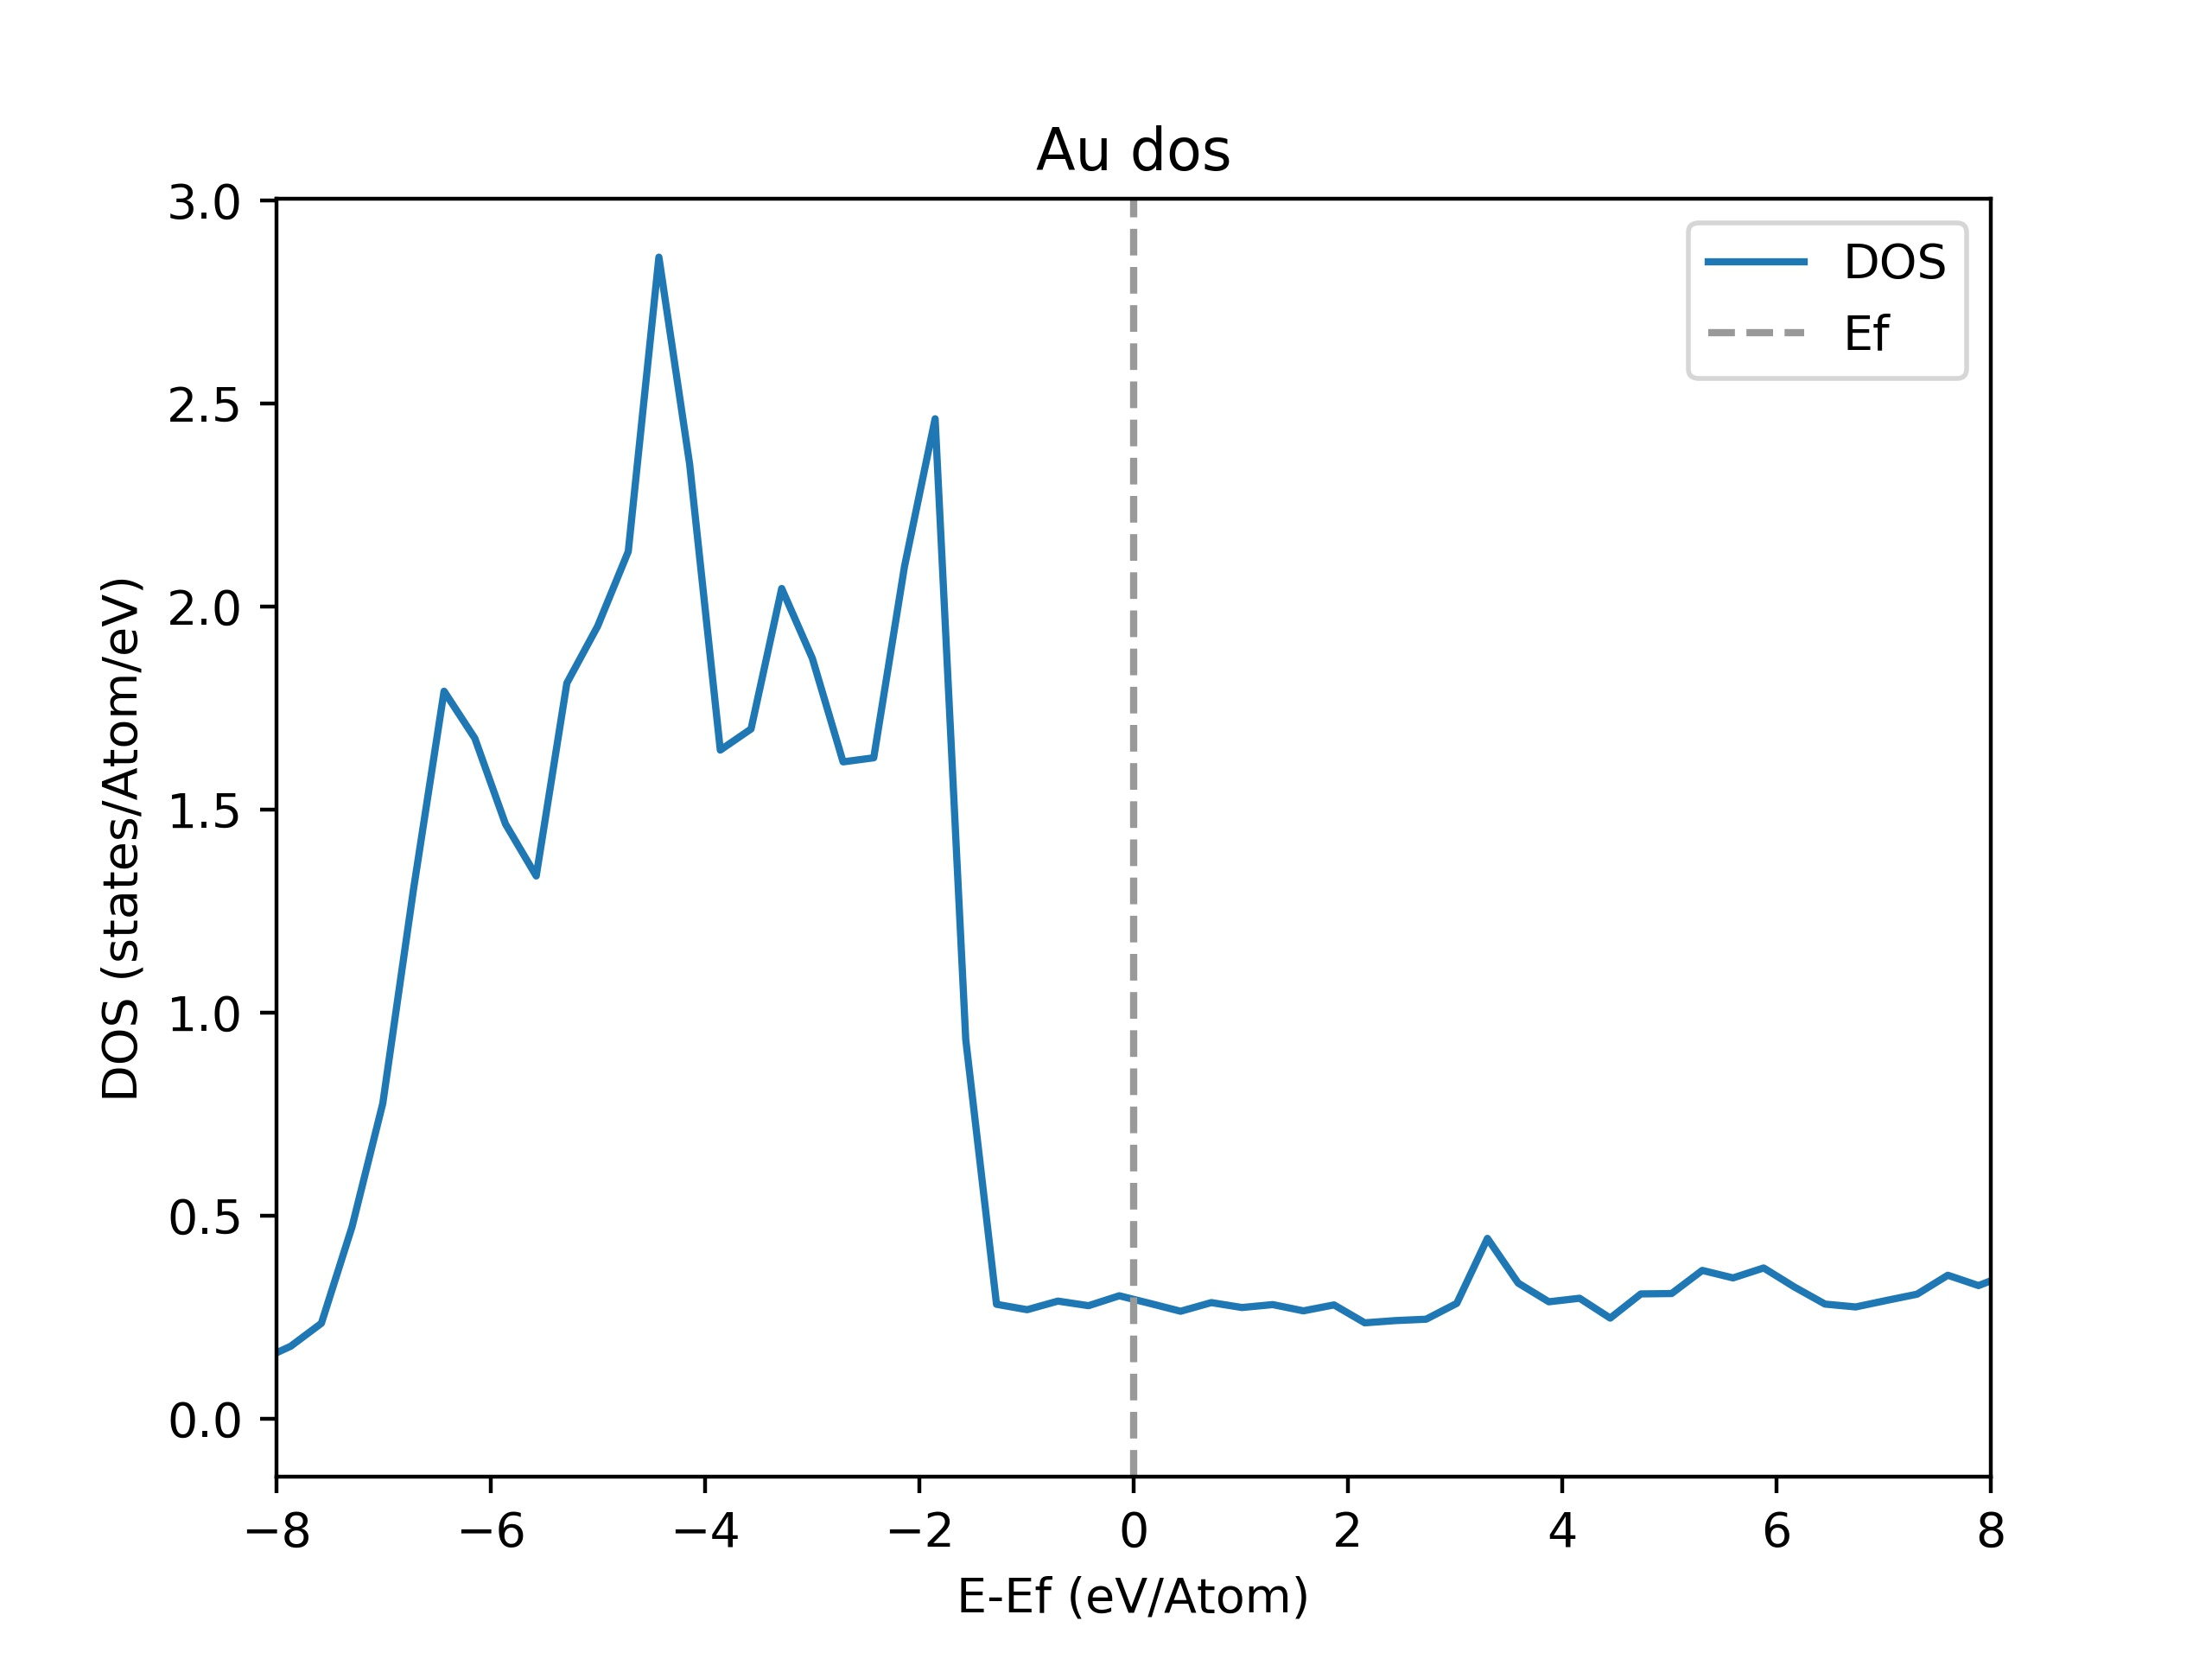
\includegraphics[width=\textwidth]{{data/q2/All_Data/Au_data/Au_dos}.jpg}
						\caption{Au DOS}
						\label{fig:Audos}
					\end{minipage}
					\begin{minipage}[b]{0.45\textwidth}
						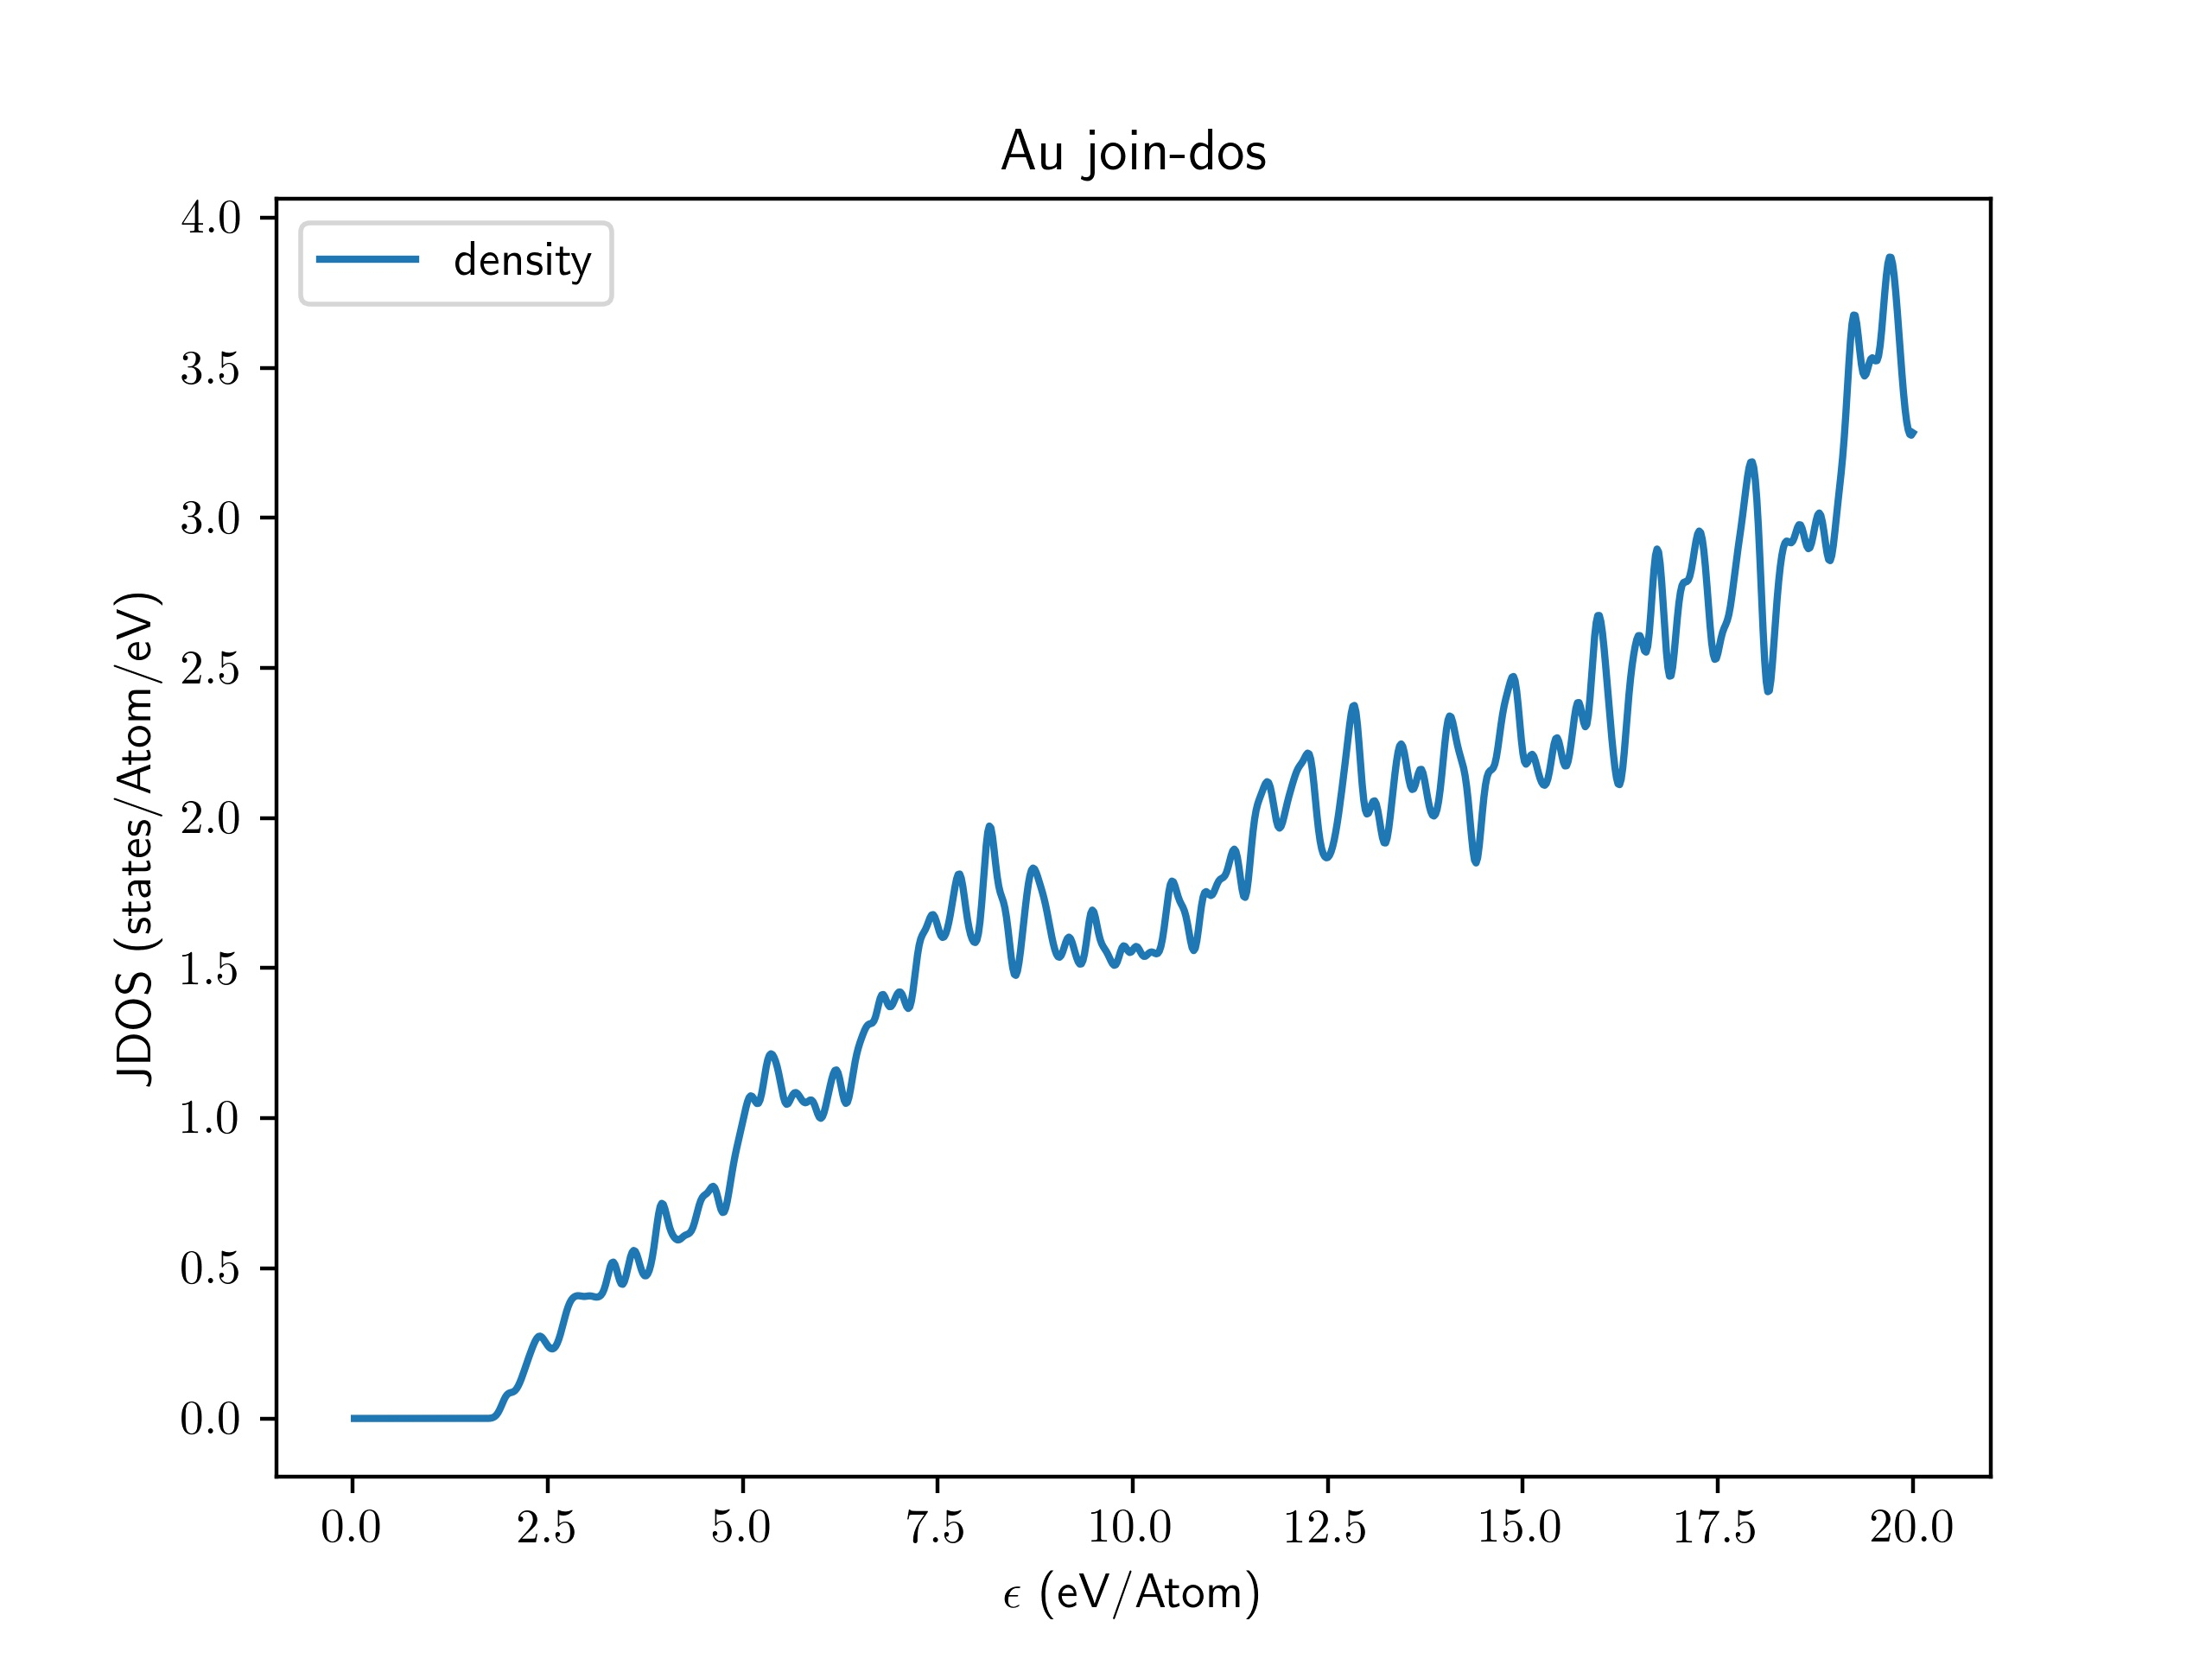
\includegraphics[width=\textwidth]{{data/q2/All_Data/Au_data/Au_jdos}.jpg}
						\caption{Au join-DOS}
						\label{fig:Aujdos}
					\end{minipage}
					\begin{minipage}[b]{0.45\textwidth}
						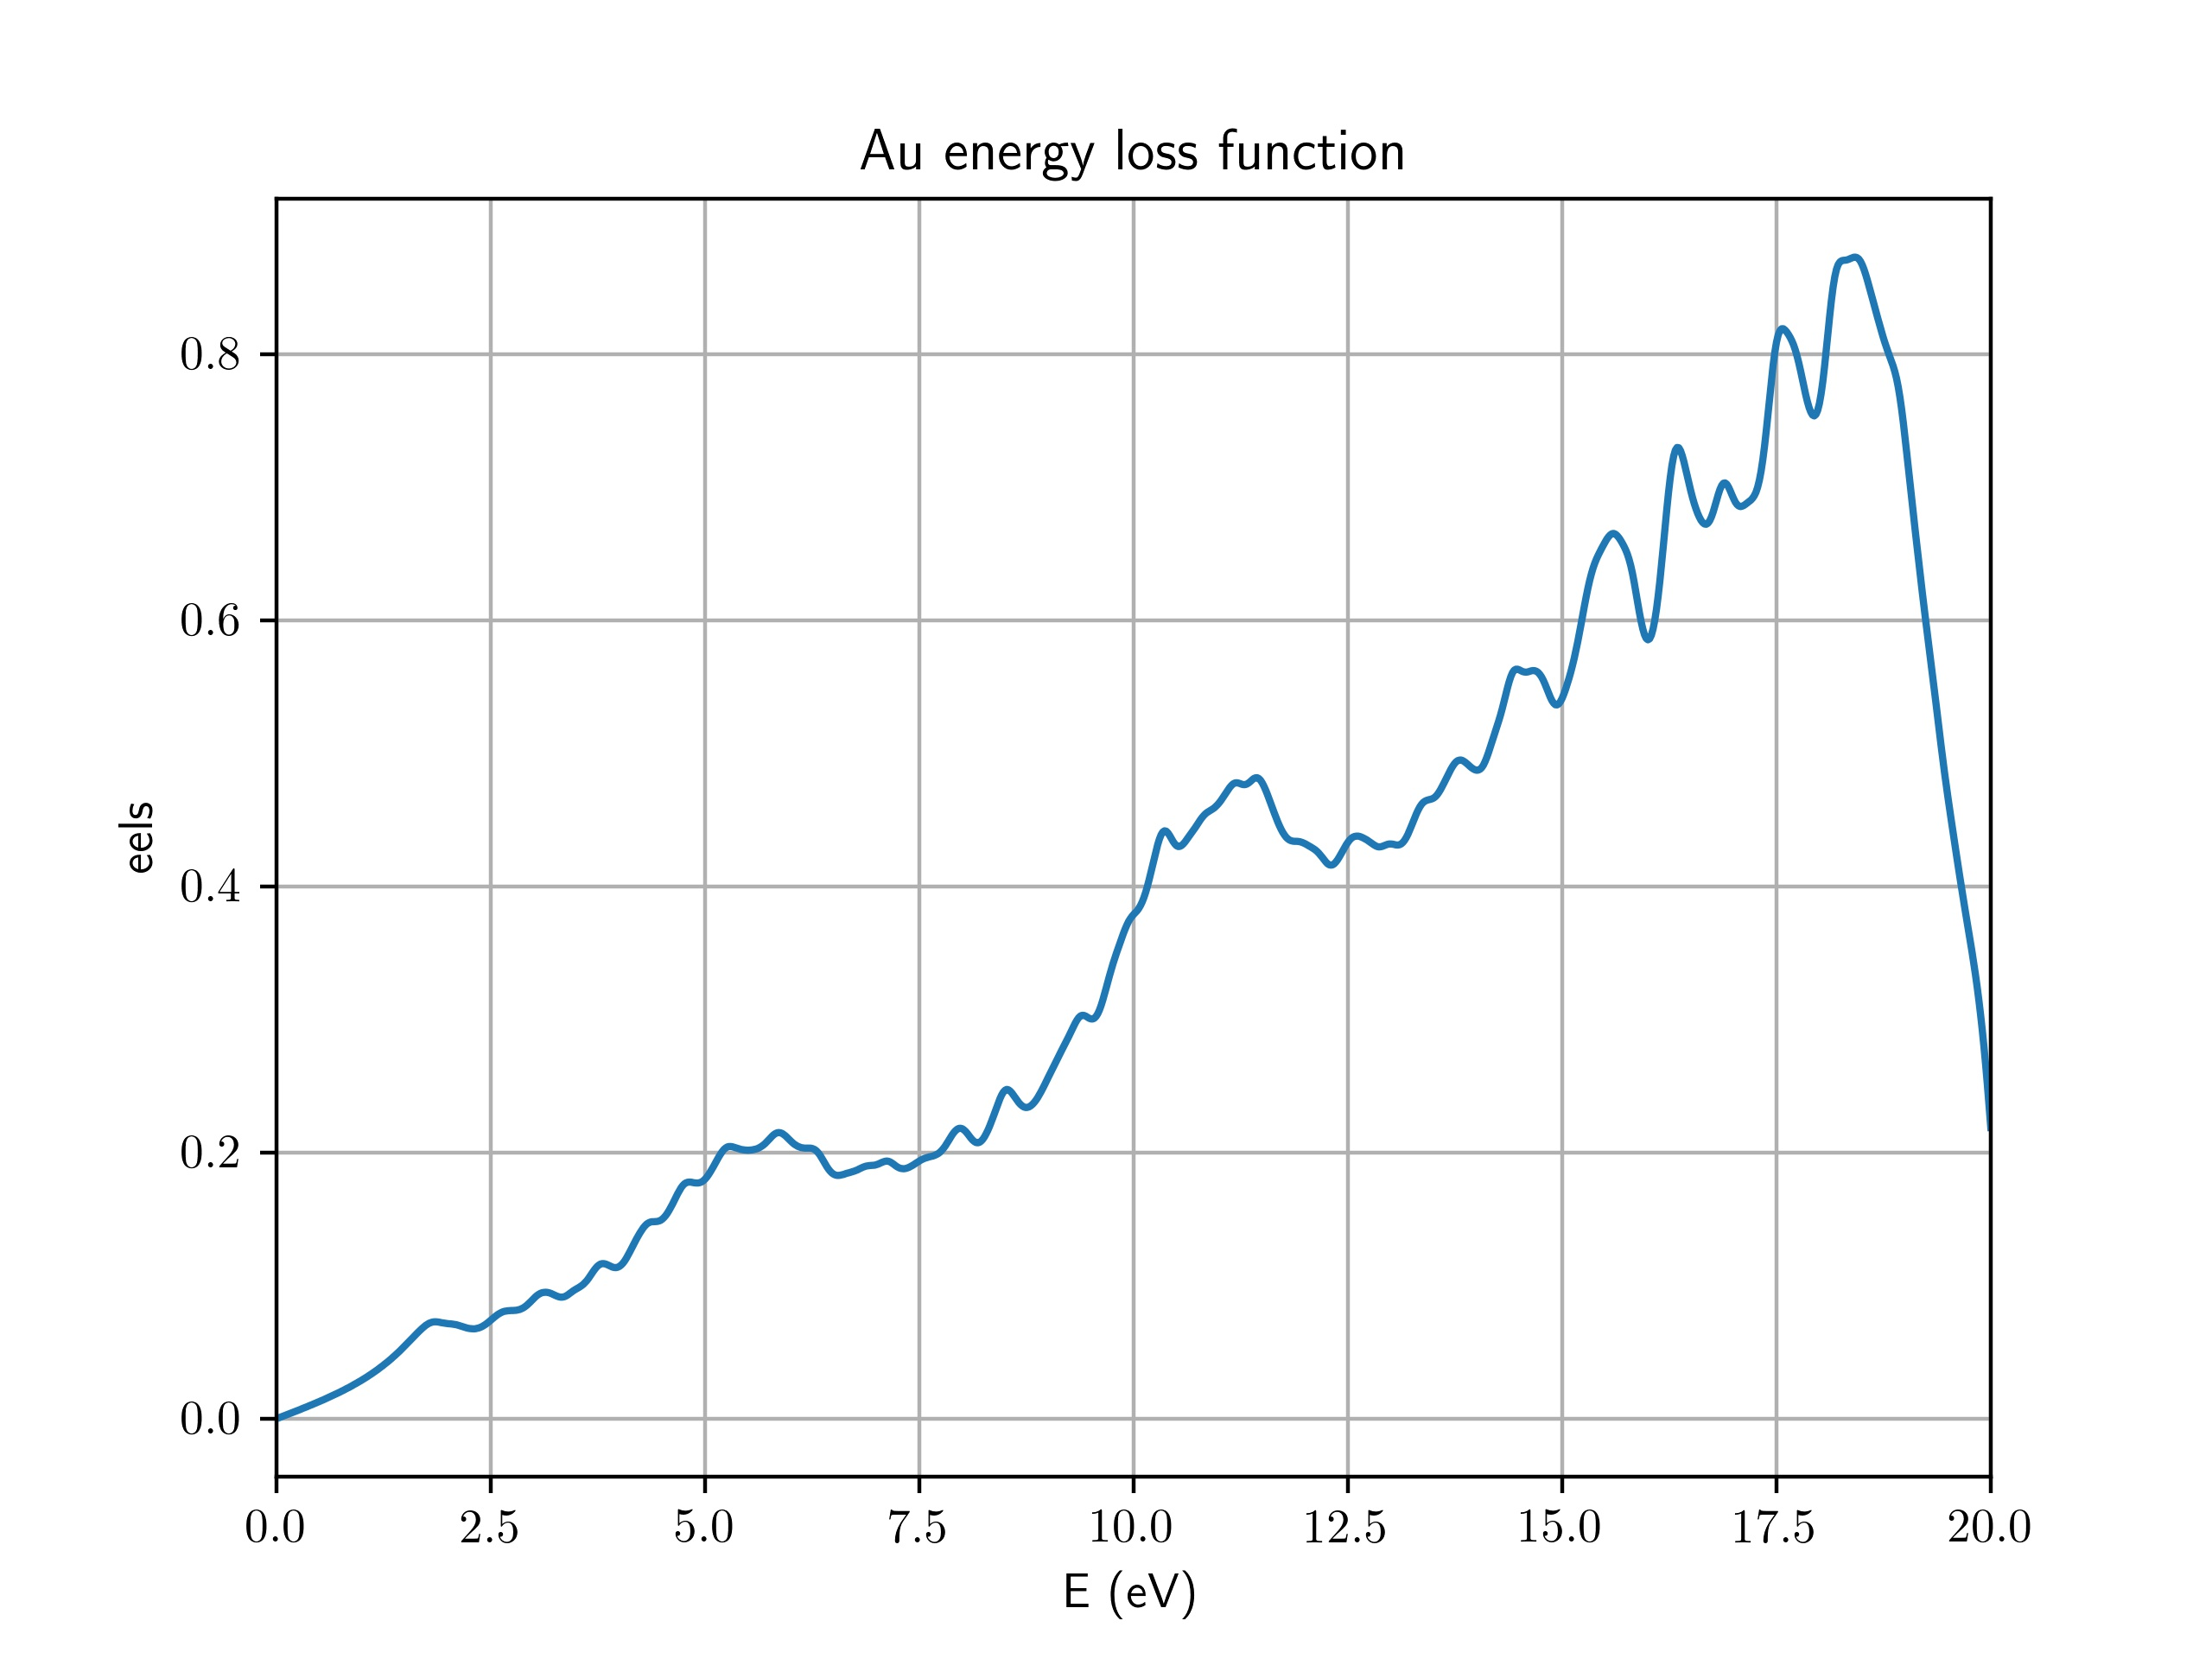
\includegraphics[width=\textwidth]{{data/q2/All_Data/Au_data/Au_eels}.jpg}
						\caption{Au energy loss function}
						\label{fig:Aueels}
					\end{minipage}
				\end{figure}
				\begin{figure}[h!]
					\begin{minipage}[b]{0.45\textwidth}
						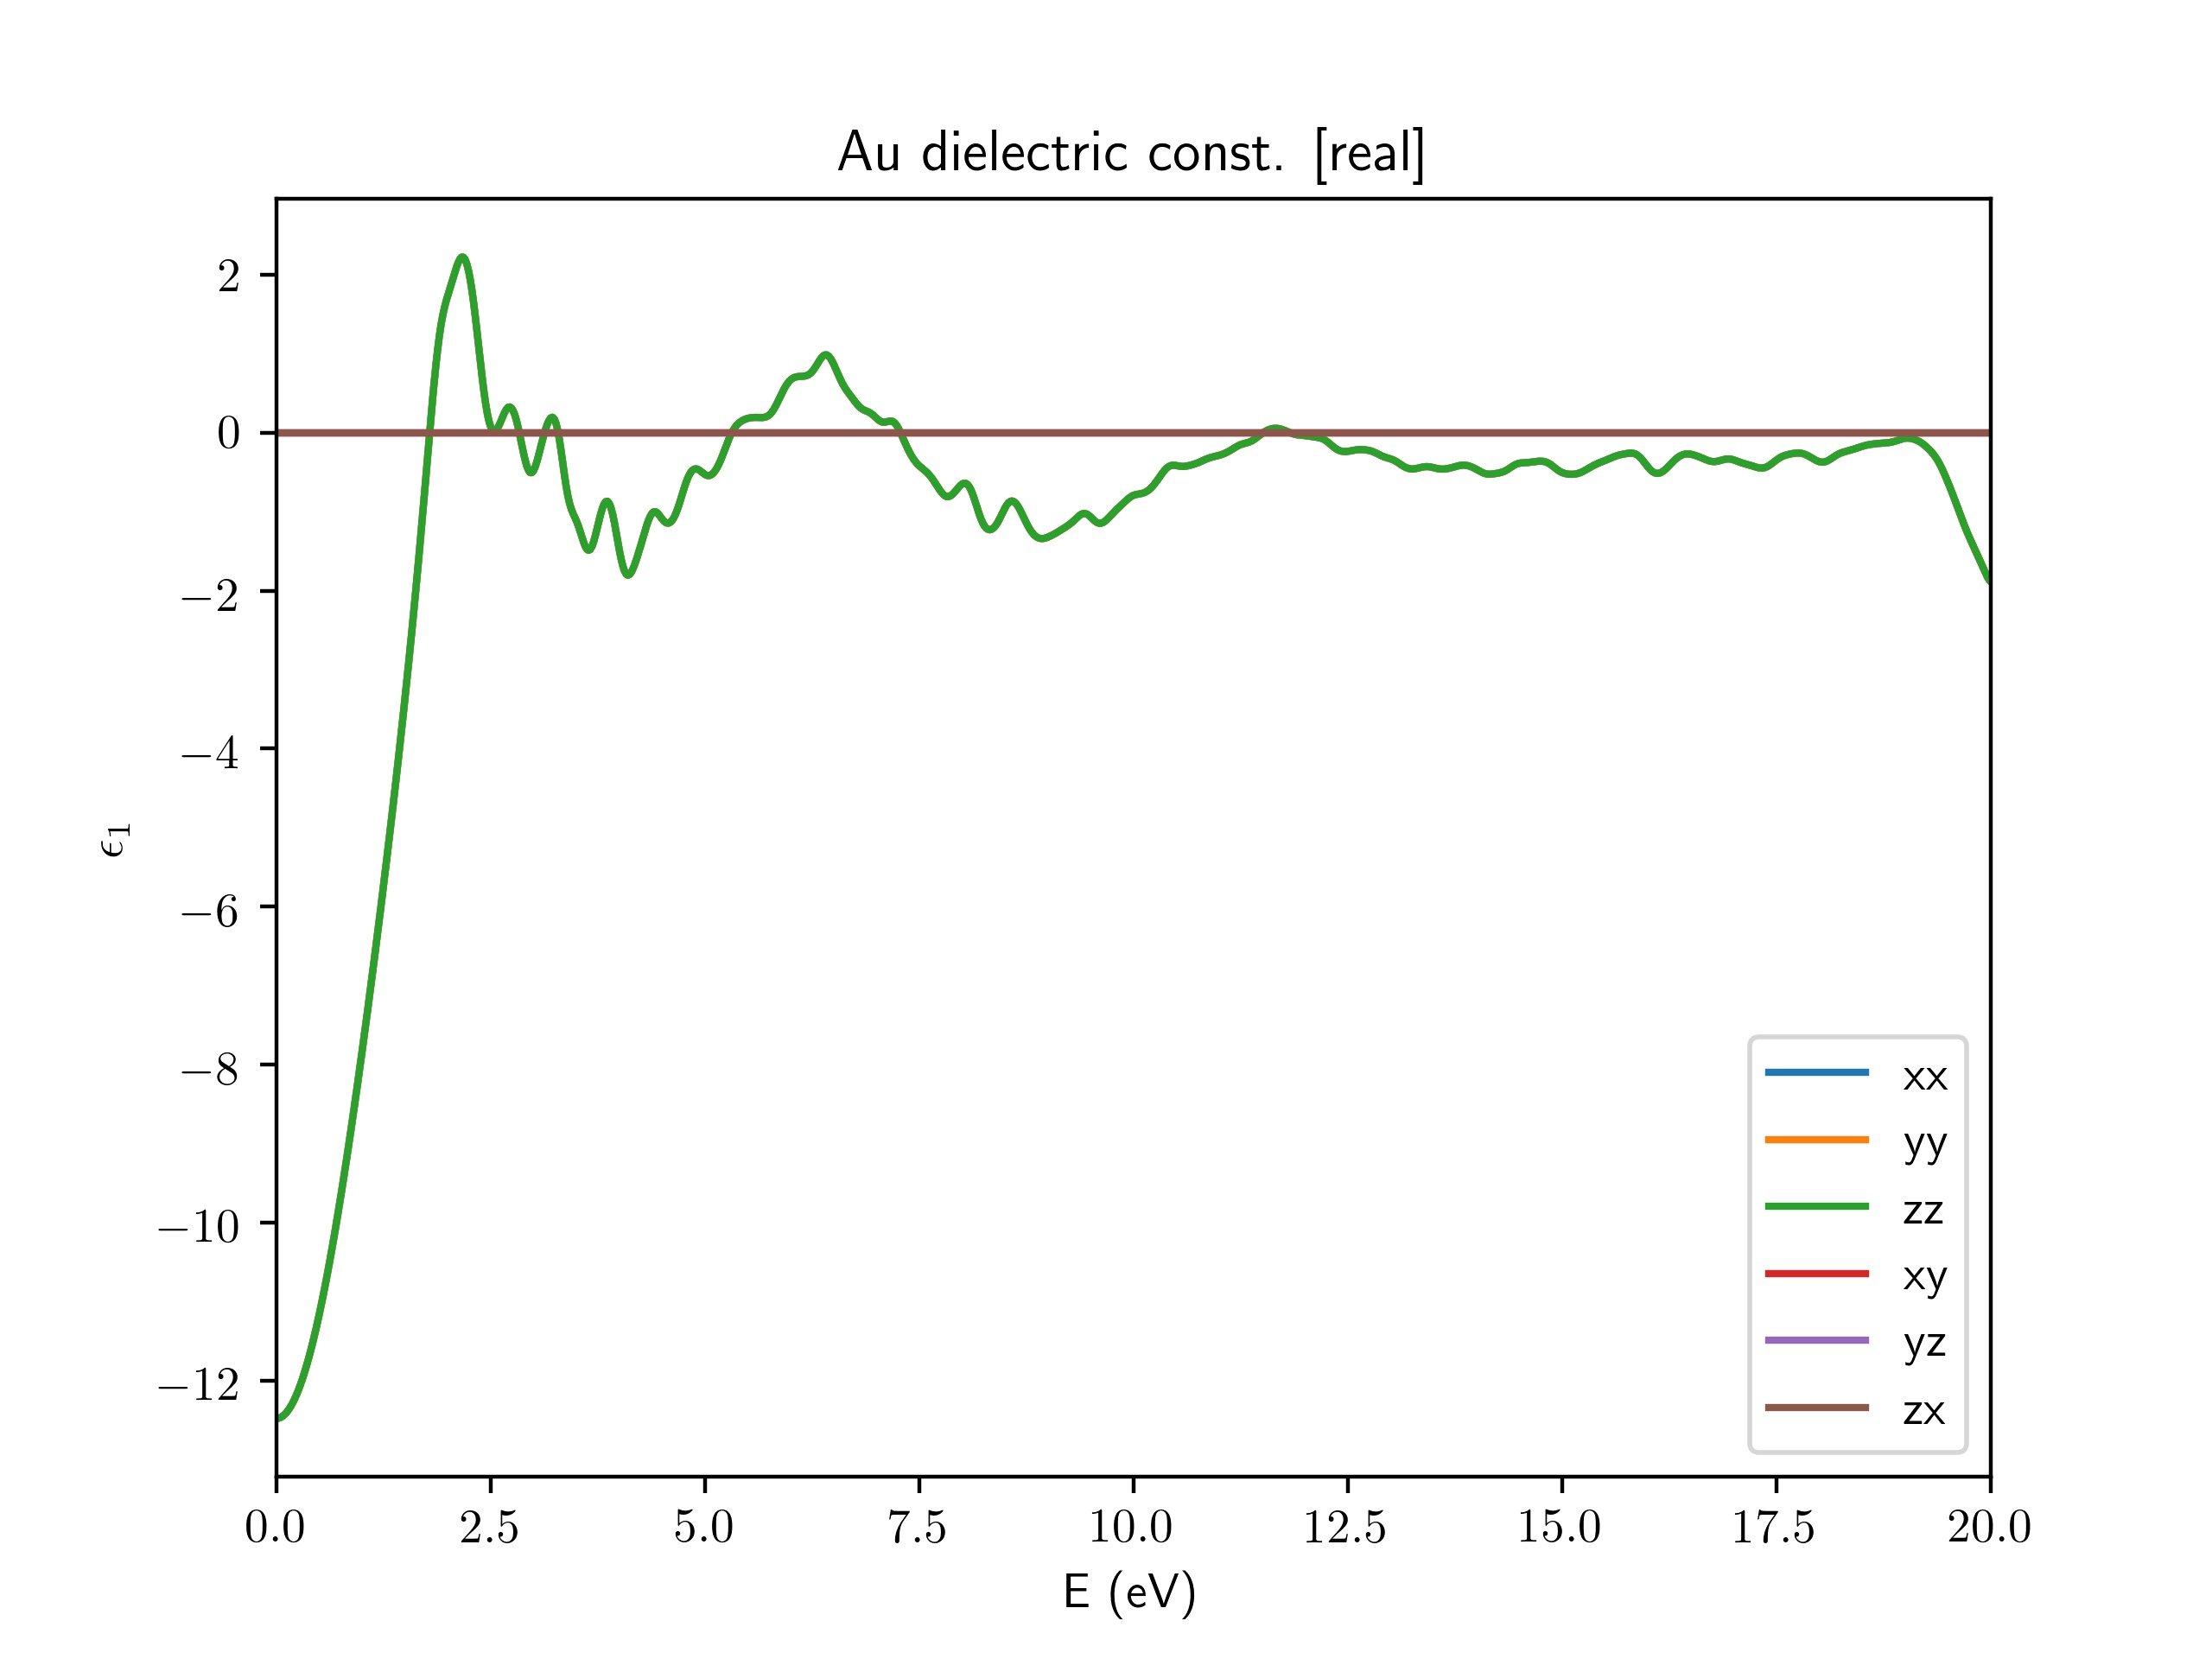
\includegraphics[width=\textwidth]{{data/q2/All_Data/Au_data/Au_epsre}.jpg}
						\caption{Au dielectric constant (real)}
						\label{fig:Auepsre}
					\end{minipage}
					\begin{minipage}[b]{0.45\textwidth}
						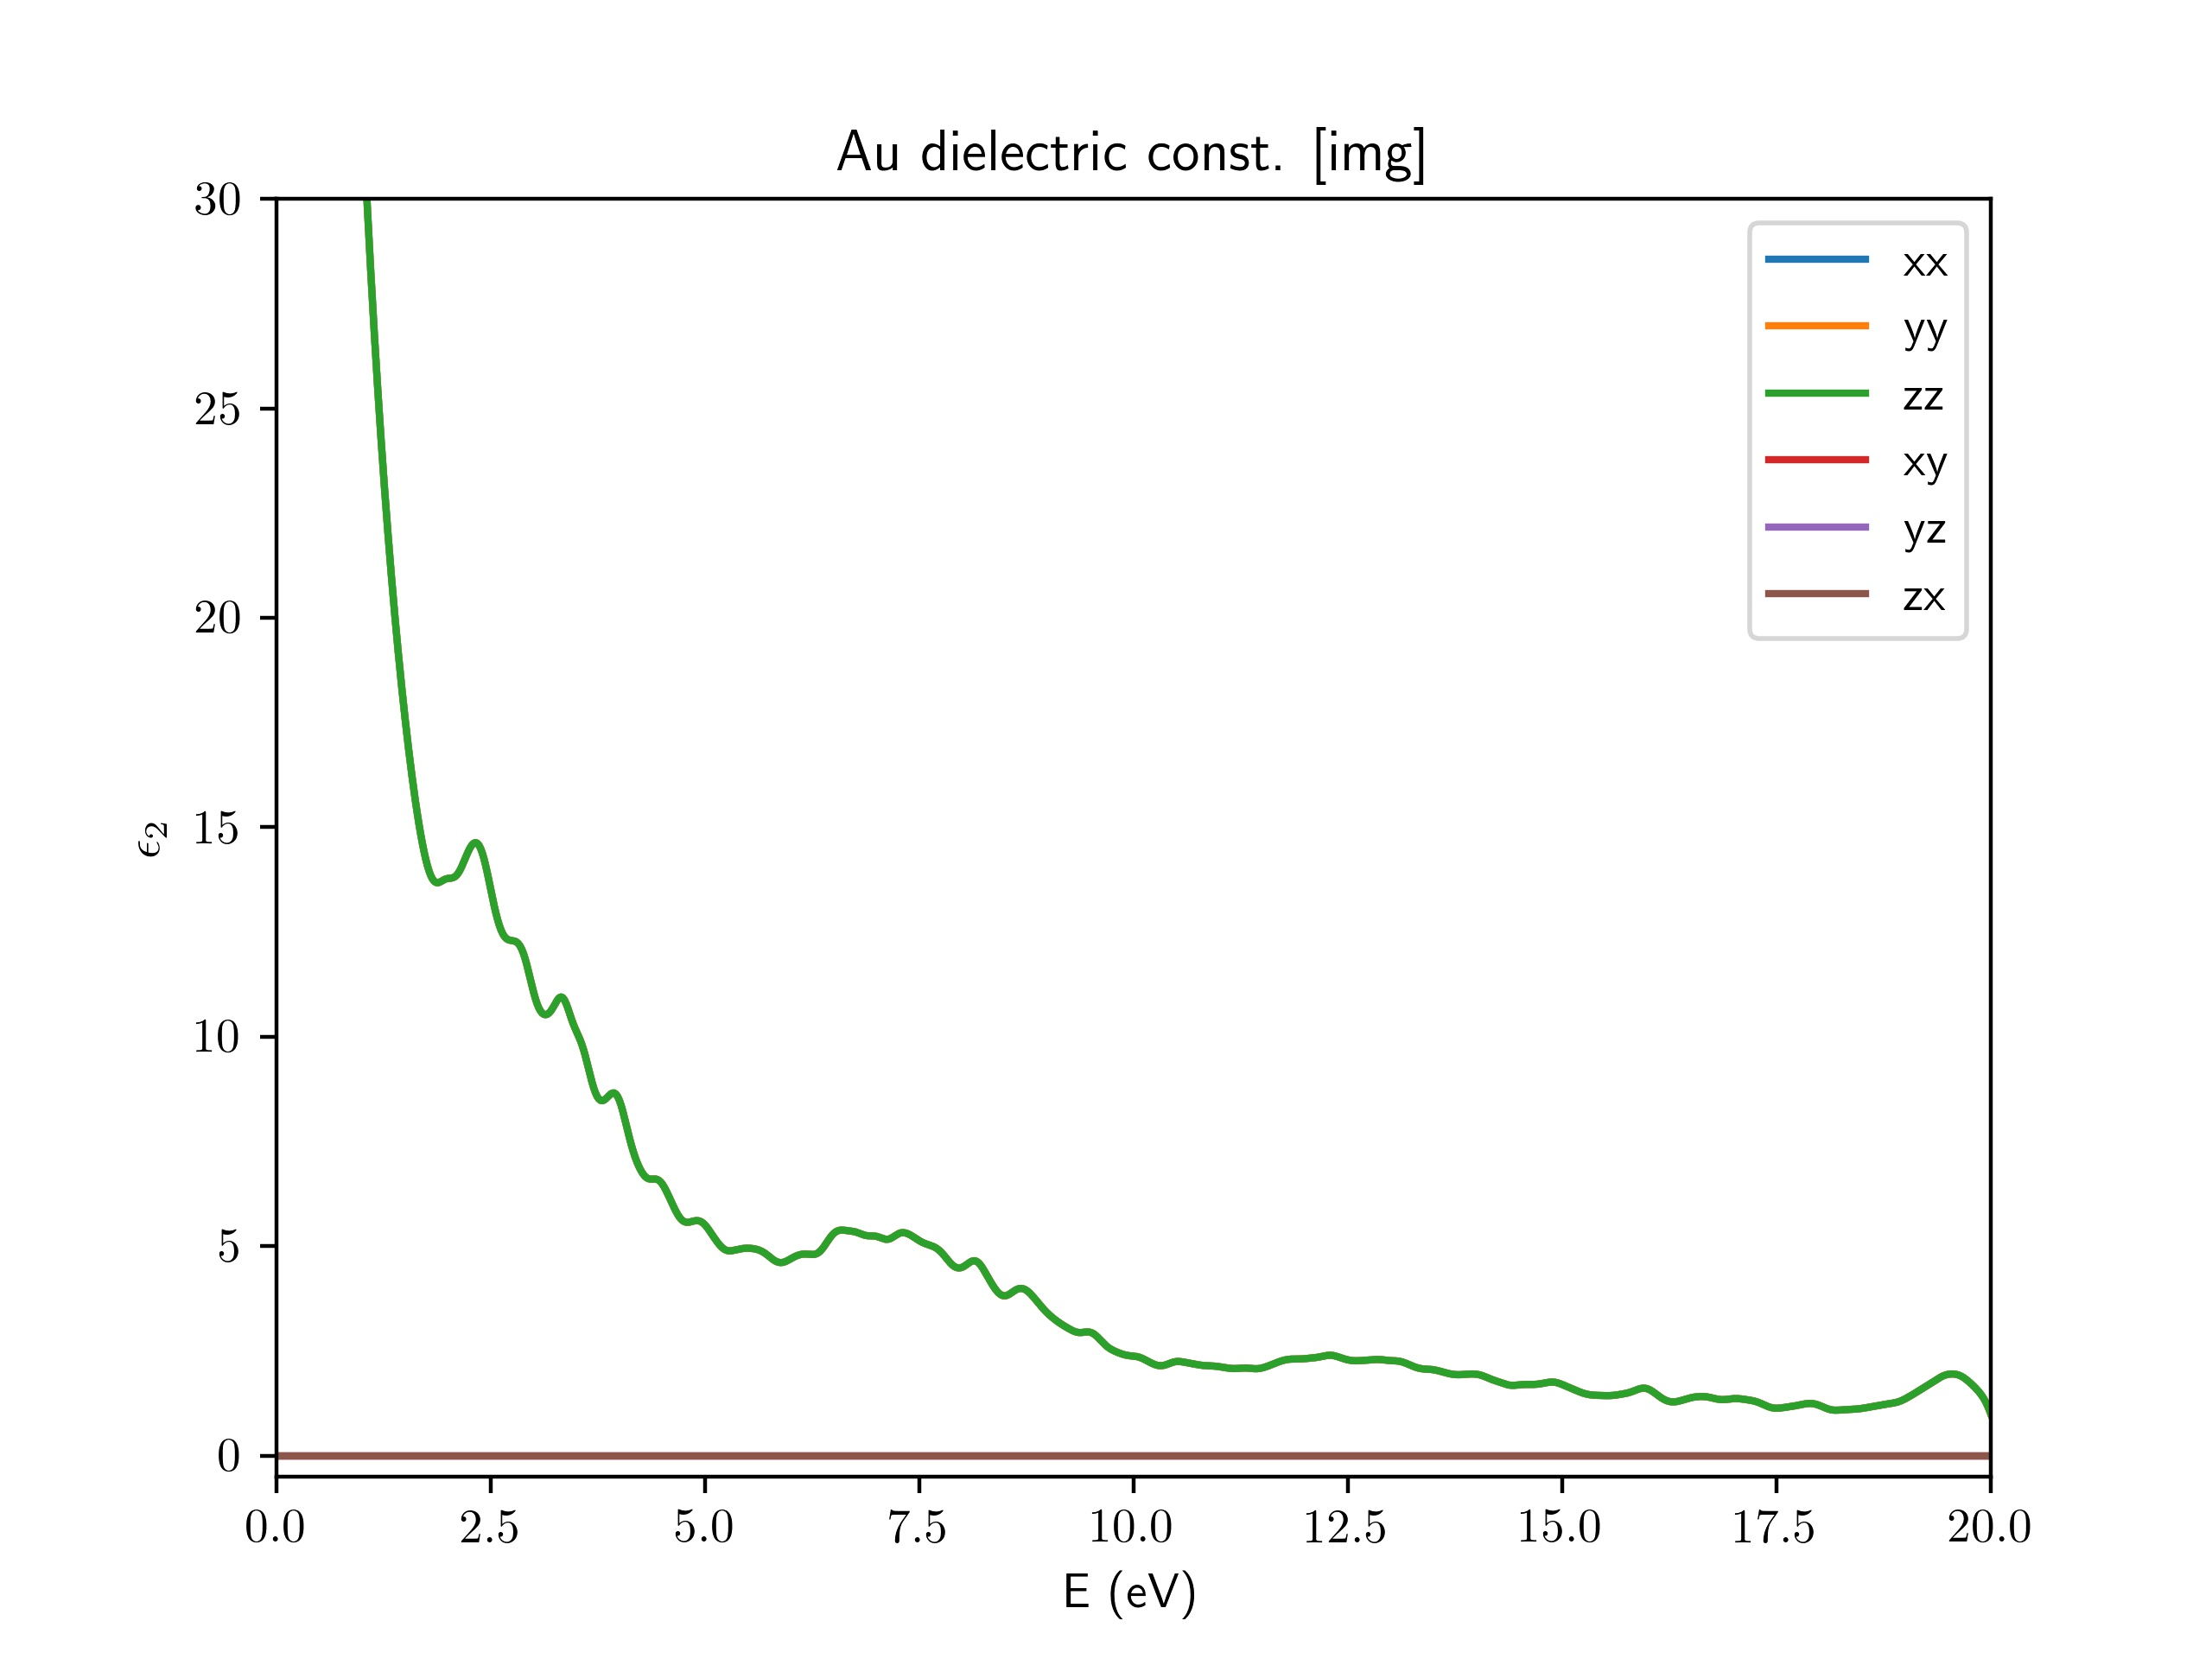
\includegraphics[width=\textwidth]{{data/q2/All_Data/Au_data/Au_epsim}.jpg}
						\caption{Au dielectric constant (image)}
						\label{fig:Auepsim}
					\end{minipage}
					\begin{minipage}[b]{0.45\textwidth}
						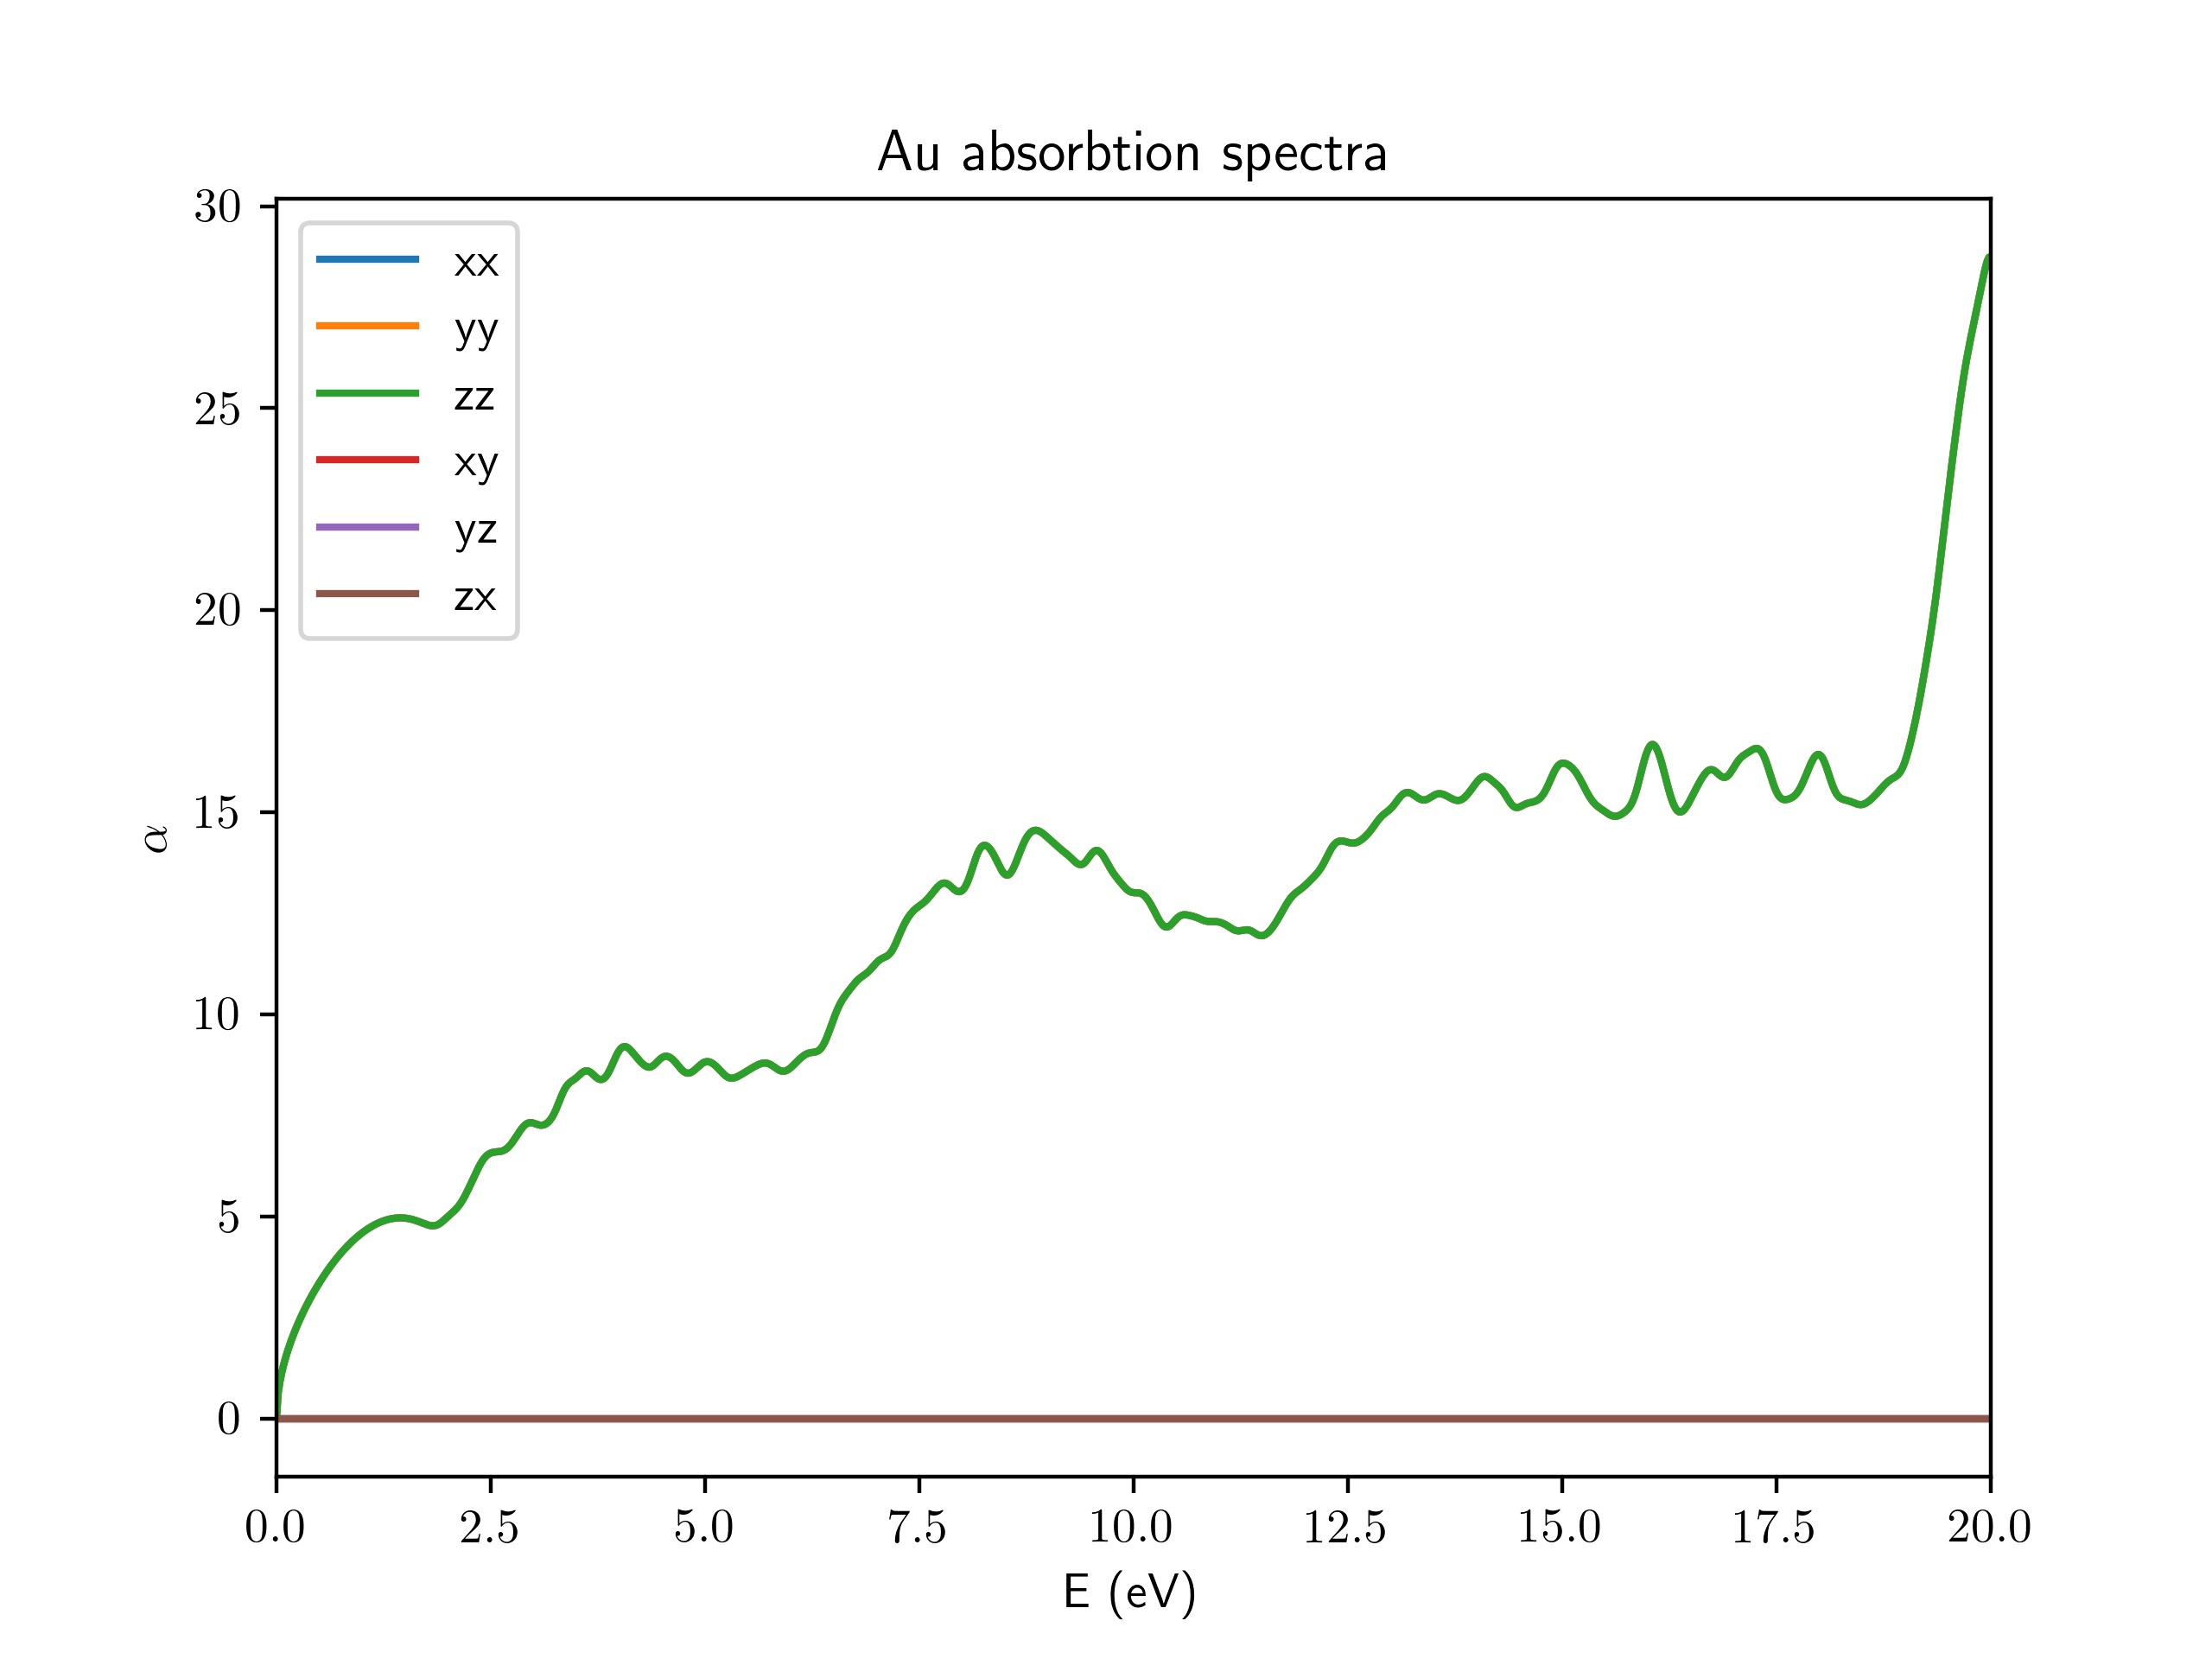
\includegraphics[width=\textwidth]{{data/q2/All_Data/Au_data/Au_alpha}.jpg}
						\caption{Au absorption}
						\label{fig:Aualpha}
					\end{minipage}
				\end{figure} 
				
				
			\clearpage
			\item Si
			
				Following shows the bands structure, density of states for Si without spin orbital coupling(non-relativistic). The calculation are consist with previous study \cite{LIU20151384}
			
				\begin{figure}[h!]
				
					\begin{minipage}[b]{0.45\textwidth}
						\includegraphics[width=\textwidth]{{data/q2/All_Data/Si_data/Si}.jpg}
						\caption{Si band structure}
						\label{fig:Siband}
					\end{minipage}
					\begin{minipage}[b]{0.45\textwidth}
						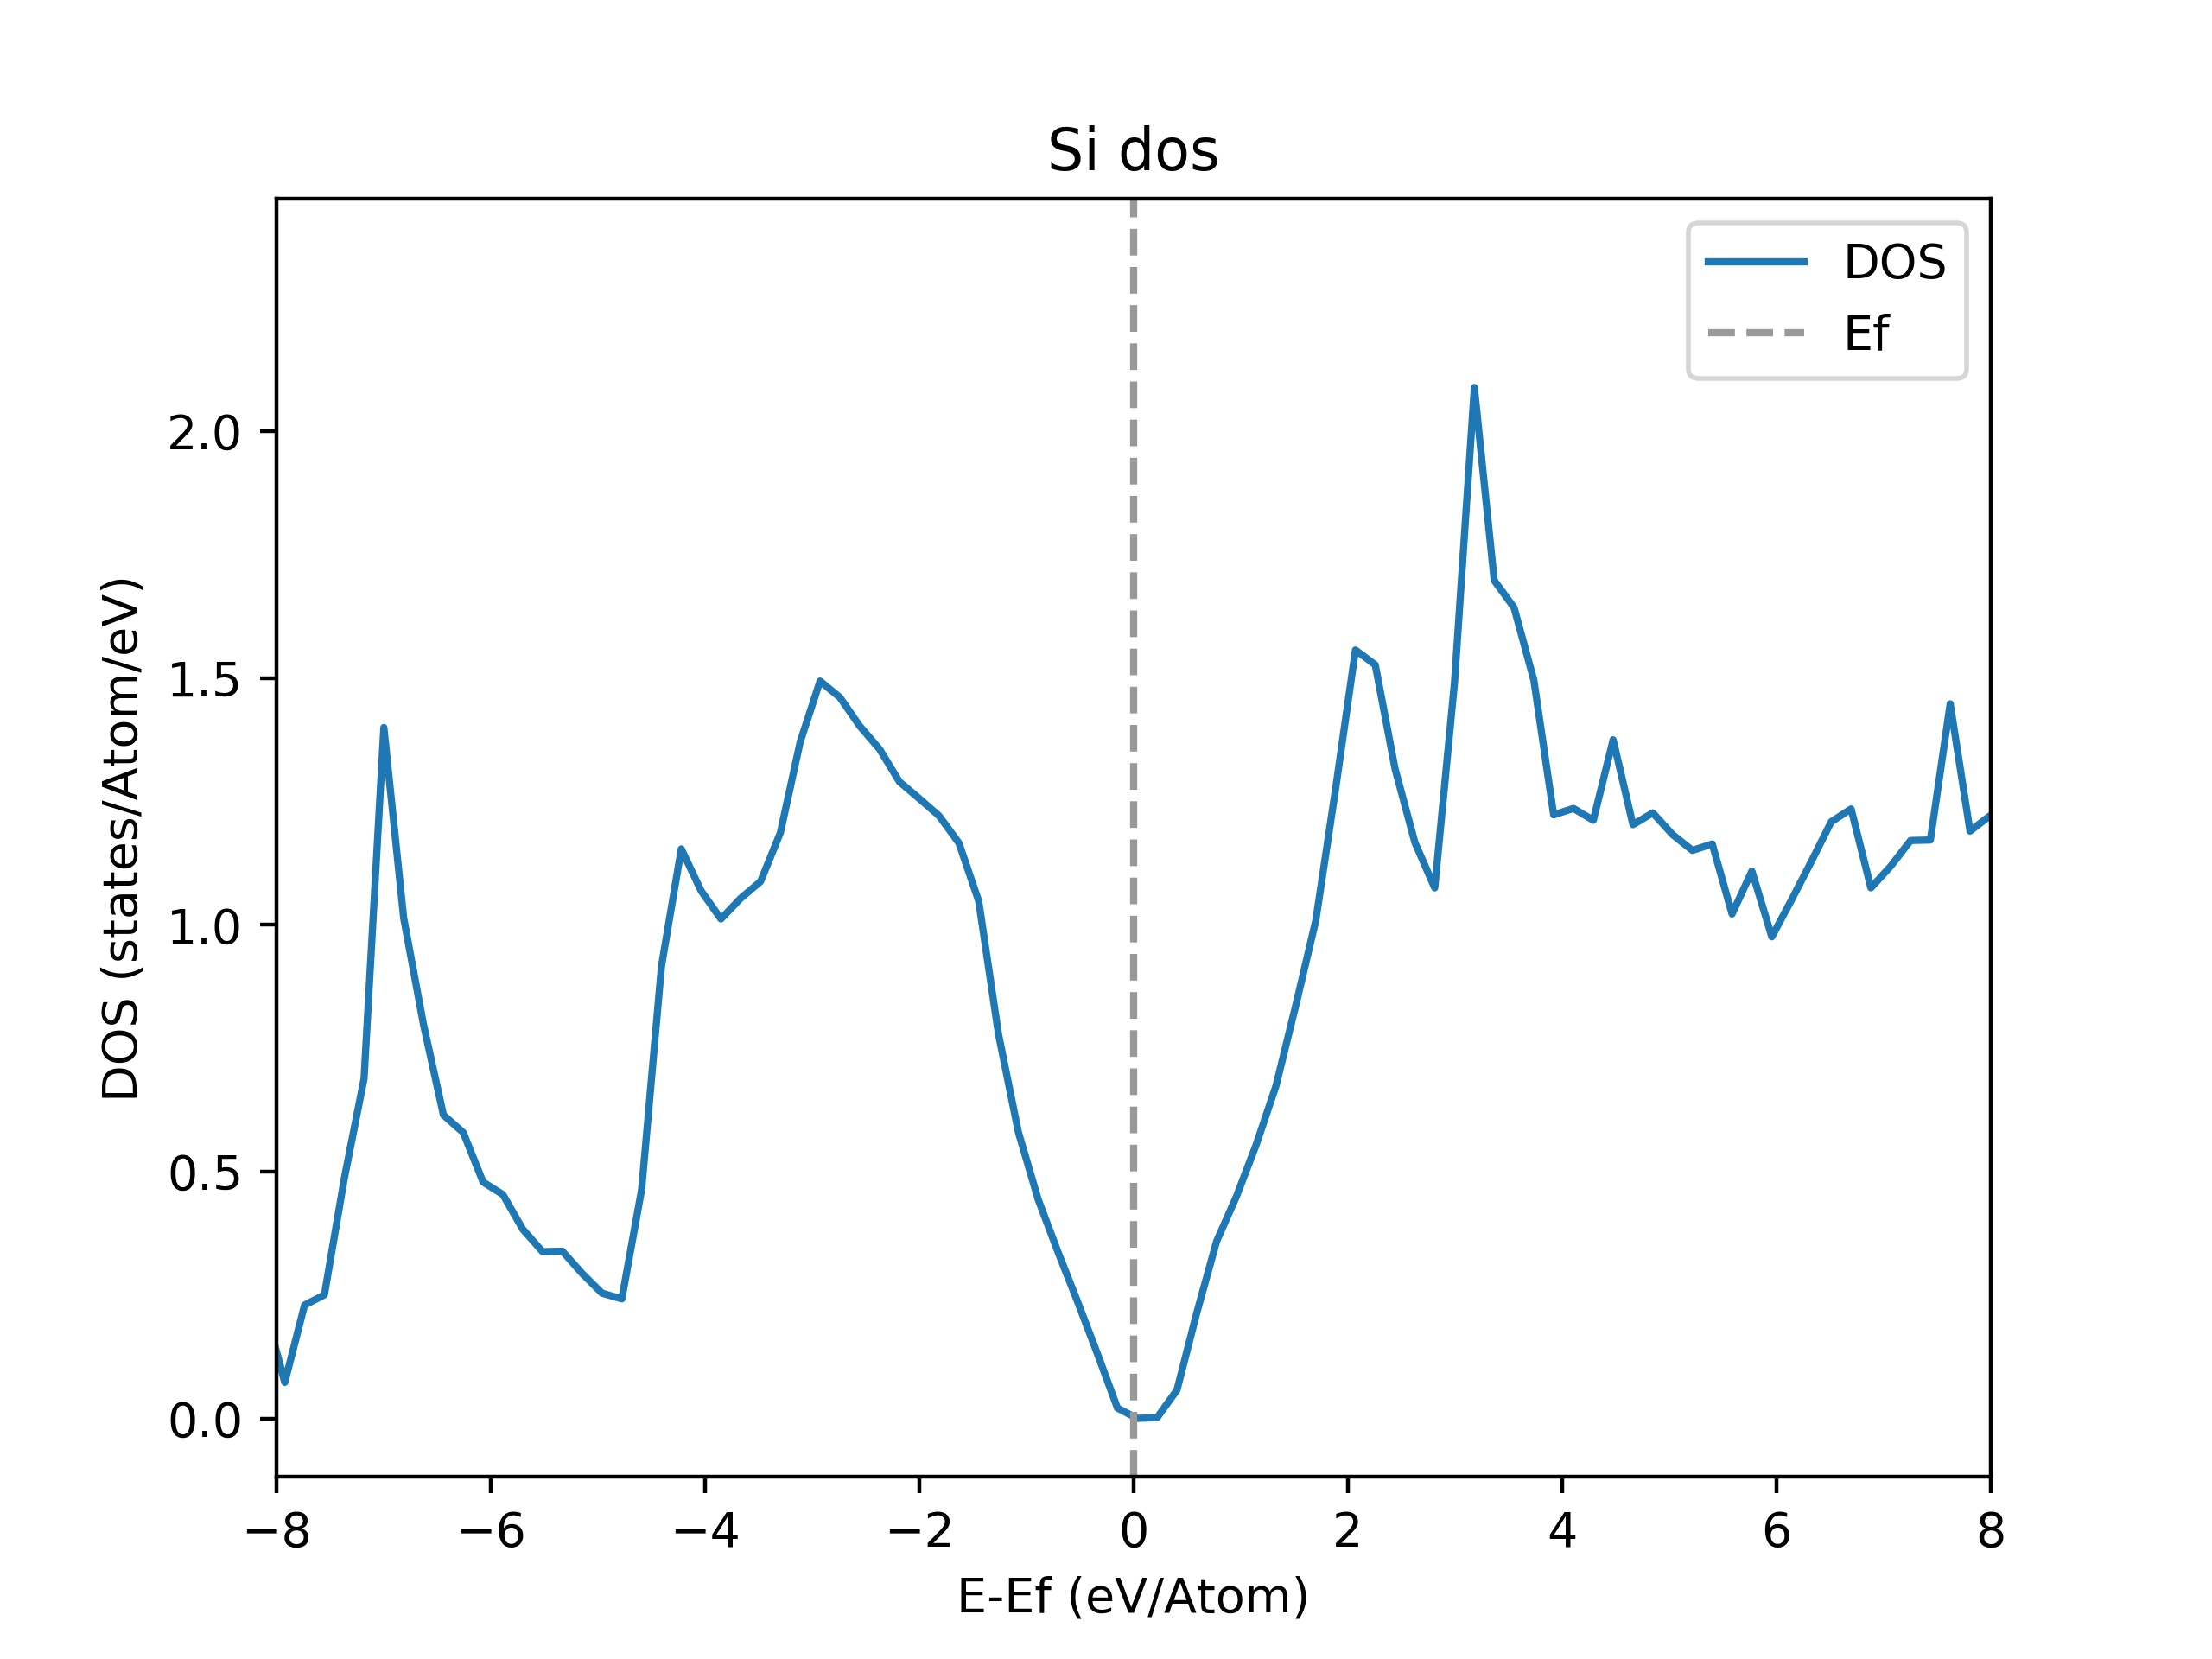
\includegraphics[width=\textwidth]{{data/q2/All_Data/Si_data/Si_dos}.jpg}
						\caption{Si DOS}
						\label{fig:Sidos}
					\end{minipage}
					\begin{minipage}[b]{0.45\textwidth}
						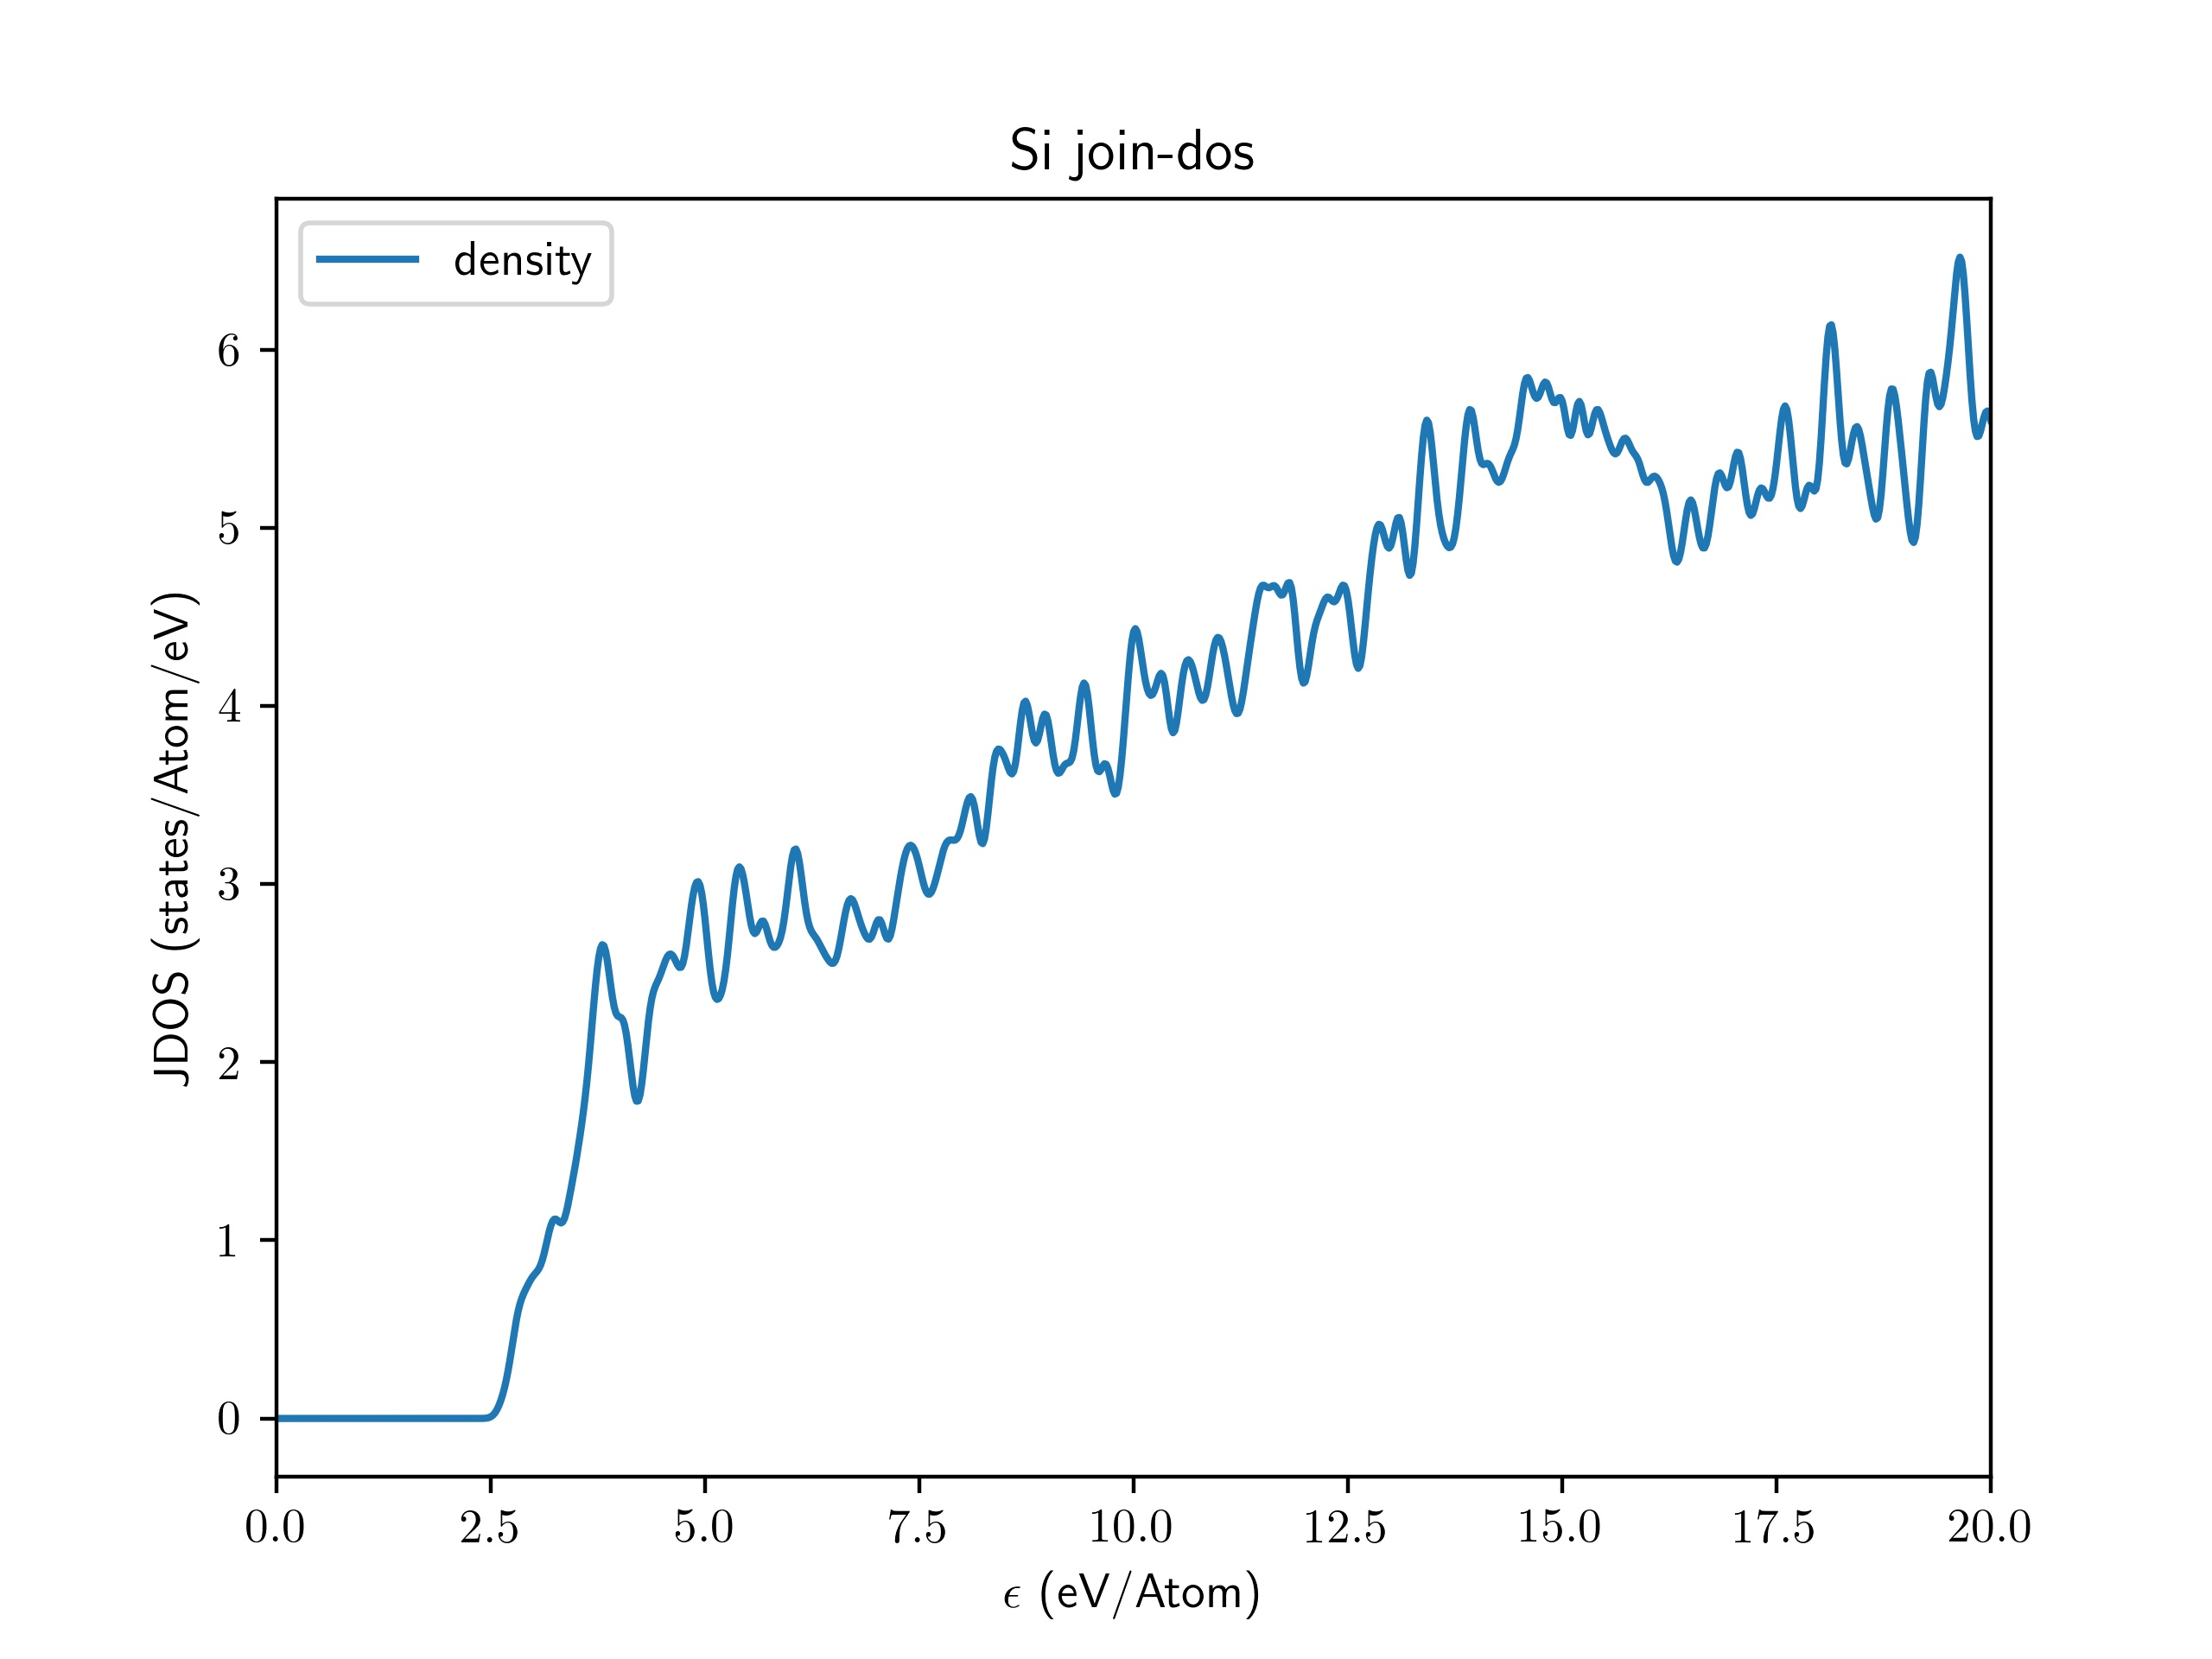
\includegraphics[width=\textwidth]{{data/q2/All_Data/Si_data/Si_jdos}.jpg}
						\caption{Si join-DOS}
						\label{fig:Sijdos}
					\end{minipage}
					\begin{minipage}[b]{0.45\textwidth}
						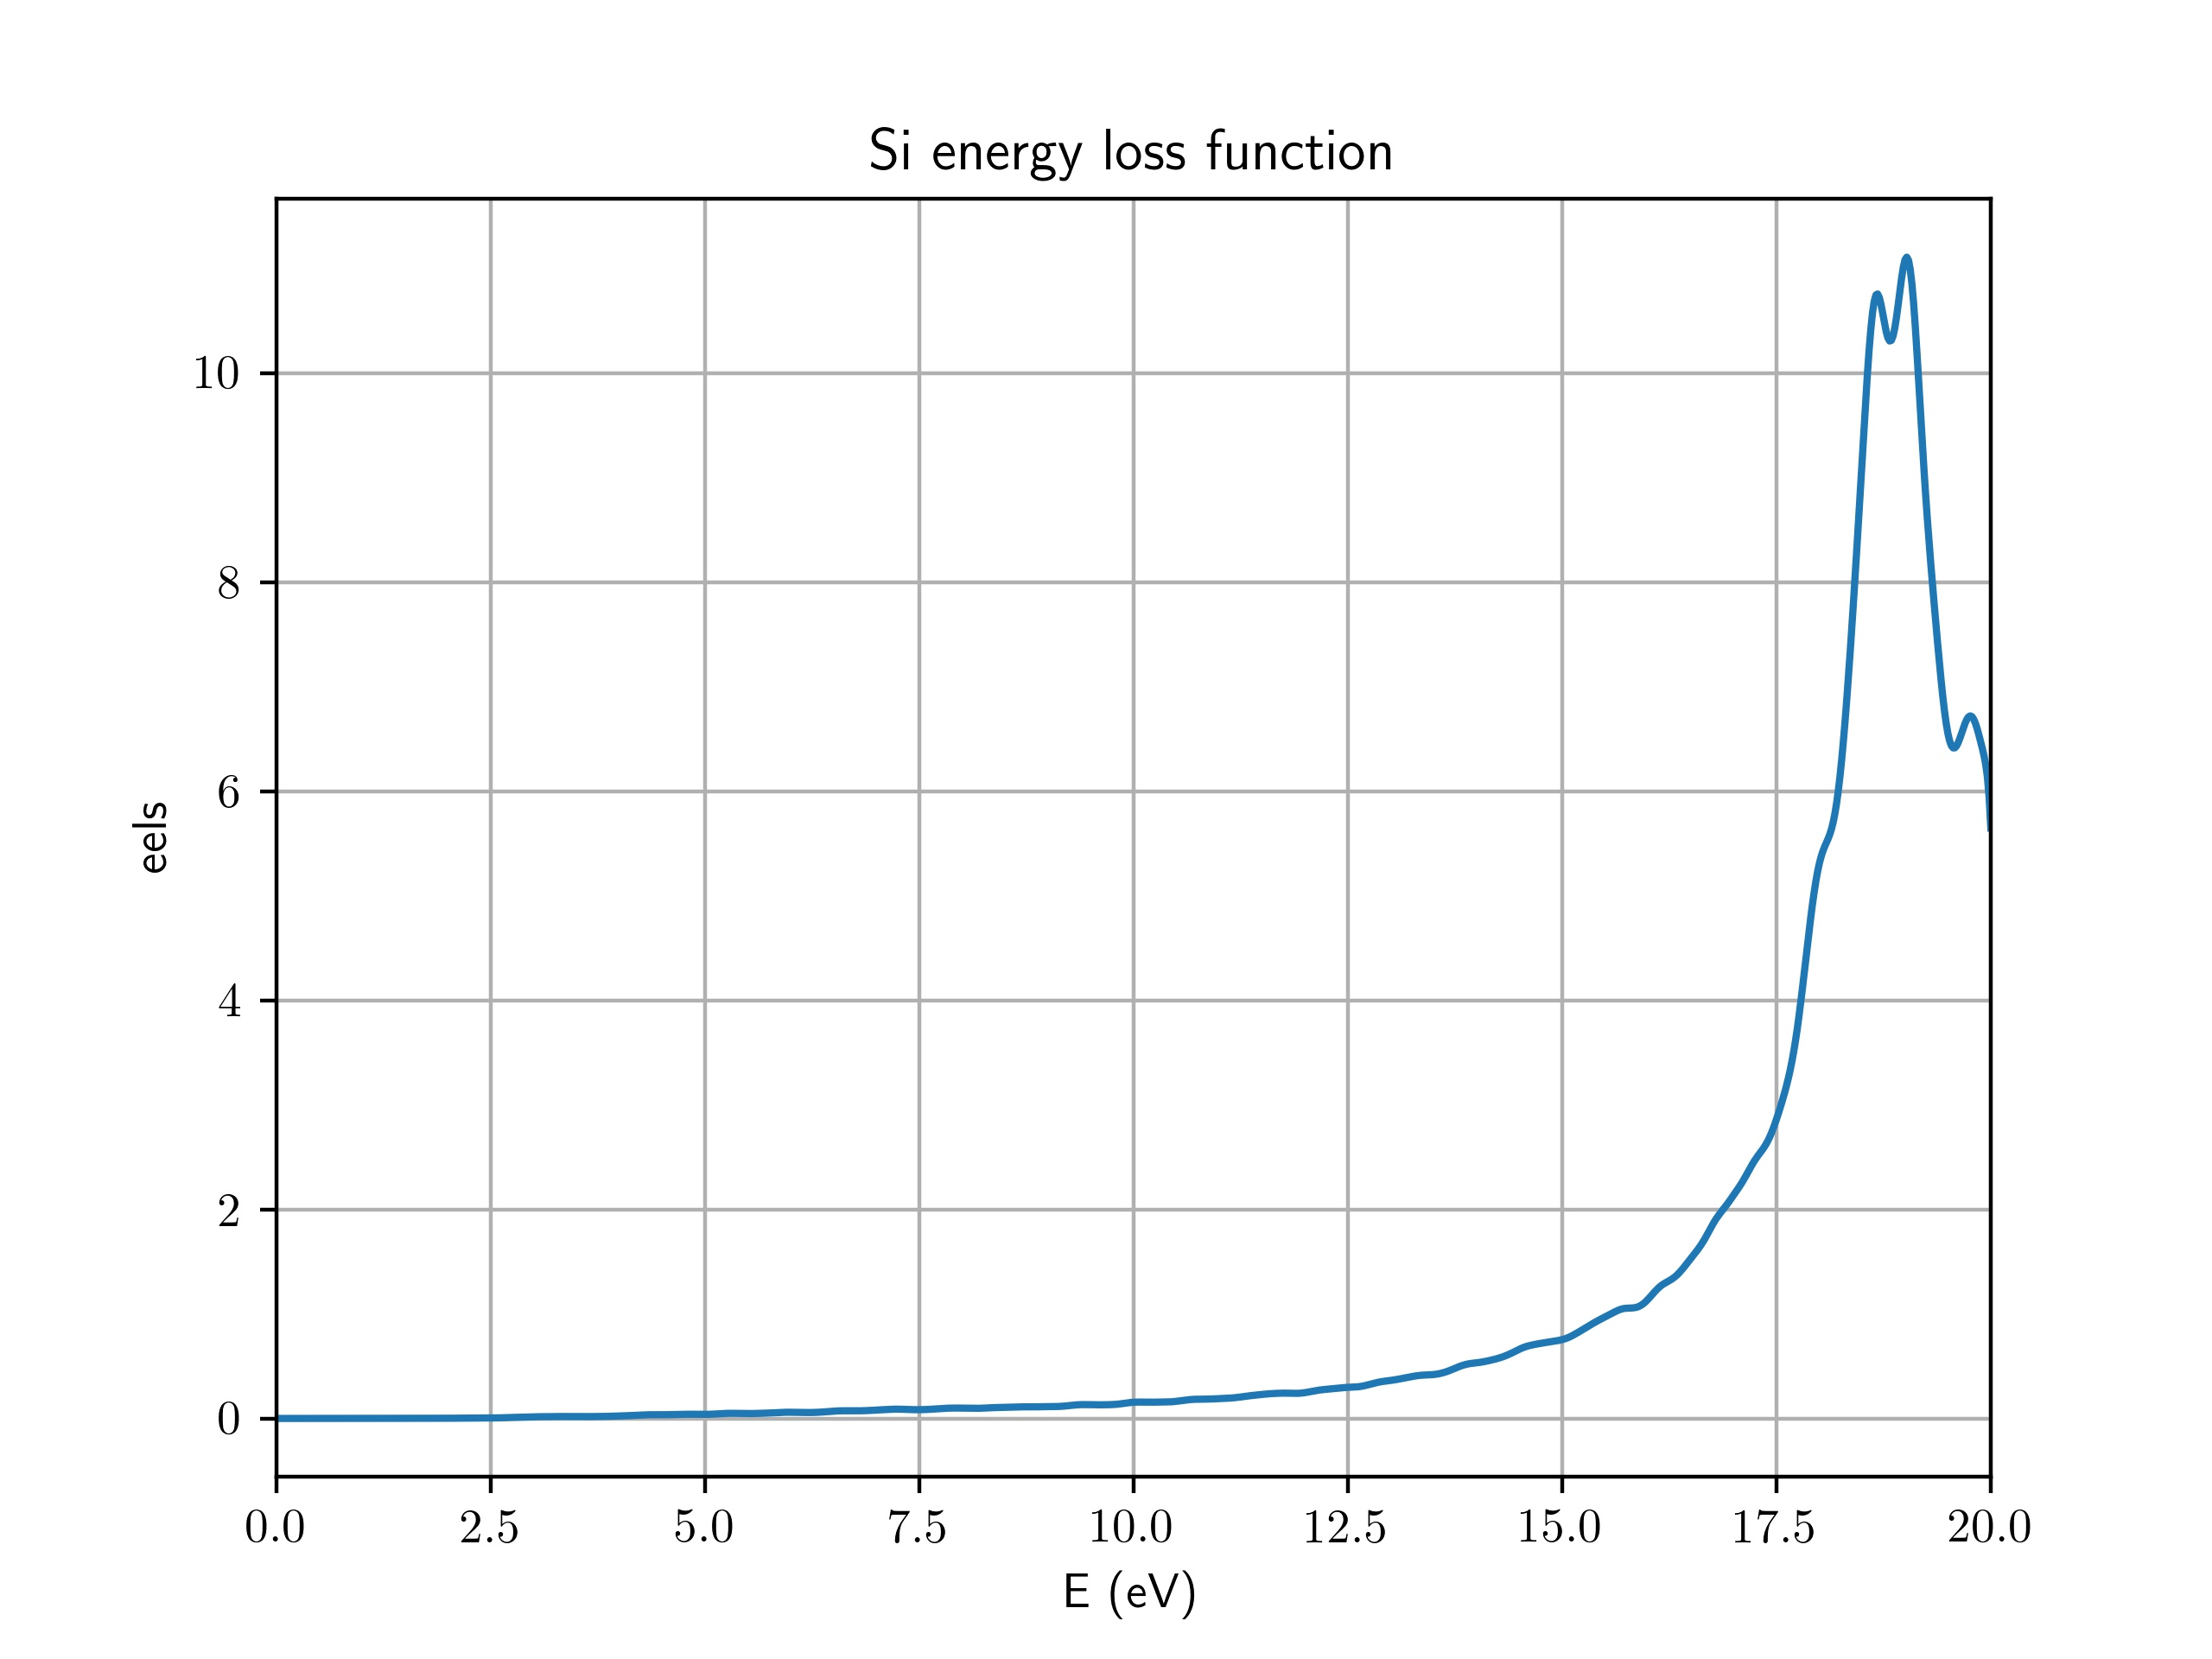
\includegraphics[width=\textwidth]{{data/q2/All_Data/Si_data/Si_eels}.jpg}
						\caption{Si energy loss function}
						\label{fig:Sieels}
					\end{minipage}
				\end{figure}
				\begin{figure}[h!]
					\begin{minipage}[b]{0.45\textwidth}
						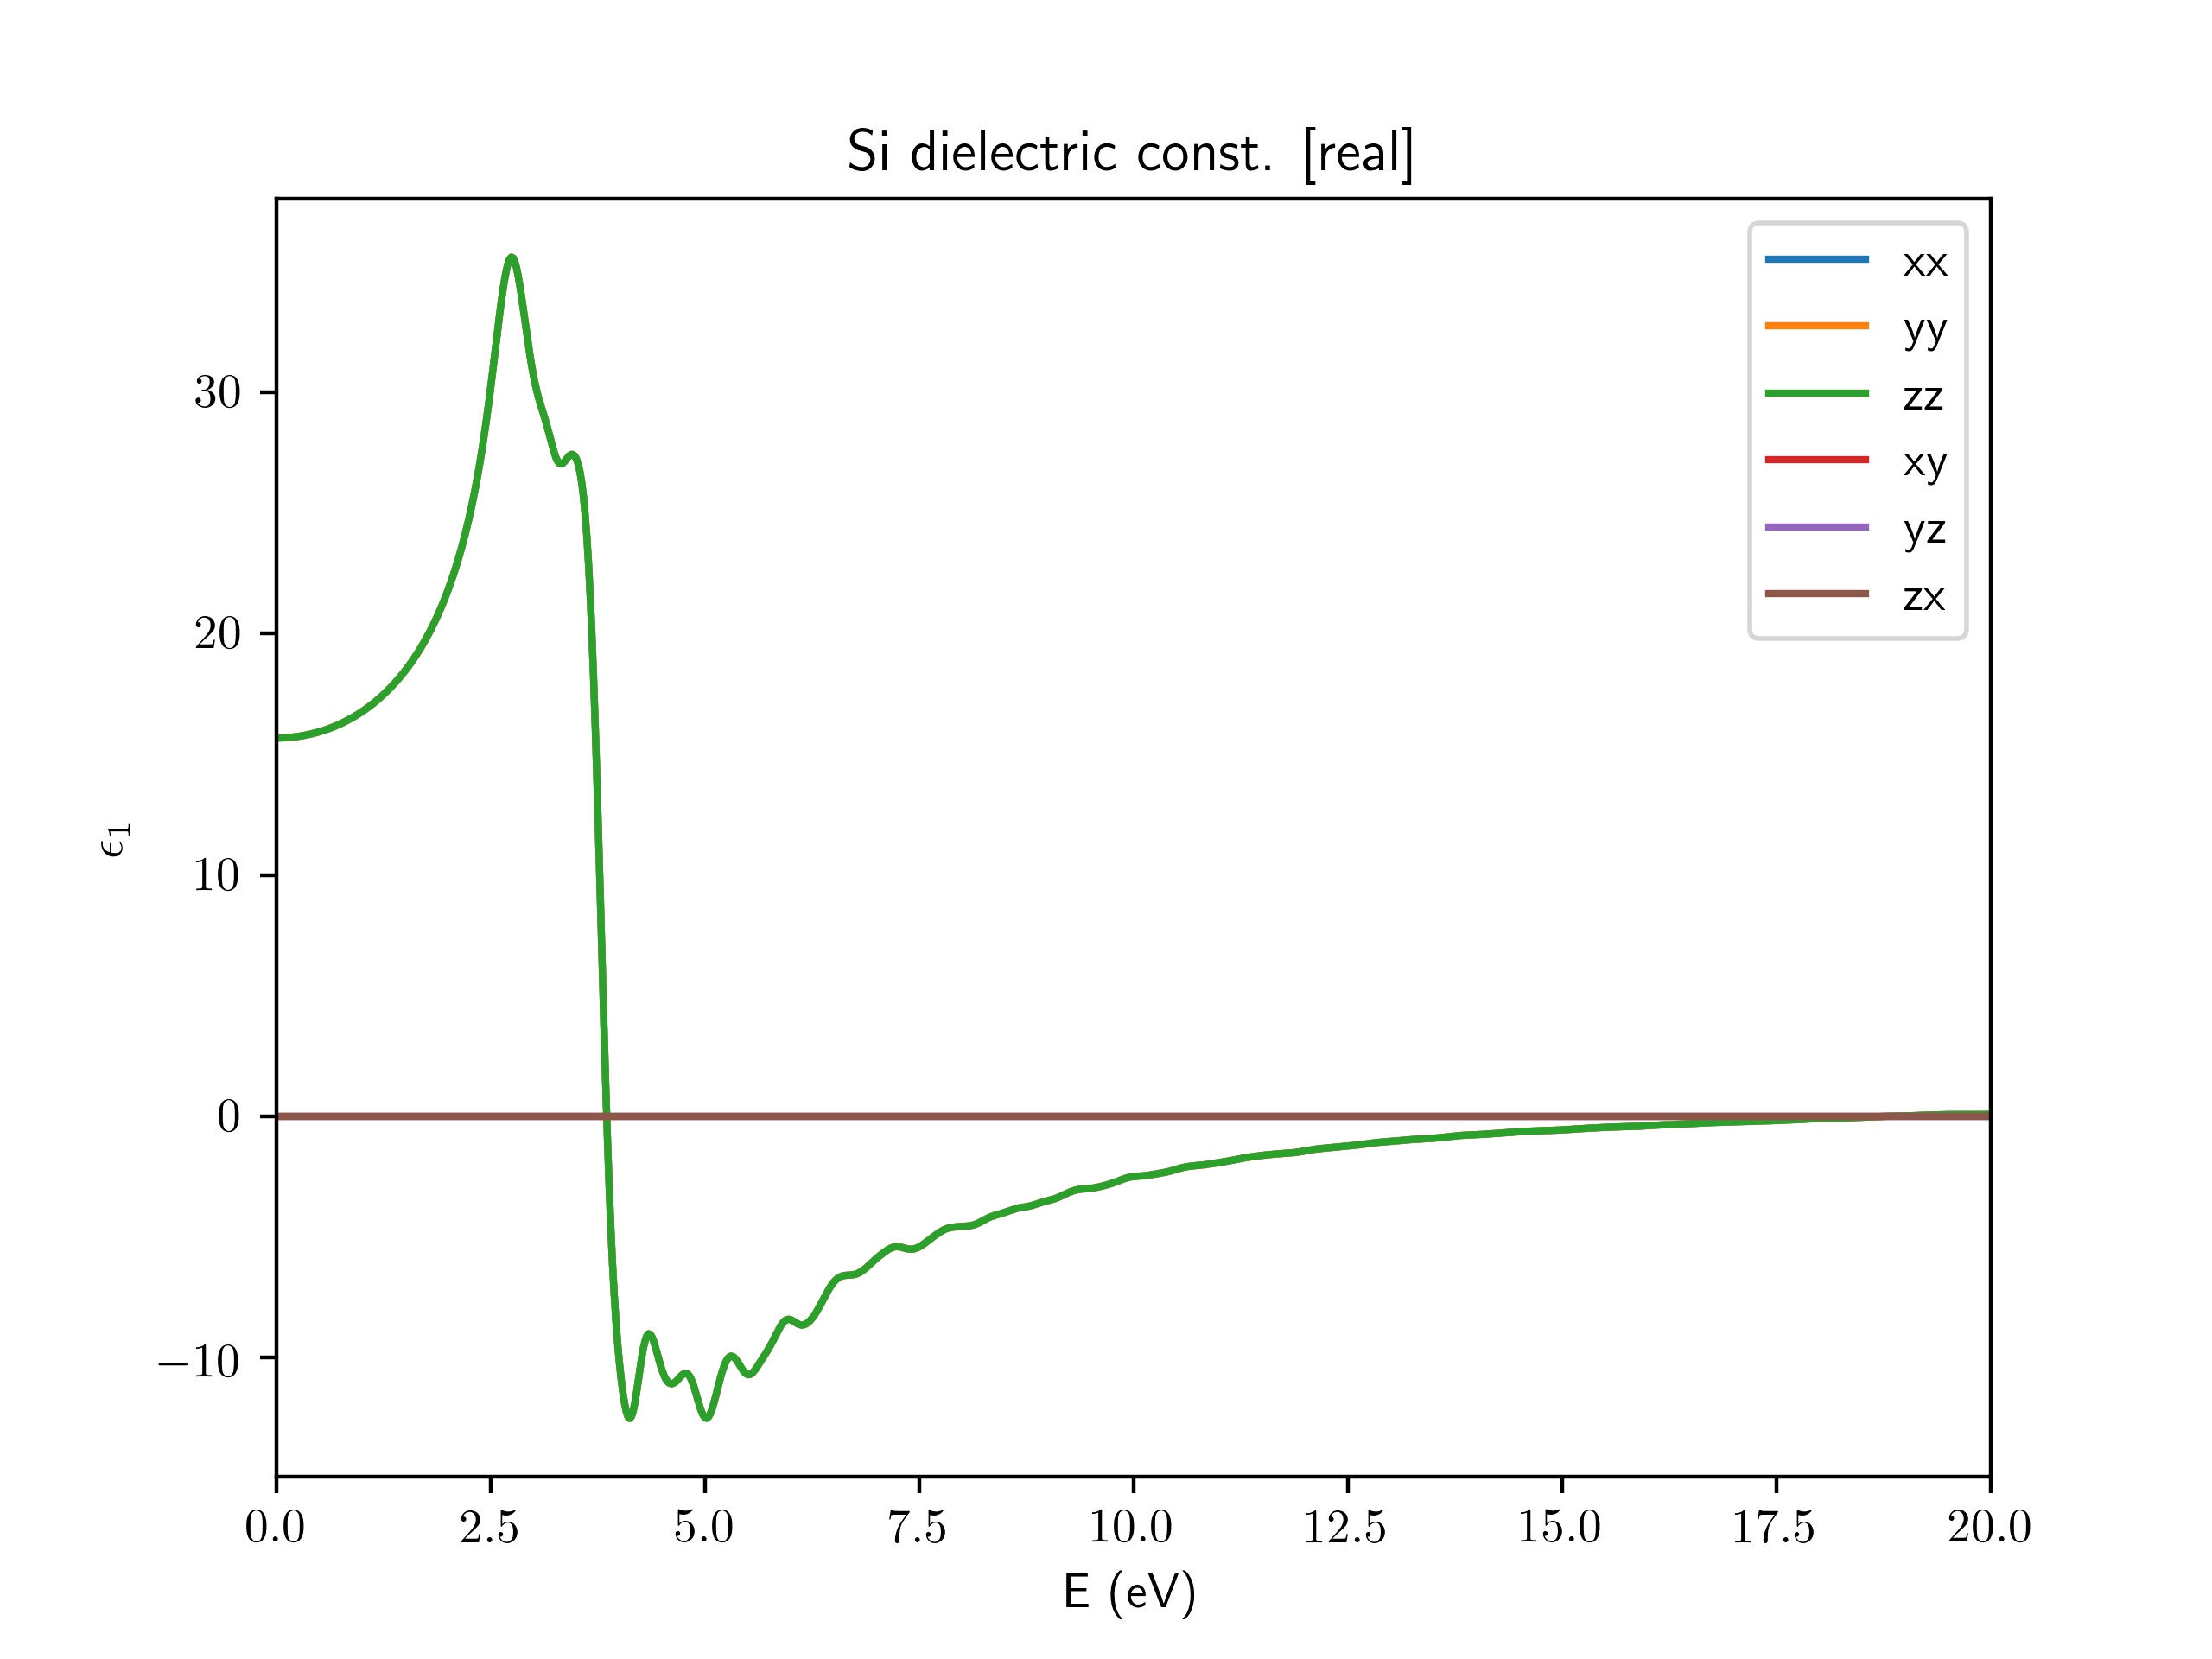
\includegraphics[width=\textwidth]{{data/q2/All_Data/Si_data/Si_epsre}.jpg}
						\caption{Si dielectric constant (real)}
						\label{fig:Siepsre}
					\end{minipage}
					\begin{minipage}[b]{0.45\textwidth}
						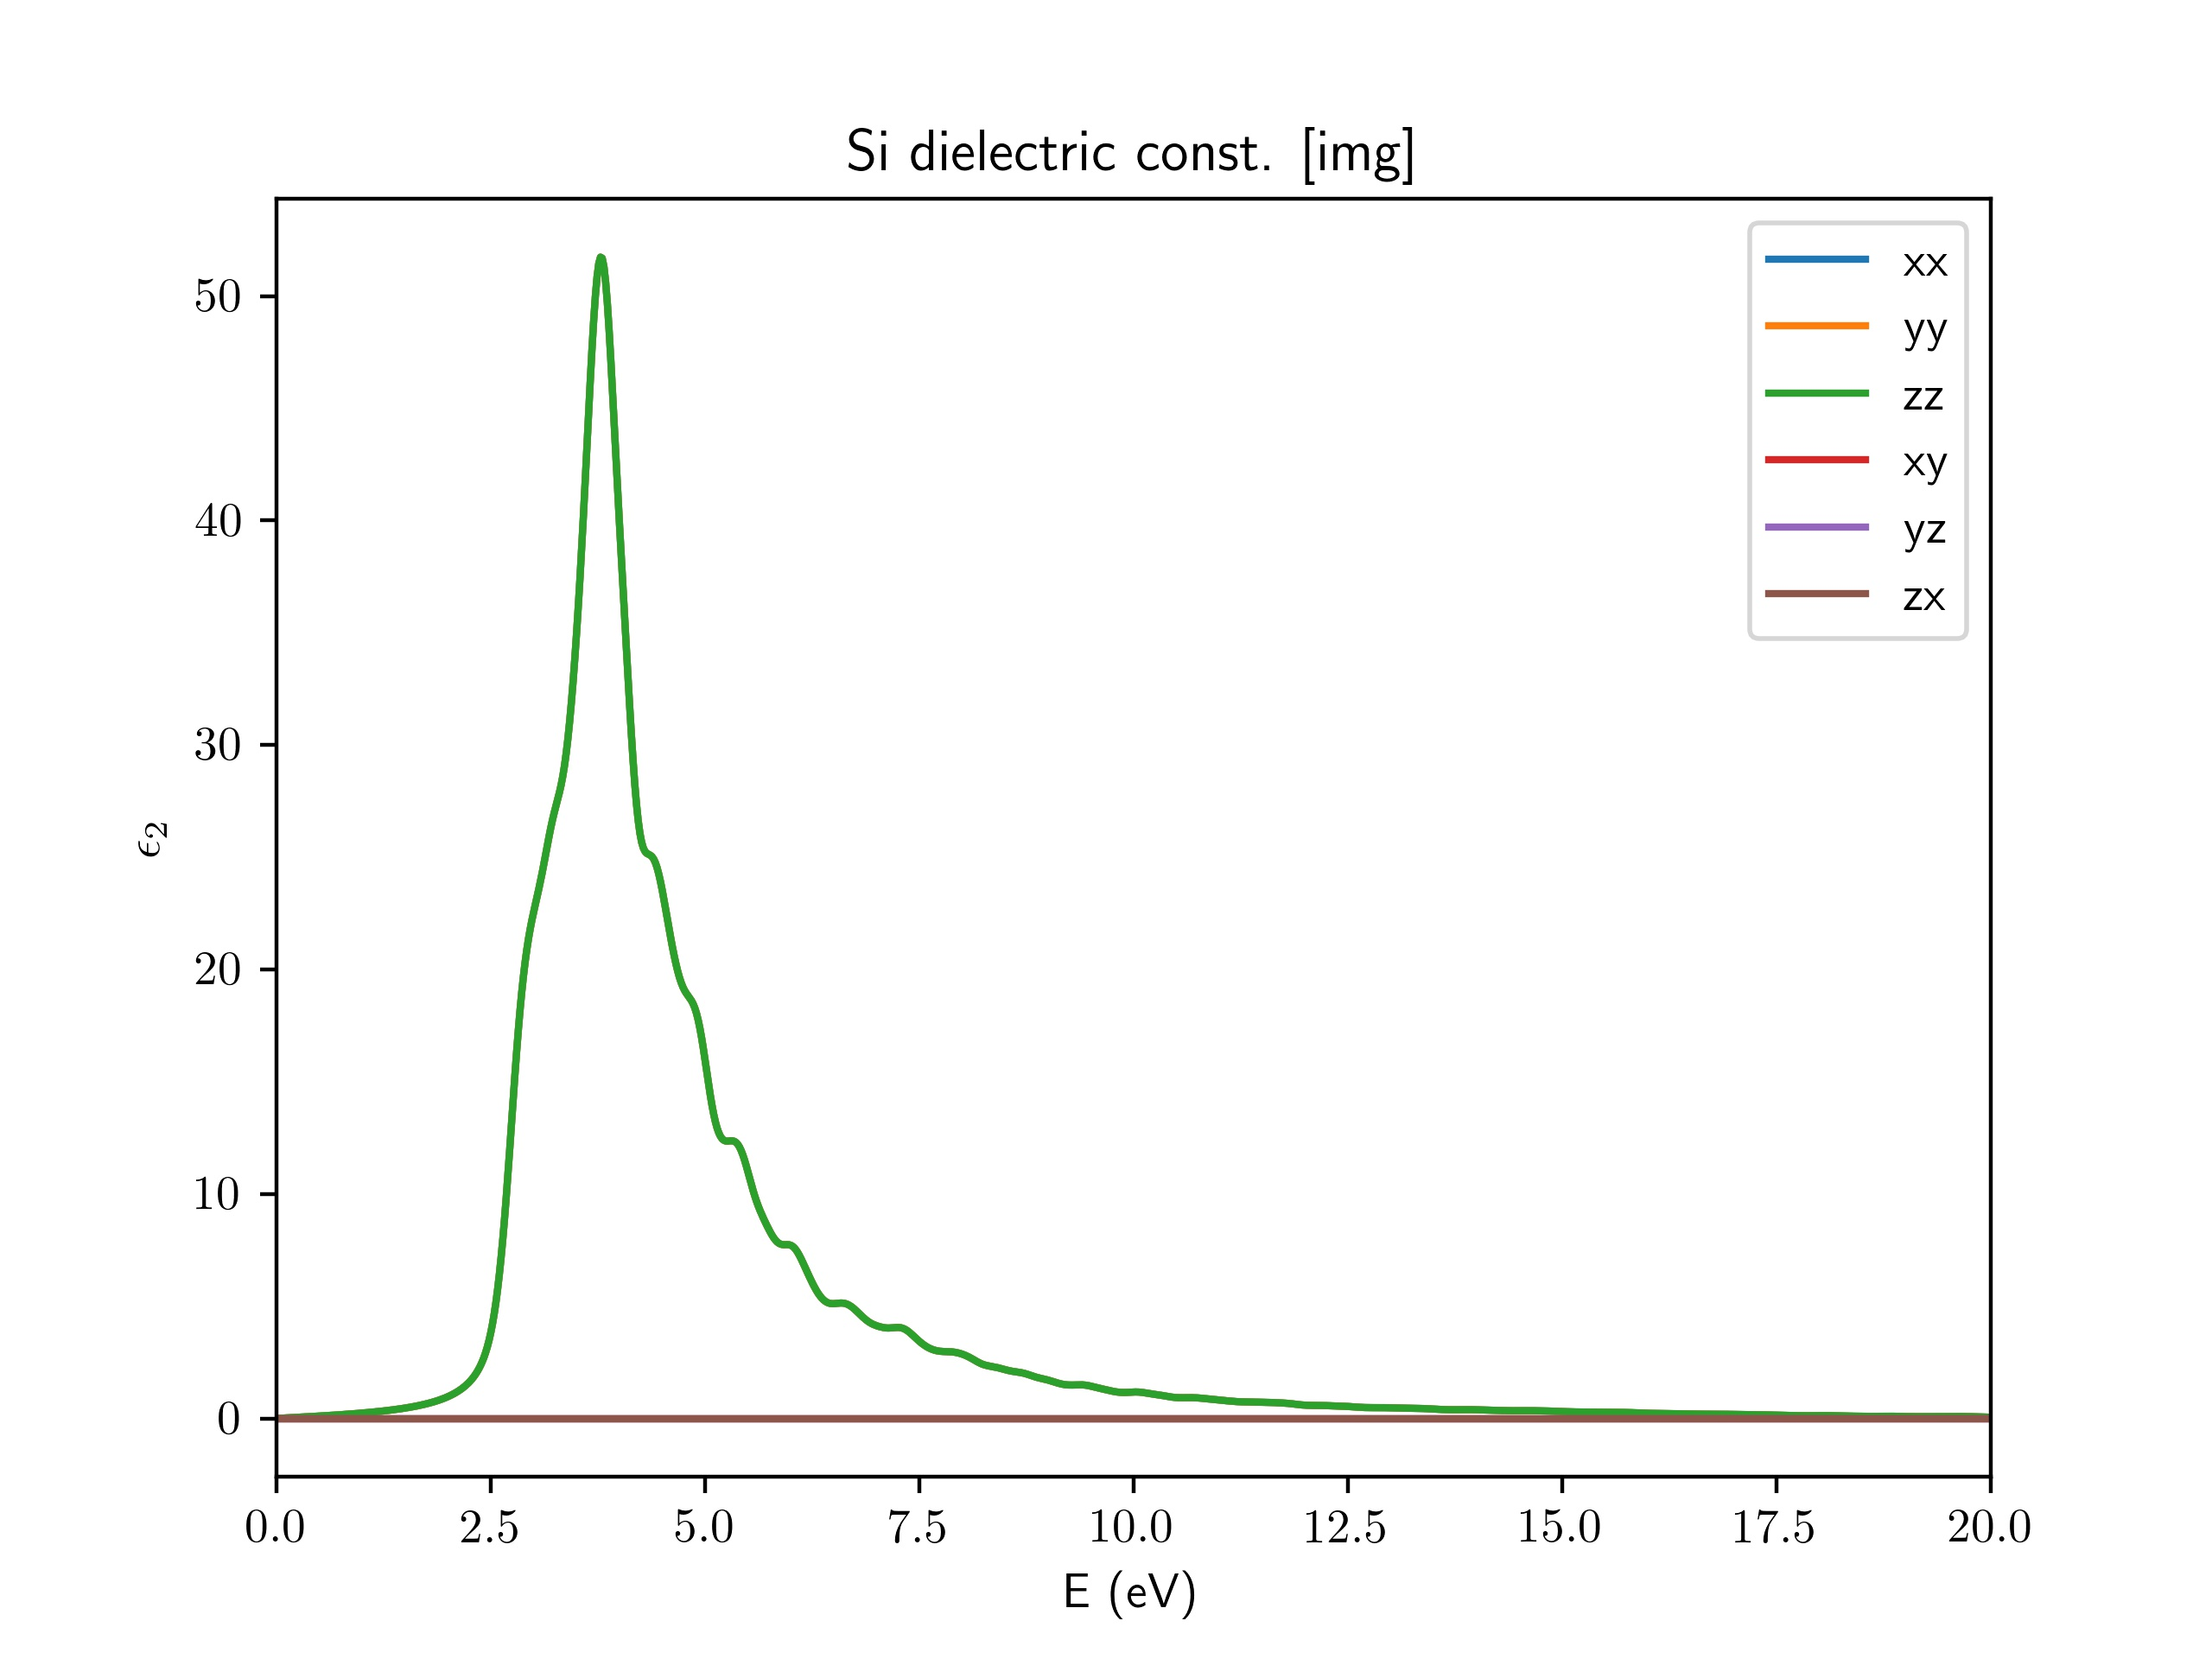
\includegraphics[width=\textwidth]{{data/q2/All_Data/Si_data/Si_epsim}.jpg}
						\caption{Si dielectric constant (image)}
						\label{fig:Siepsim}
					\end{minipage}
					\begin{minipage}[b]{0.45\textwidth}
						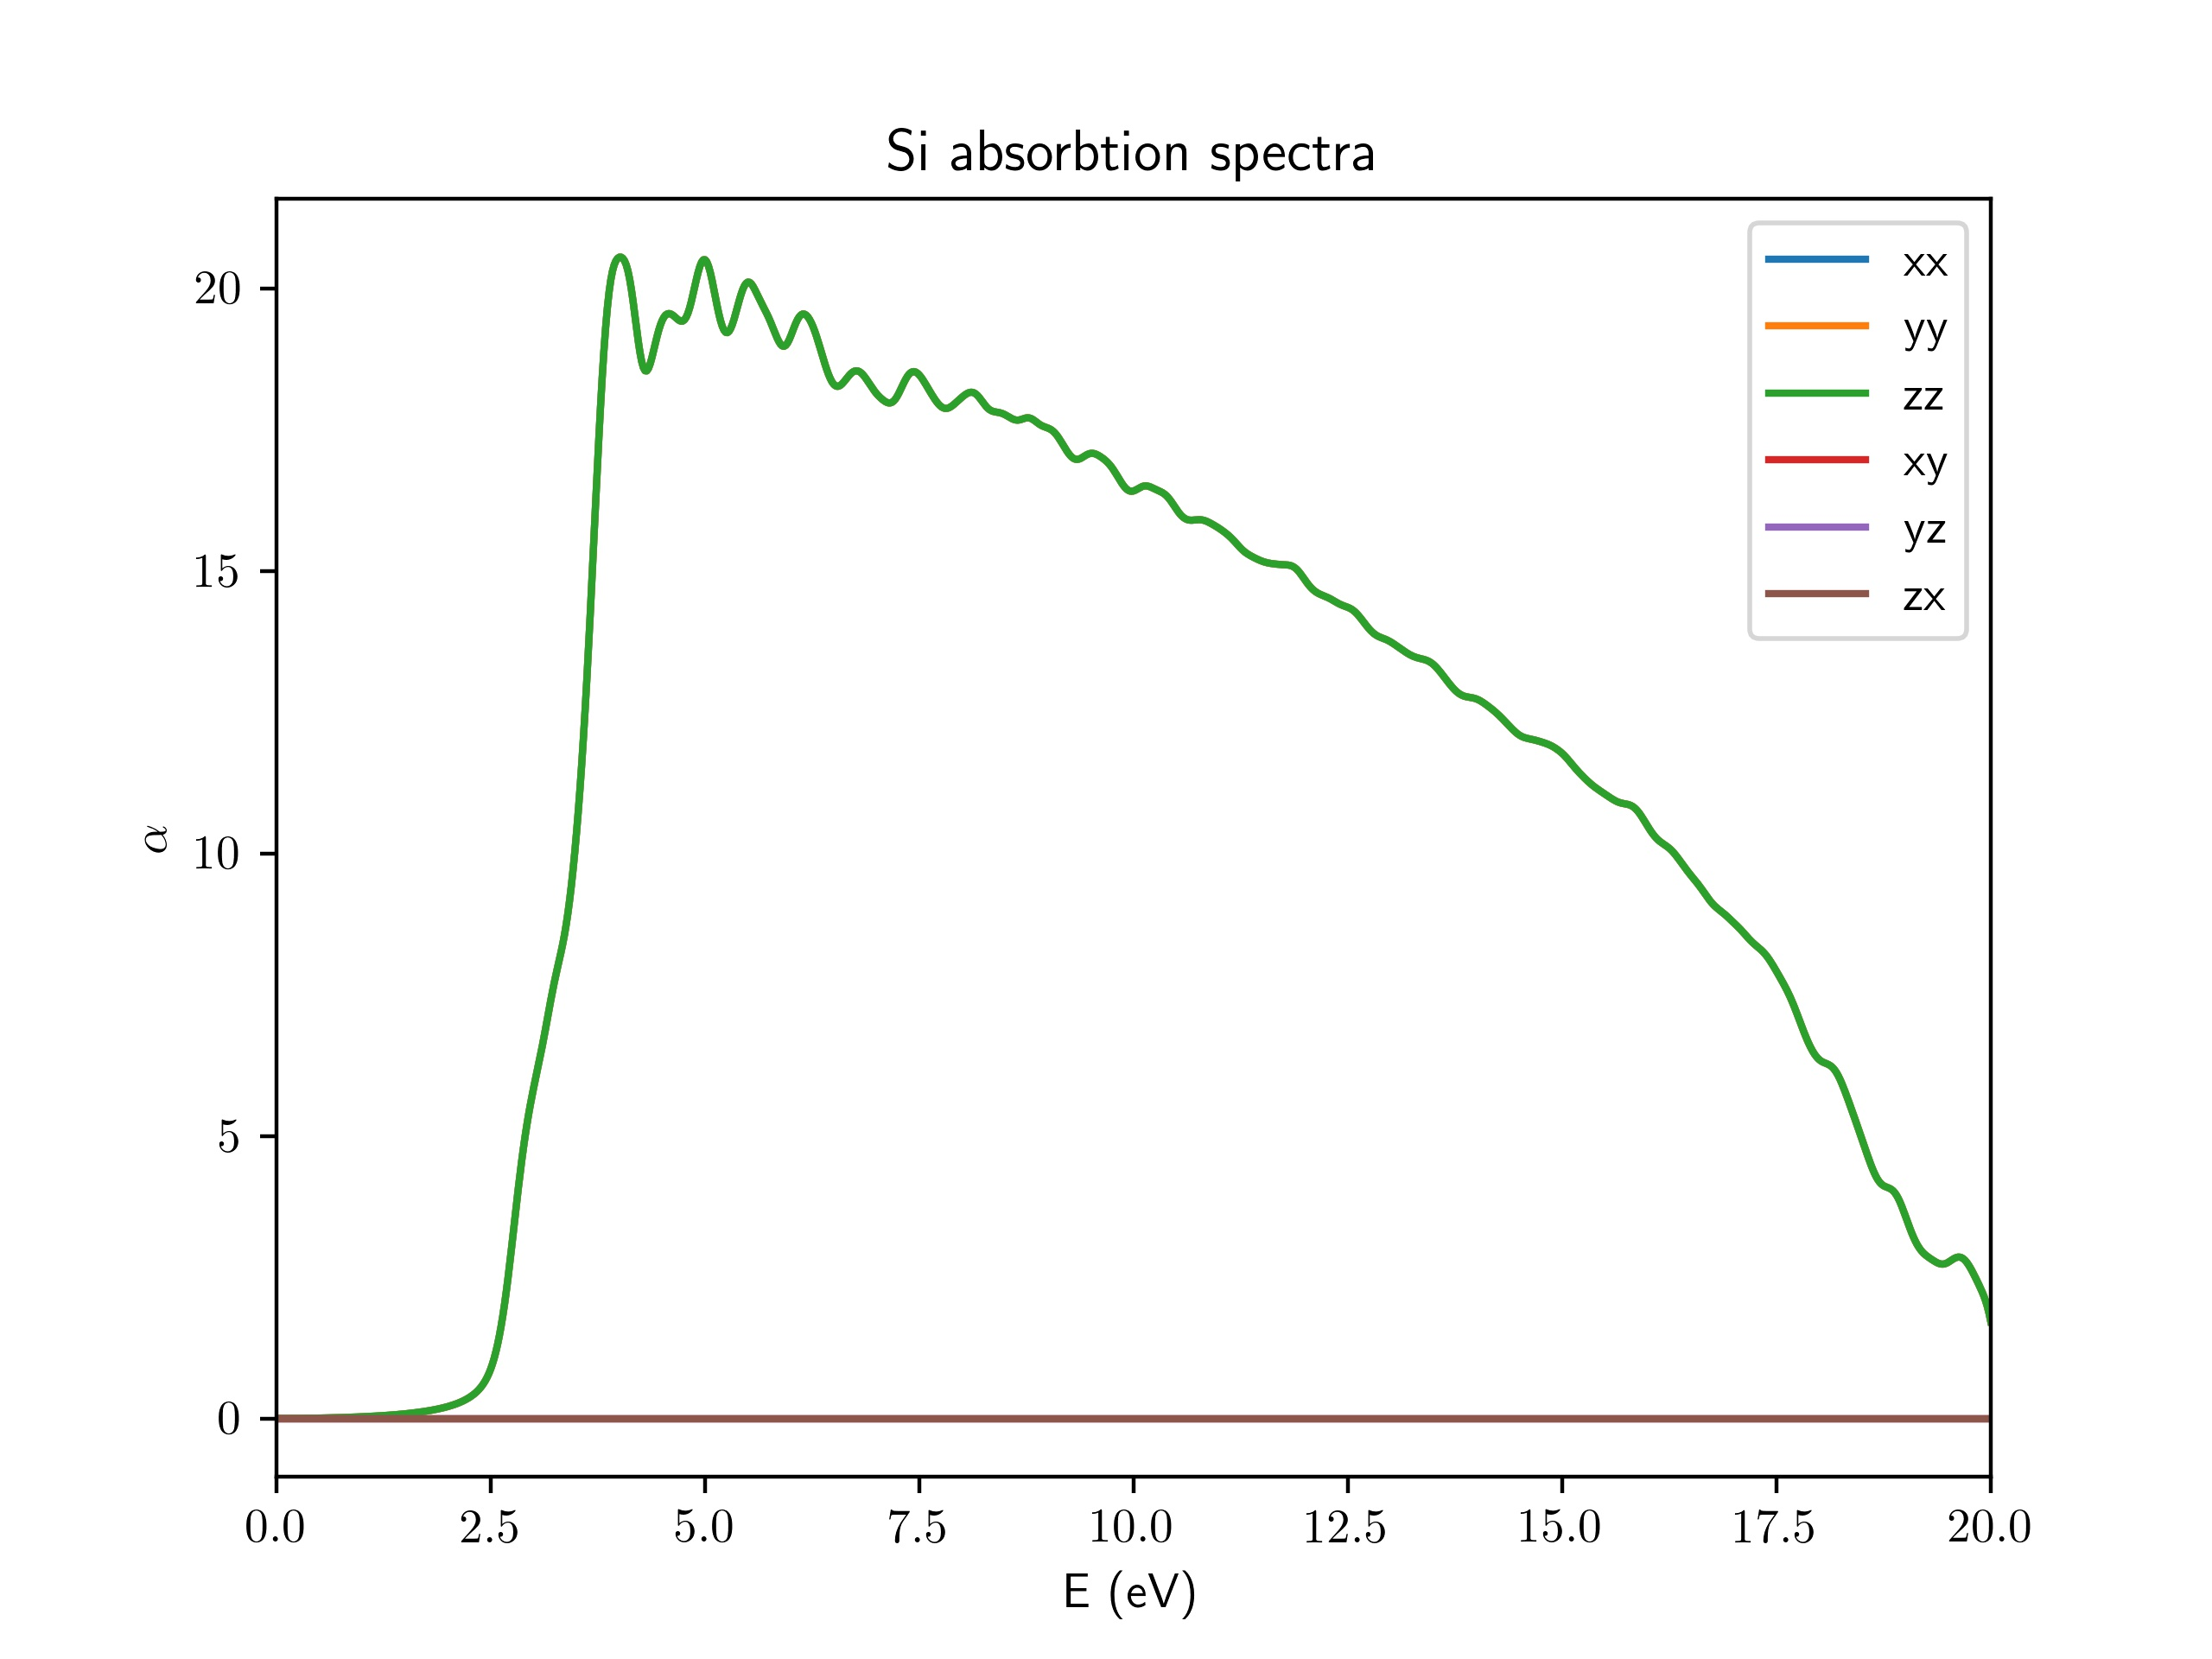
\includegraphics[width=\textwidth]{{data/q2/All_Data/Si_data/Si_alpha}.jpg}
						\caption{Si absorption}
						\label{fig:Sialpha}
					\end{minipage}
				\end{figure} 
			
		\end{itemize}
	
	
		\clearpage
		\item The calculation results of fcc-Au and diamond-Si with spin-orbital coupling. 
		
		\begin{itemize}
			\item Au
			
			Following shows the bands structure, density of state for Au with spin orbital coupling (relativistic). The calculation of band structure and dos are consist with previous study \cite{JoPAu} \cite{0022-3719-3-2S-301} . Compare with the non-relativistic calculation, we see that the band splitting that due to the spin-orbital coupling can be observe in band structure. Also, The density of states are re-configured when consider the SOC effect. 
			
			\begin{figure}[h!]
				
				\begin{minipage}[b]{0.45\textwidth}
					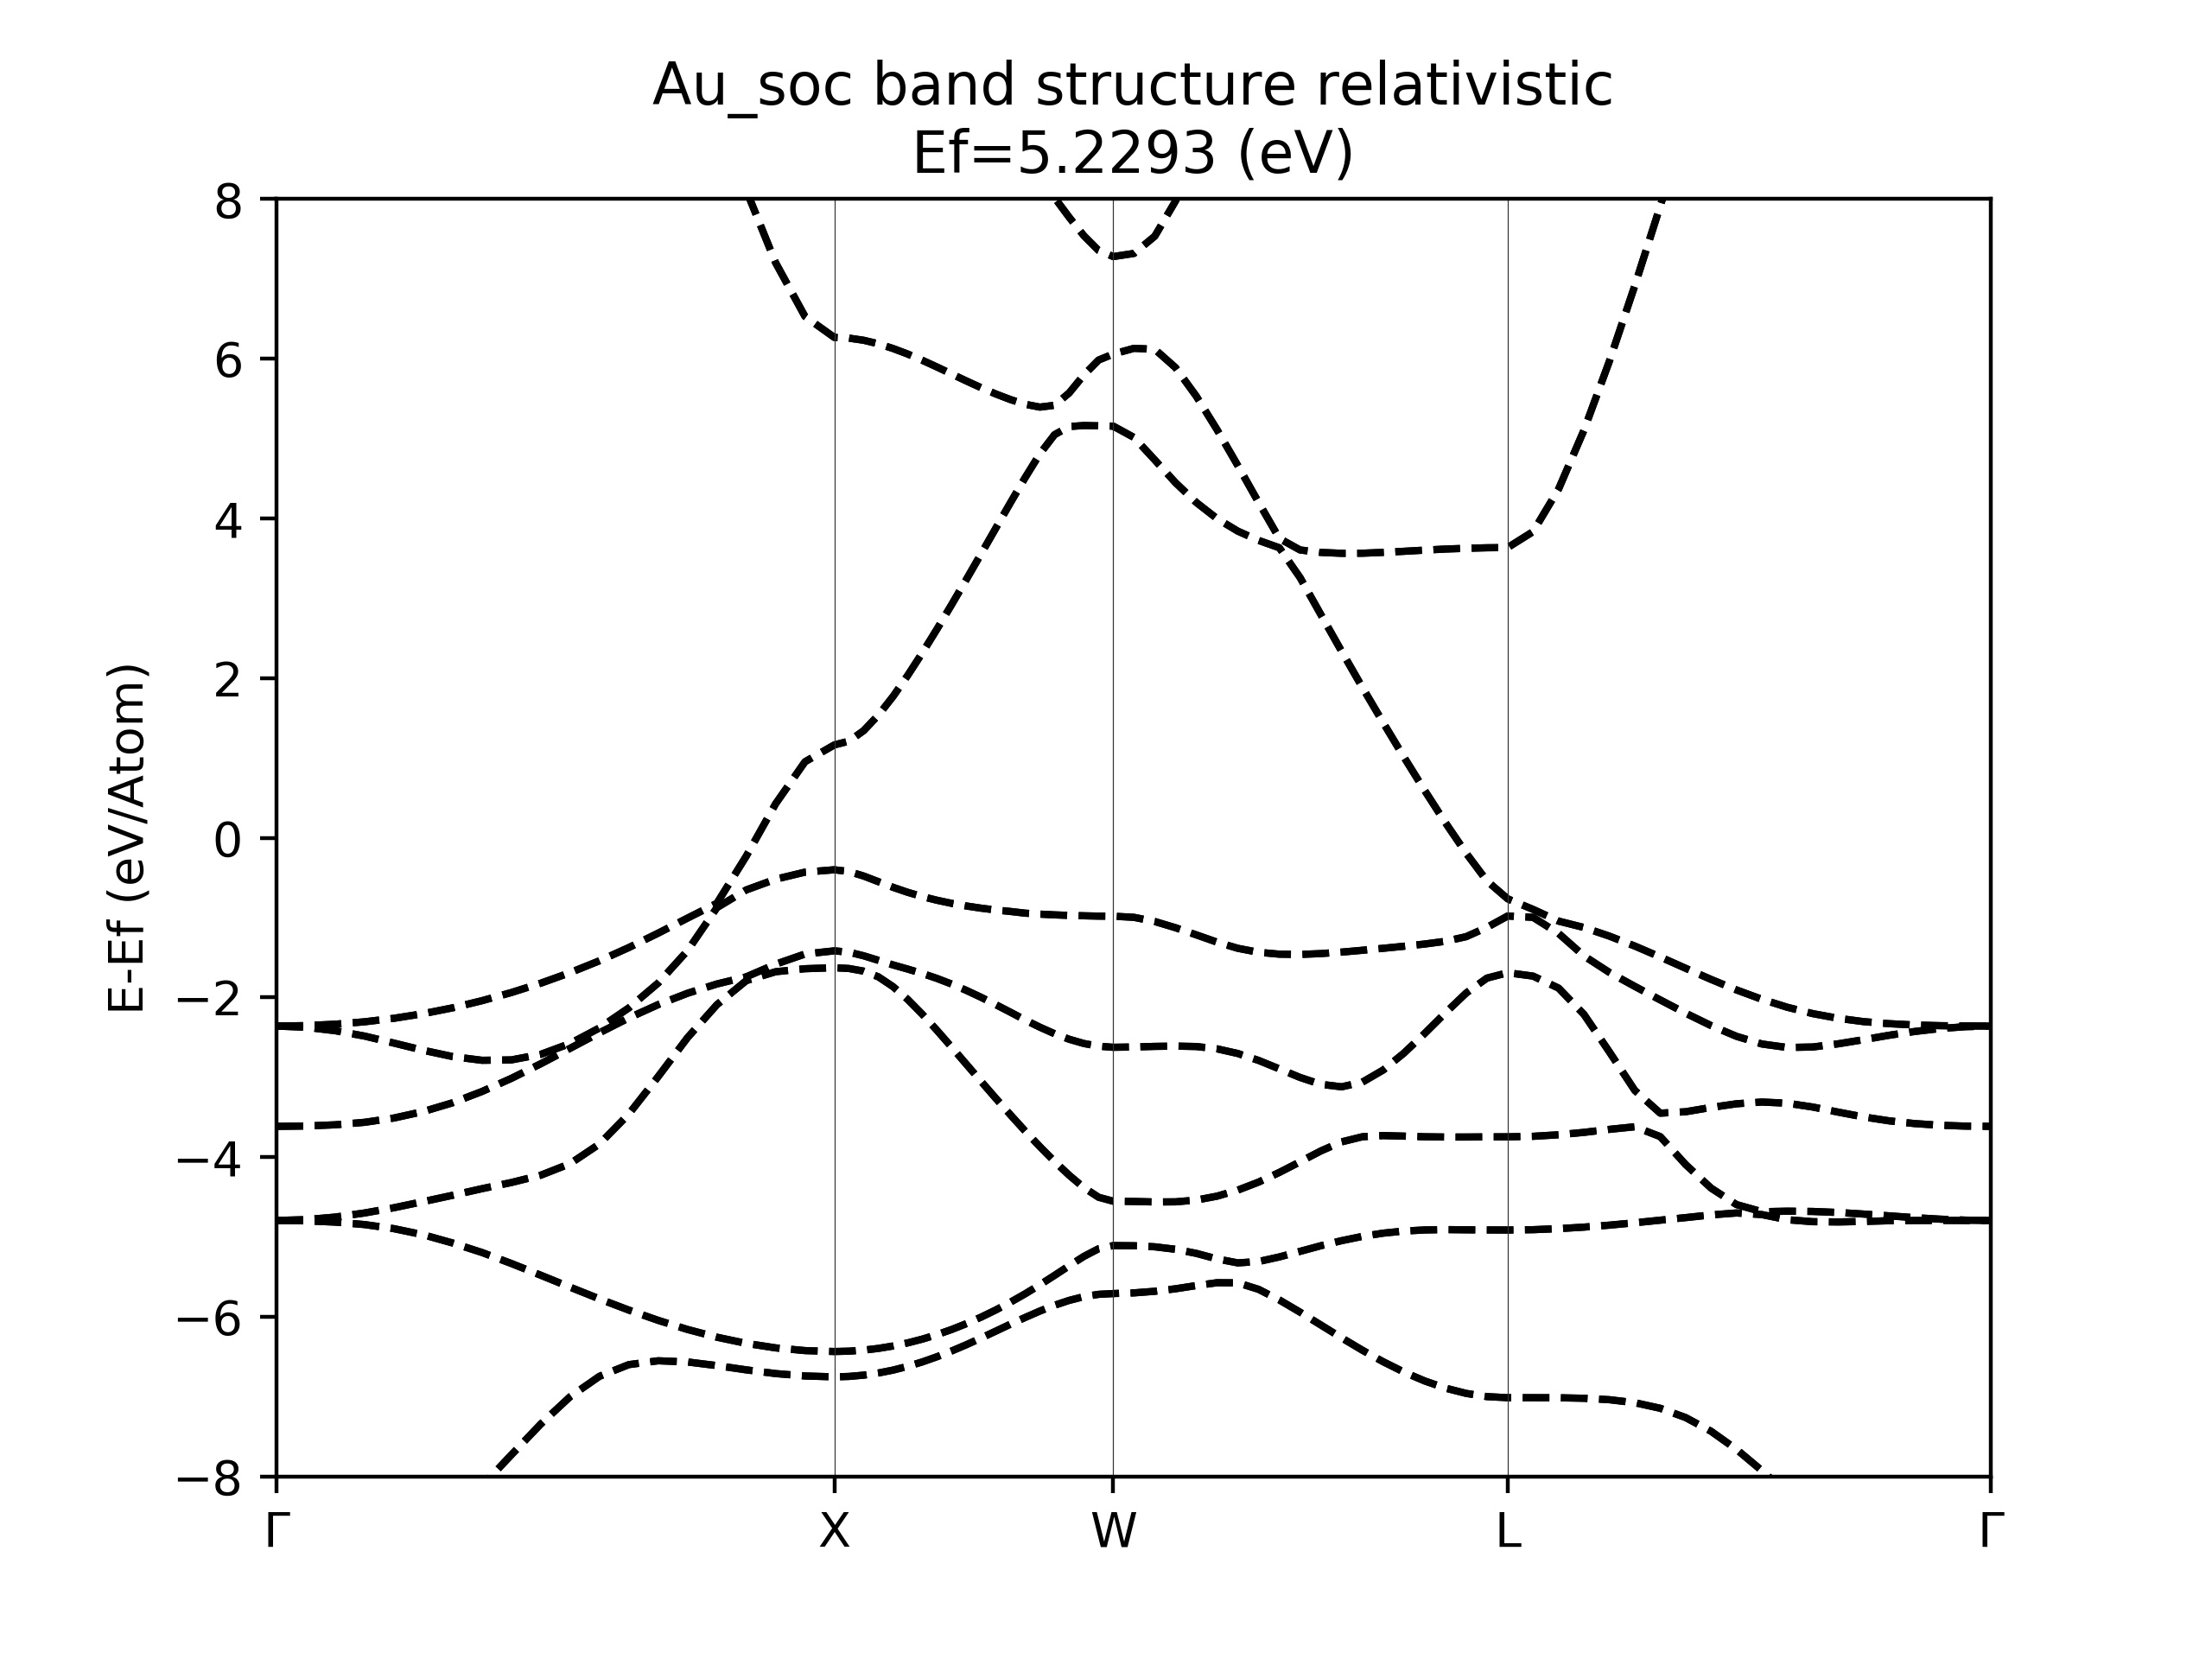
\includegraphics[width=\textwidth]{{data/q2/All_Data/Au_data/Au_soc}.jpg}
					\caption{Au band structure with SOC}
					\label{fig:Ausocband}
				\end{minipage}
				\begin{minipage}[b]{0.45\textwidth}
					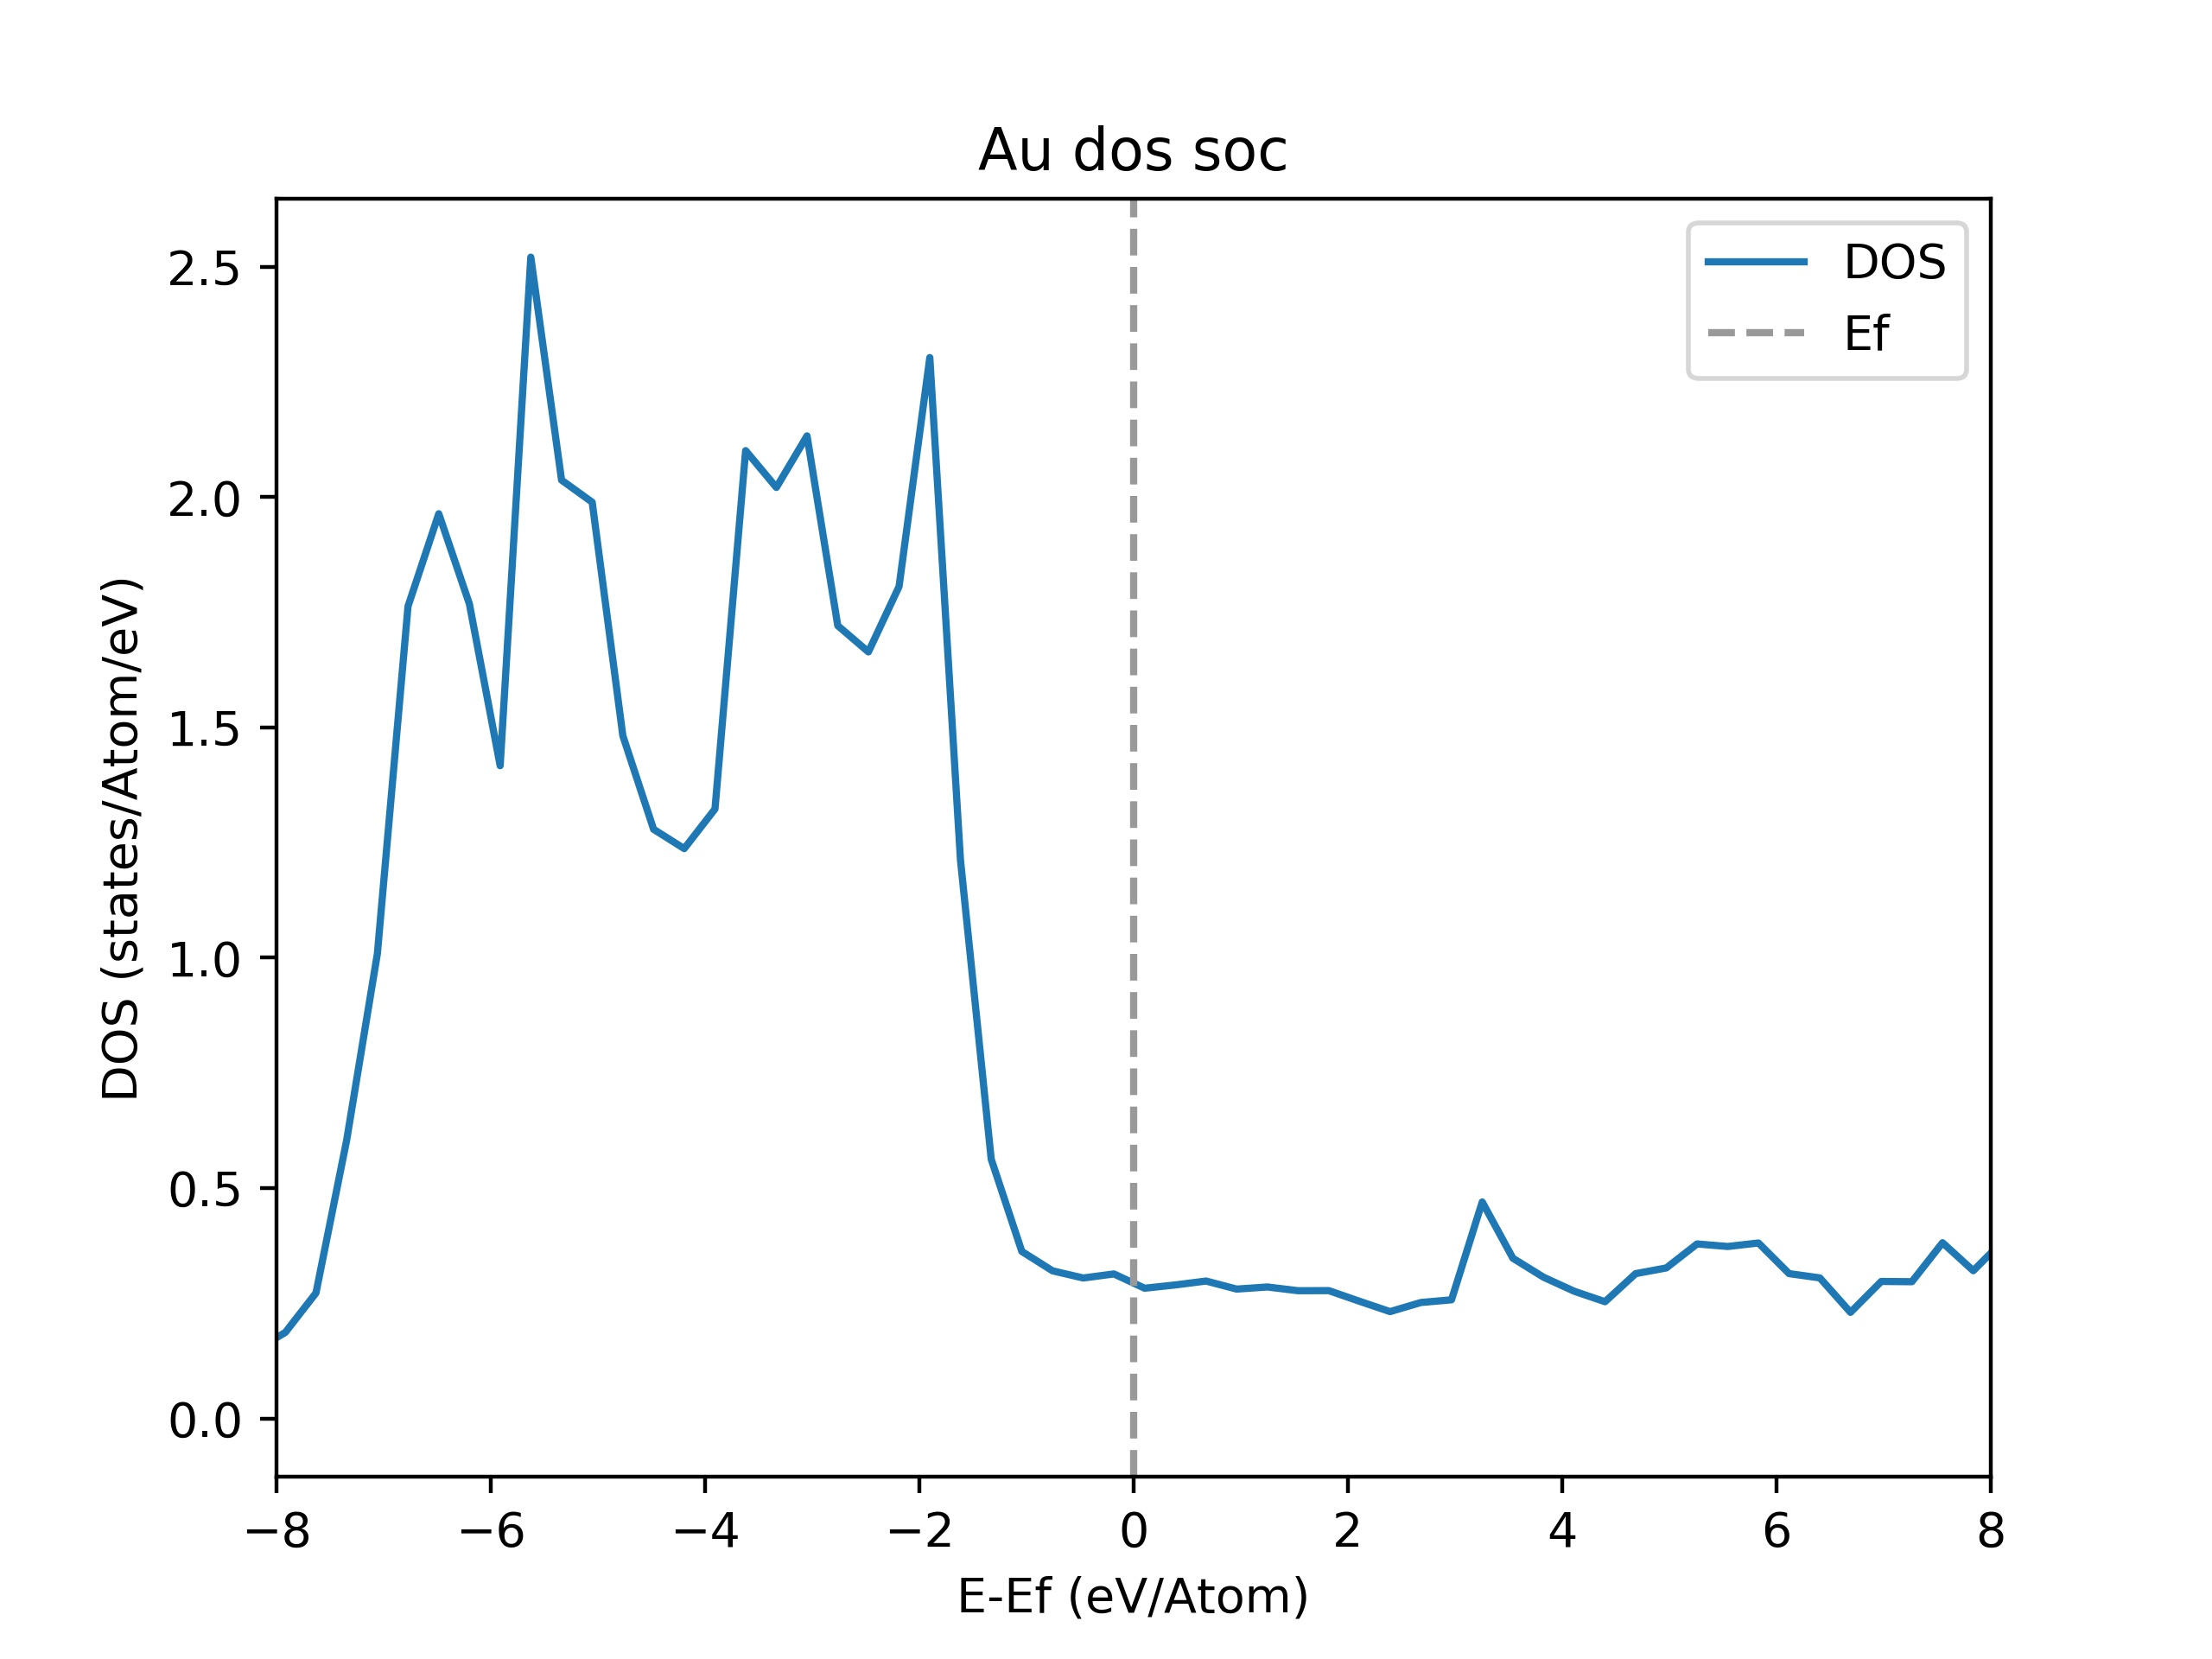
\includegraphics[width=\textwidth]{{data/q2/All_Data/Au_data/Au_soc_dos}.jpg}
					\caption{Au DOS with SOC}
					\label{fig:Ausocdos}
				\end{minipage}
				\begin{minipage}[b]{0.45\textwidth}
					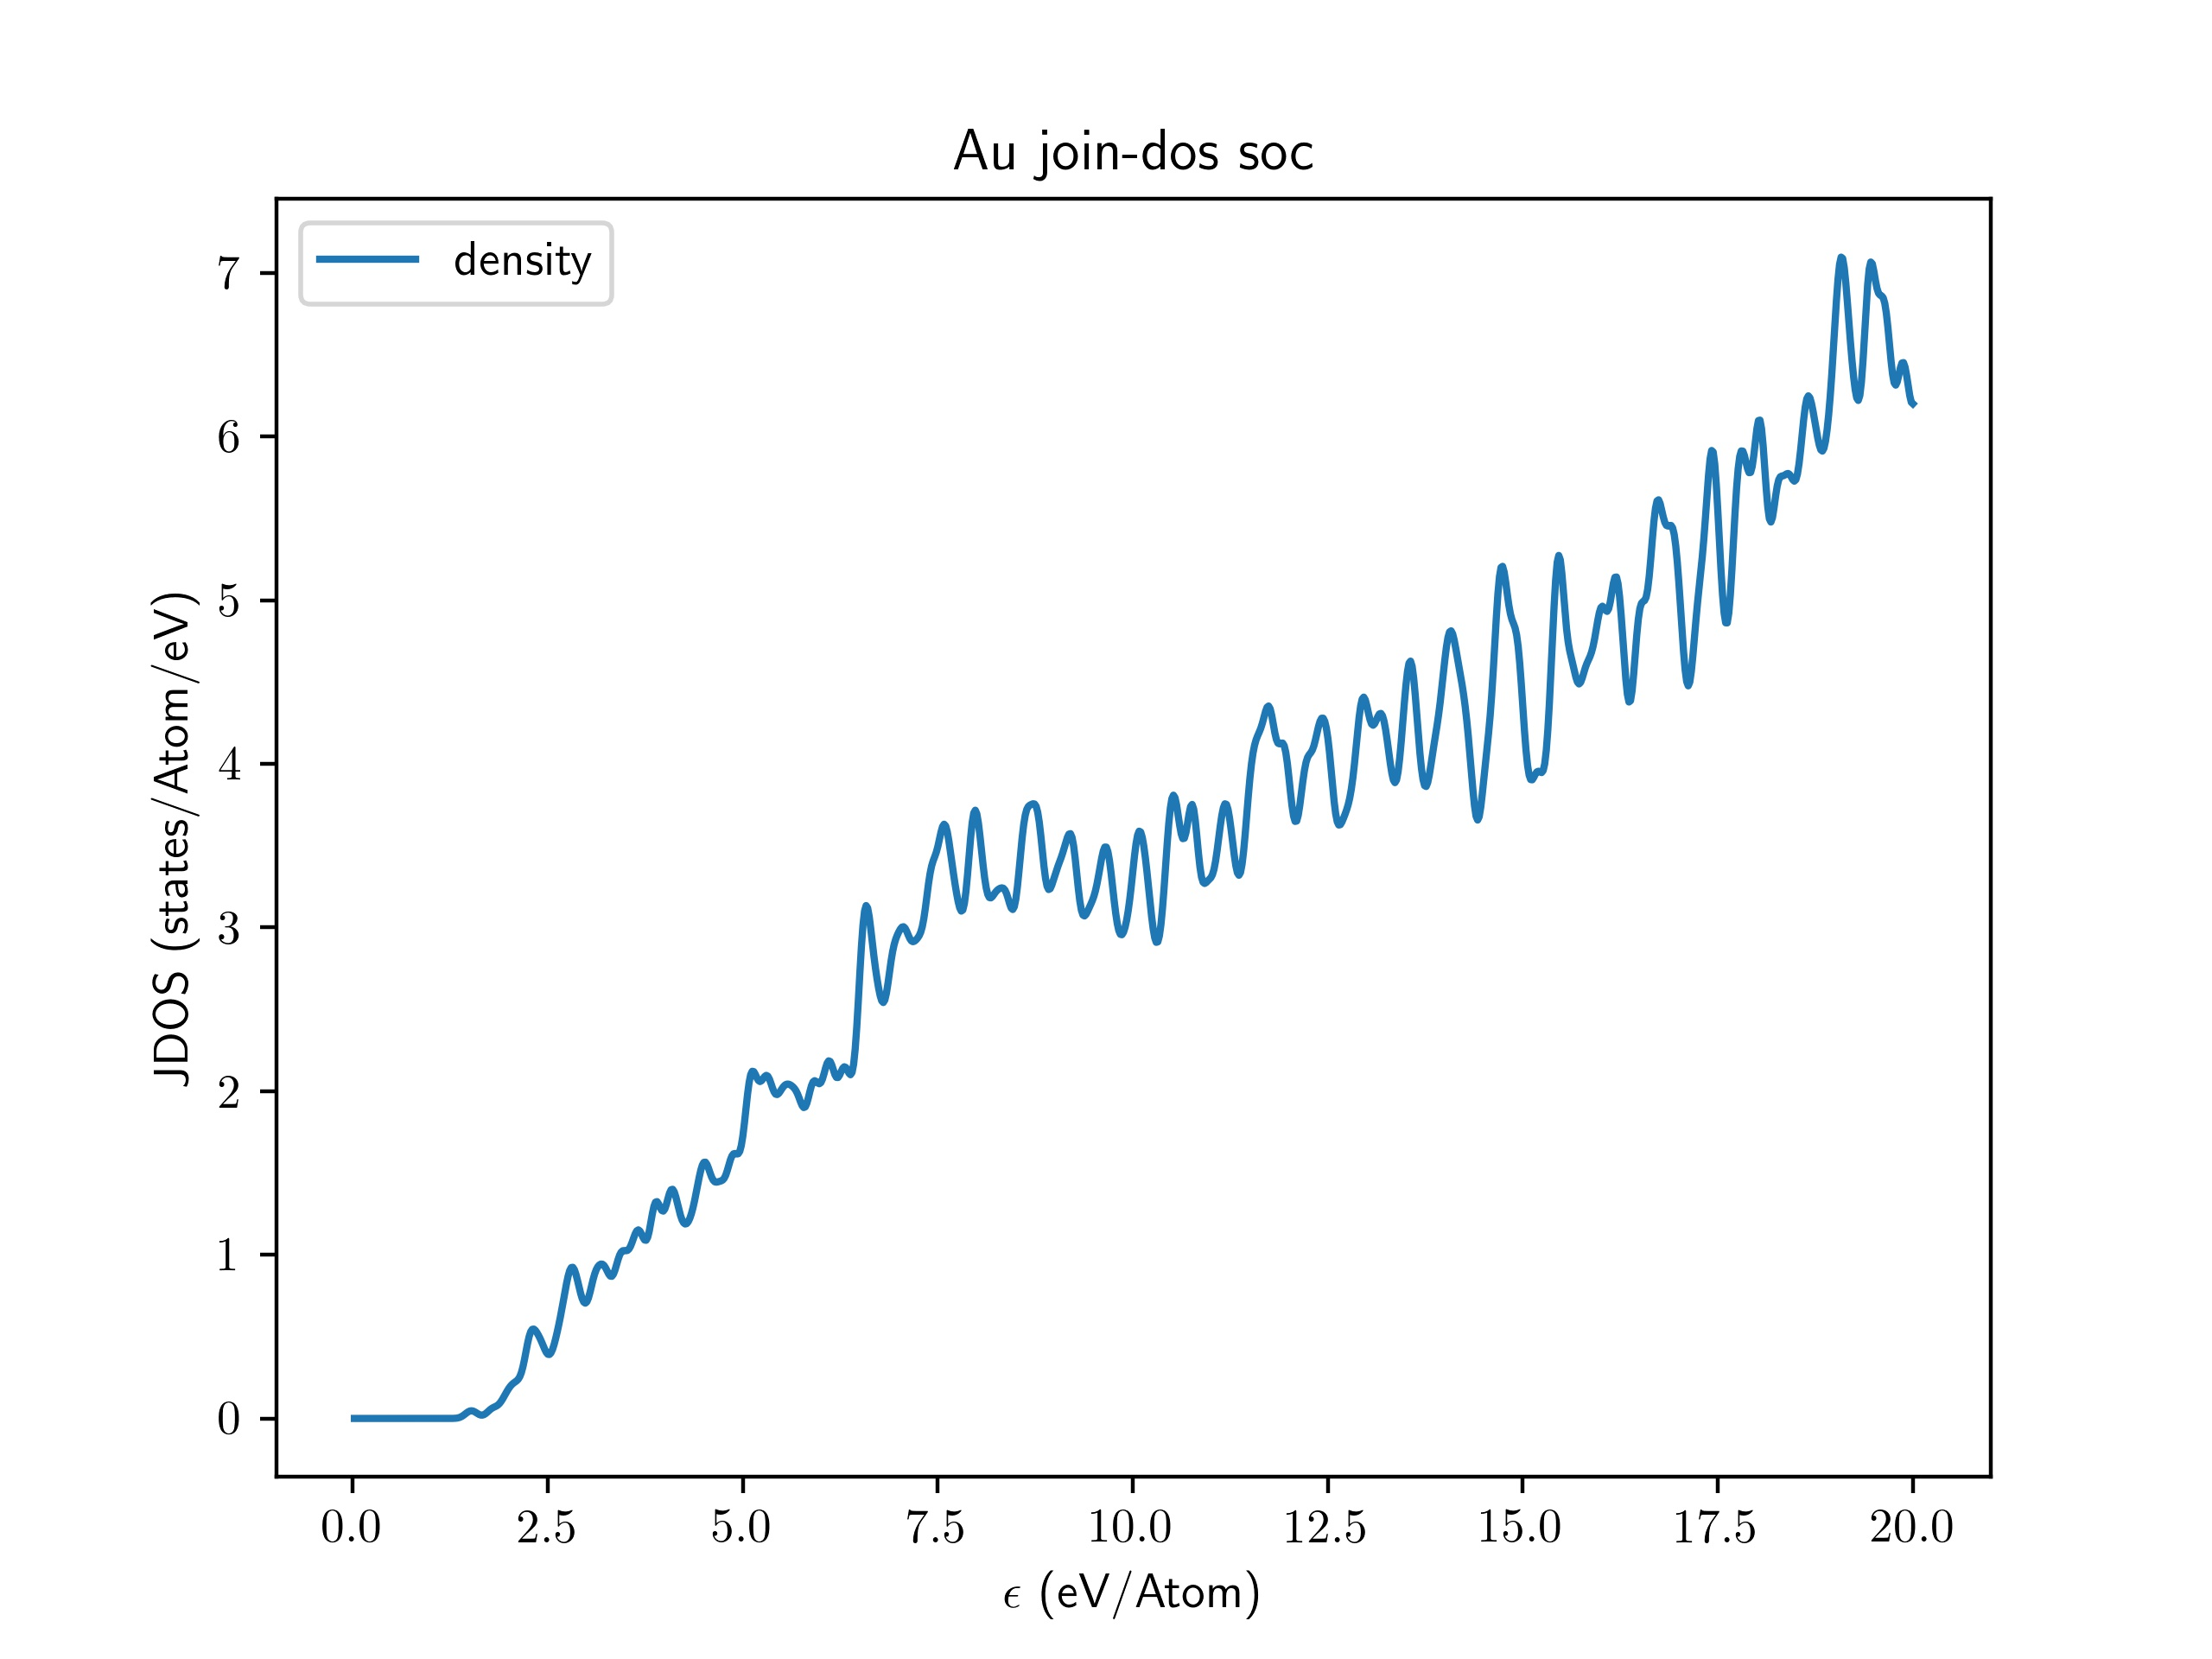
\includegraphics[width=\textwidth]{{data/q2/All_Data/Au_data/Au_soc_jdos}.jpg}
					\caption{Au join-DOS with SOC}
					\label{fig:Ausocjdos}
				\end{minipage}
				\begin{minipage}[b]{0.45\textwidth}
					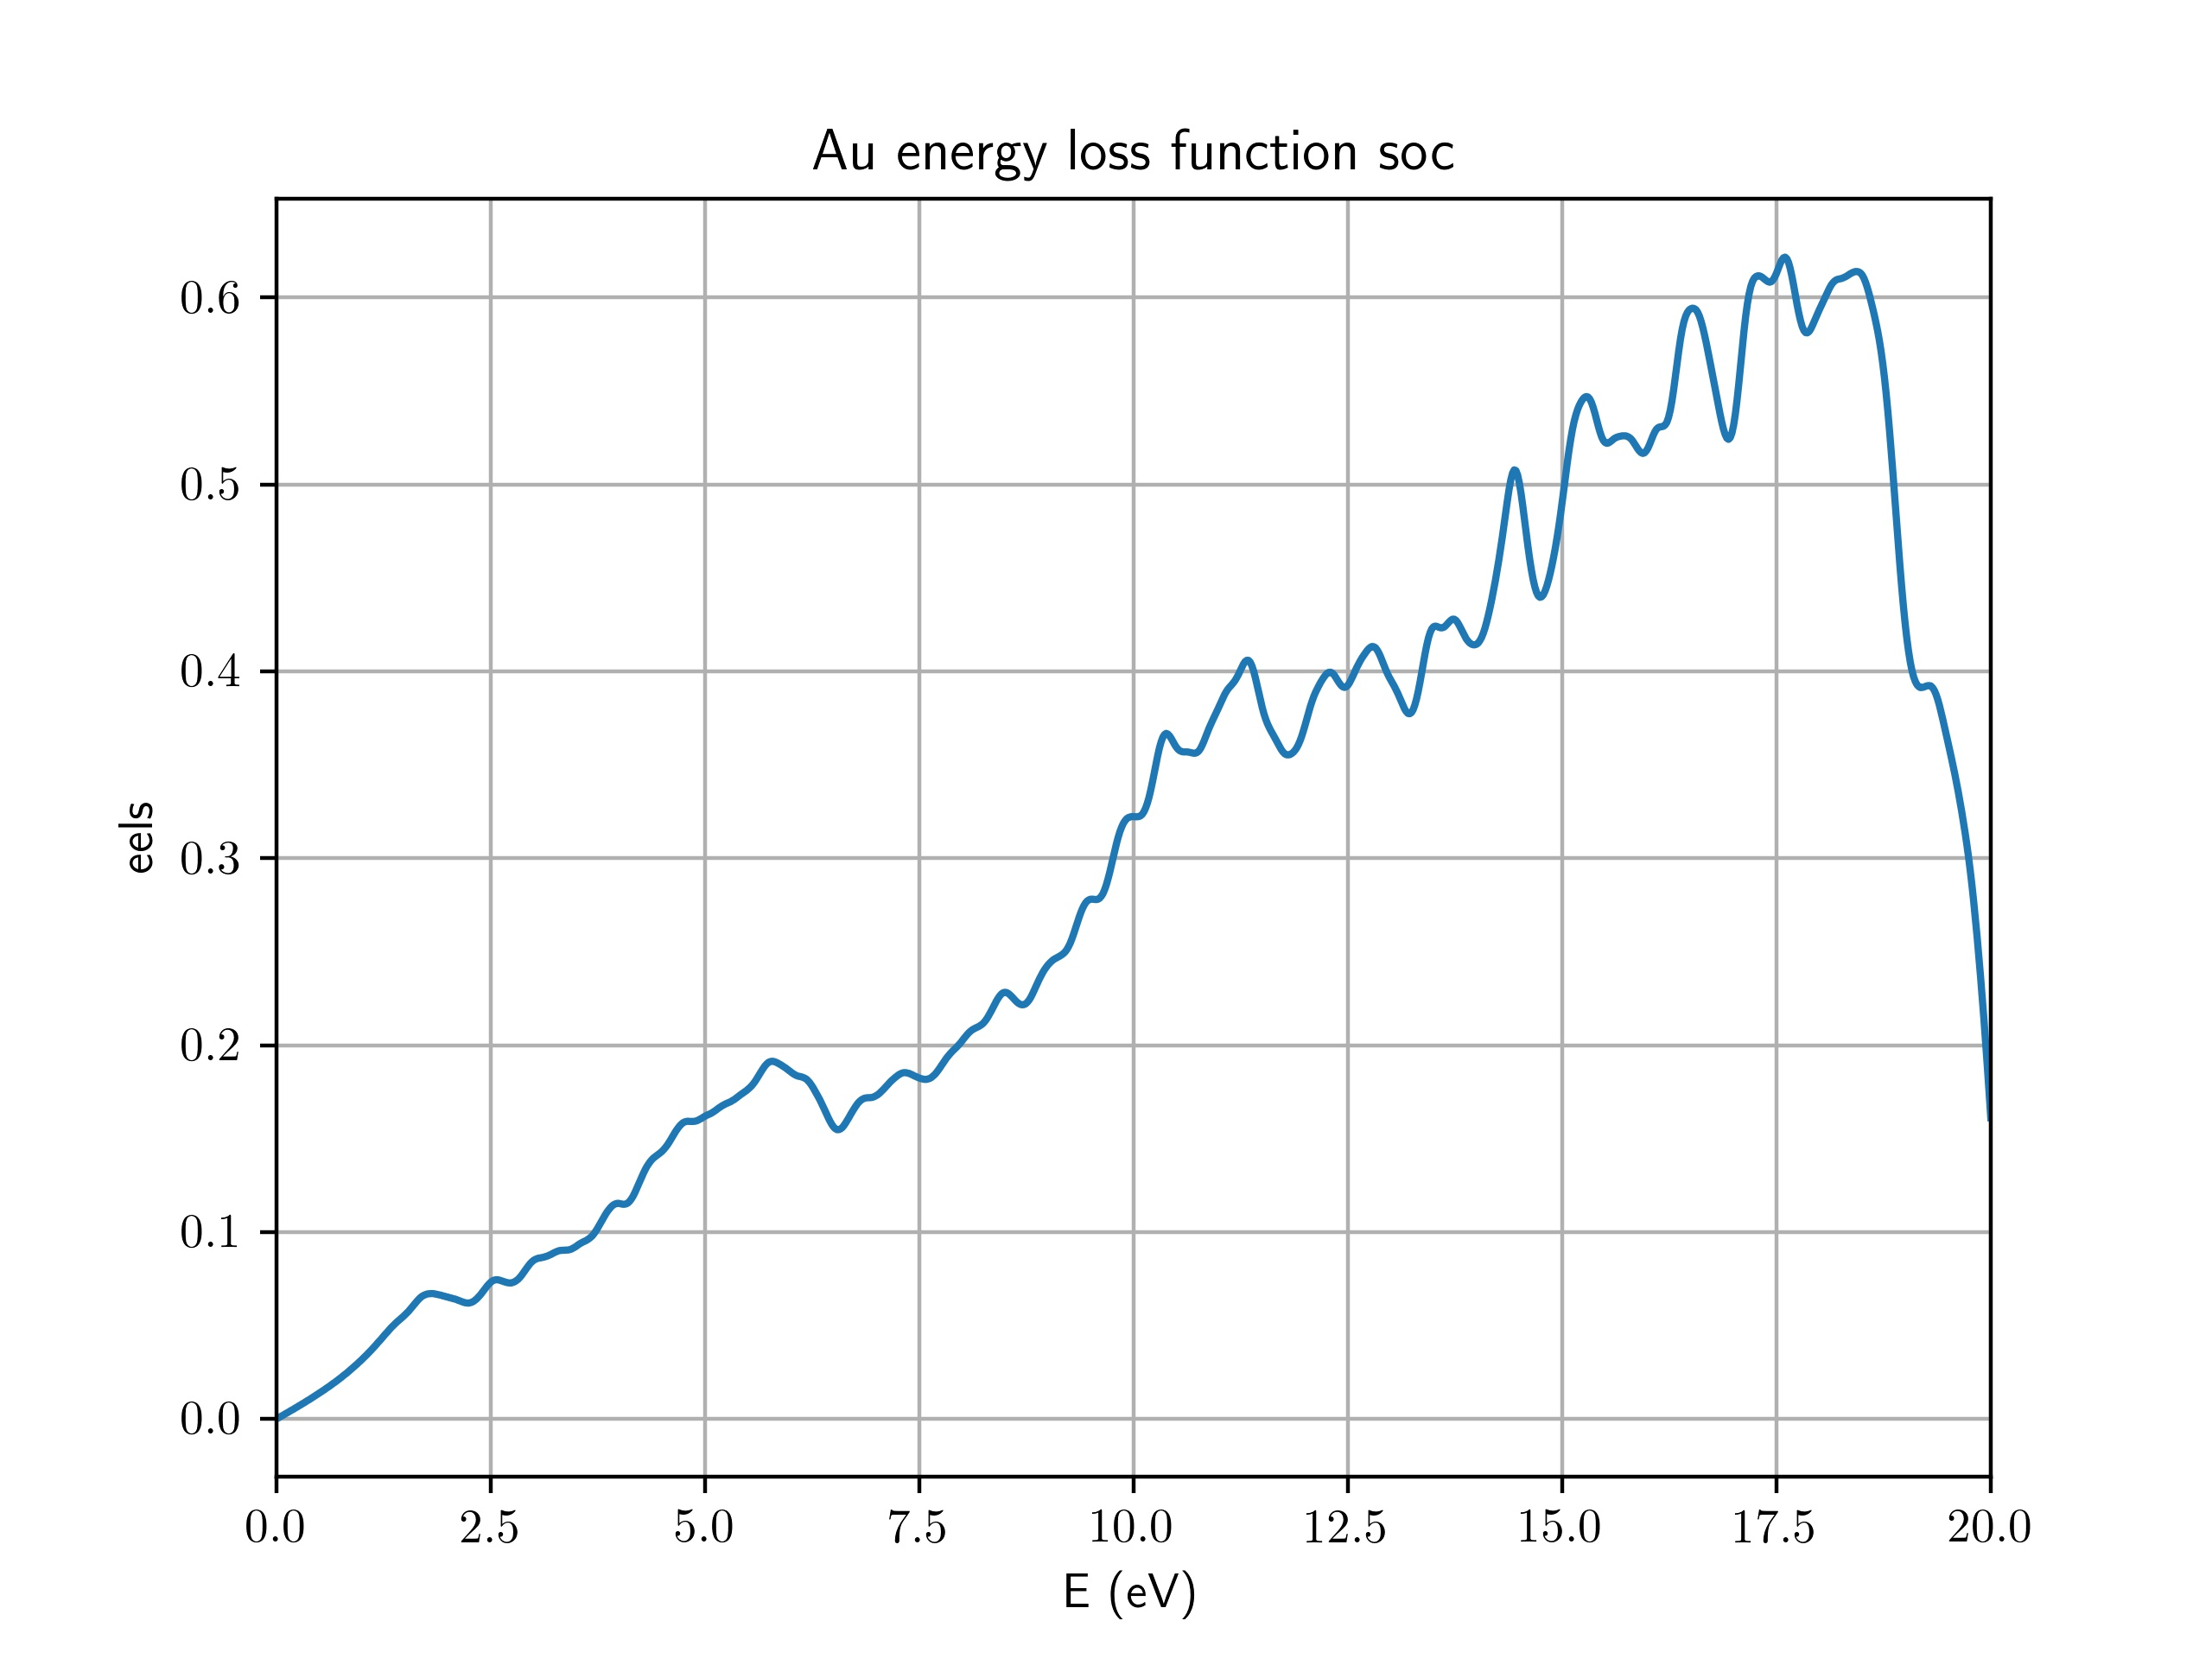
\includegraphics[width=\textwidth]{{data/q2/All_Data/Au_data/Au_soc_eels}.jpg}
					\caption{Au energy loss function with SOC}
					\label{fig:Ausoceels}
				\end{minipage}
			
			\end{figure} 
			\begin{figure}[h!]
				\begin{minipage}[b]{0.45\textwidth}
					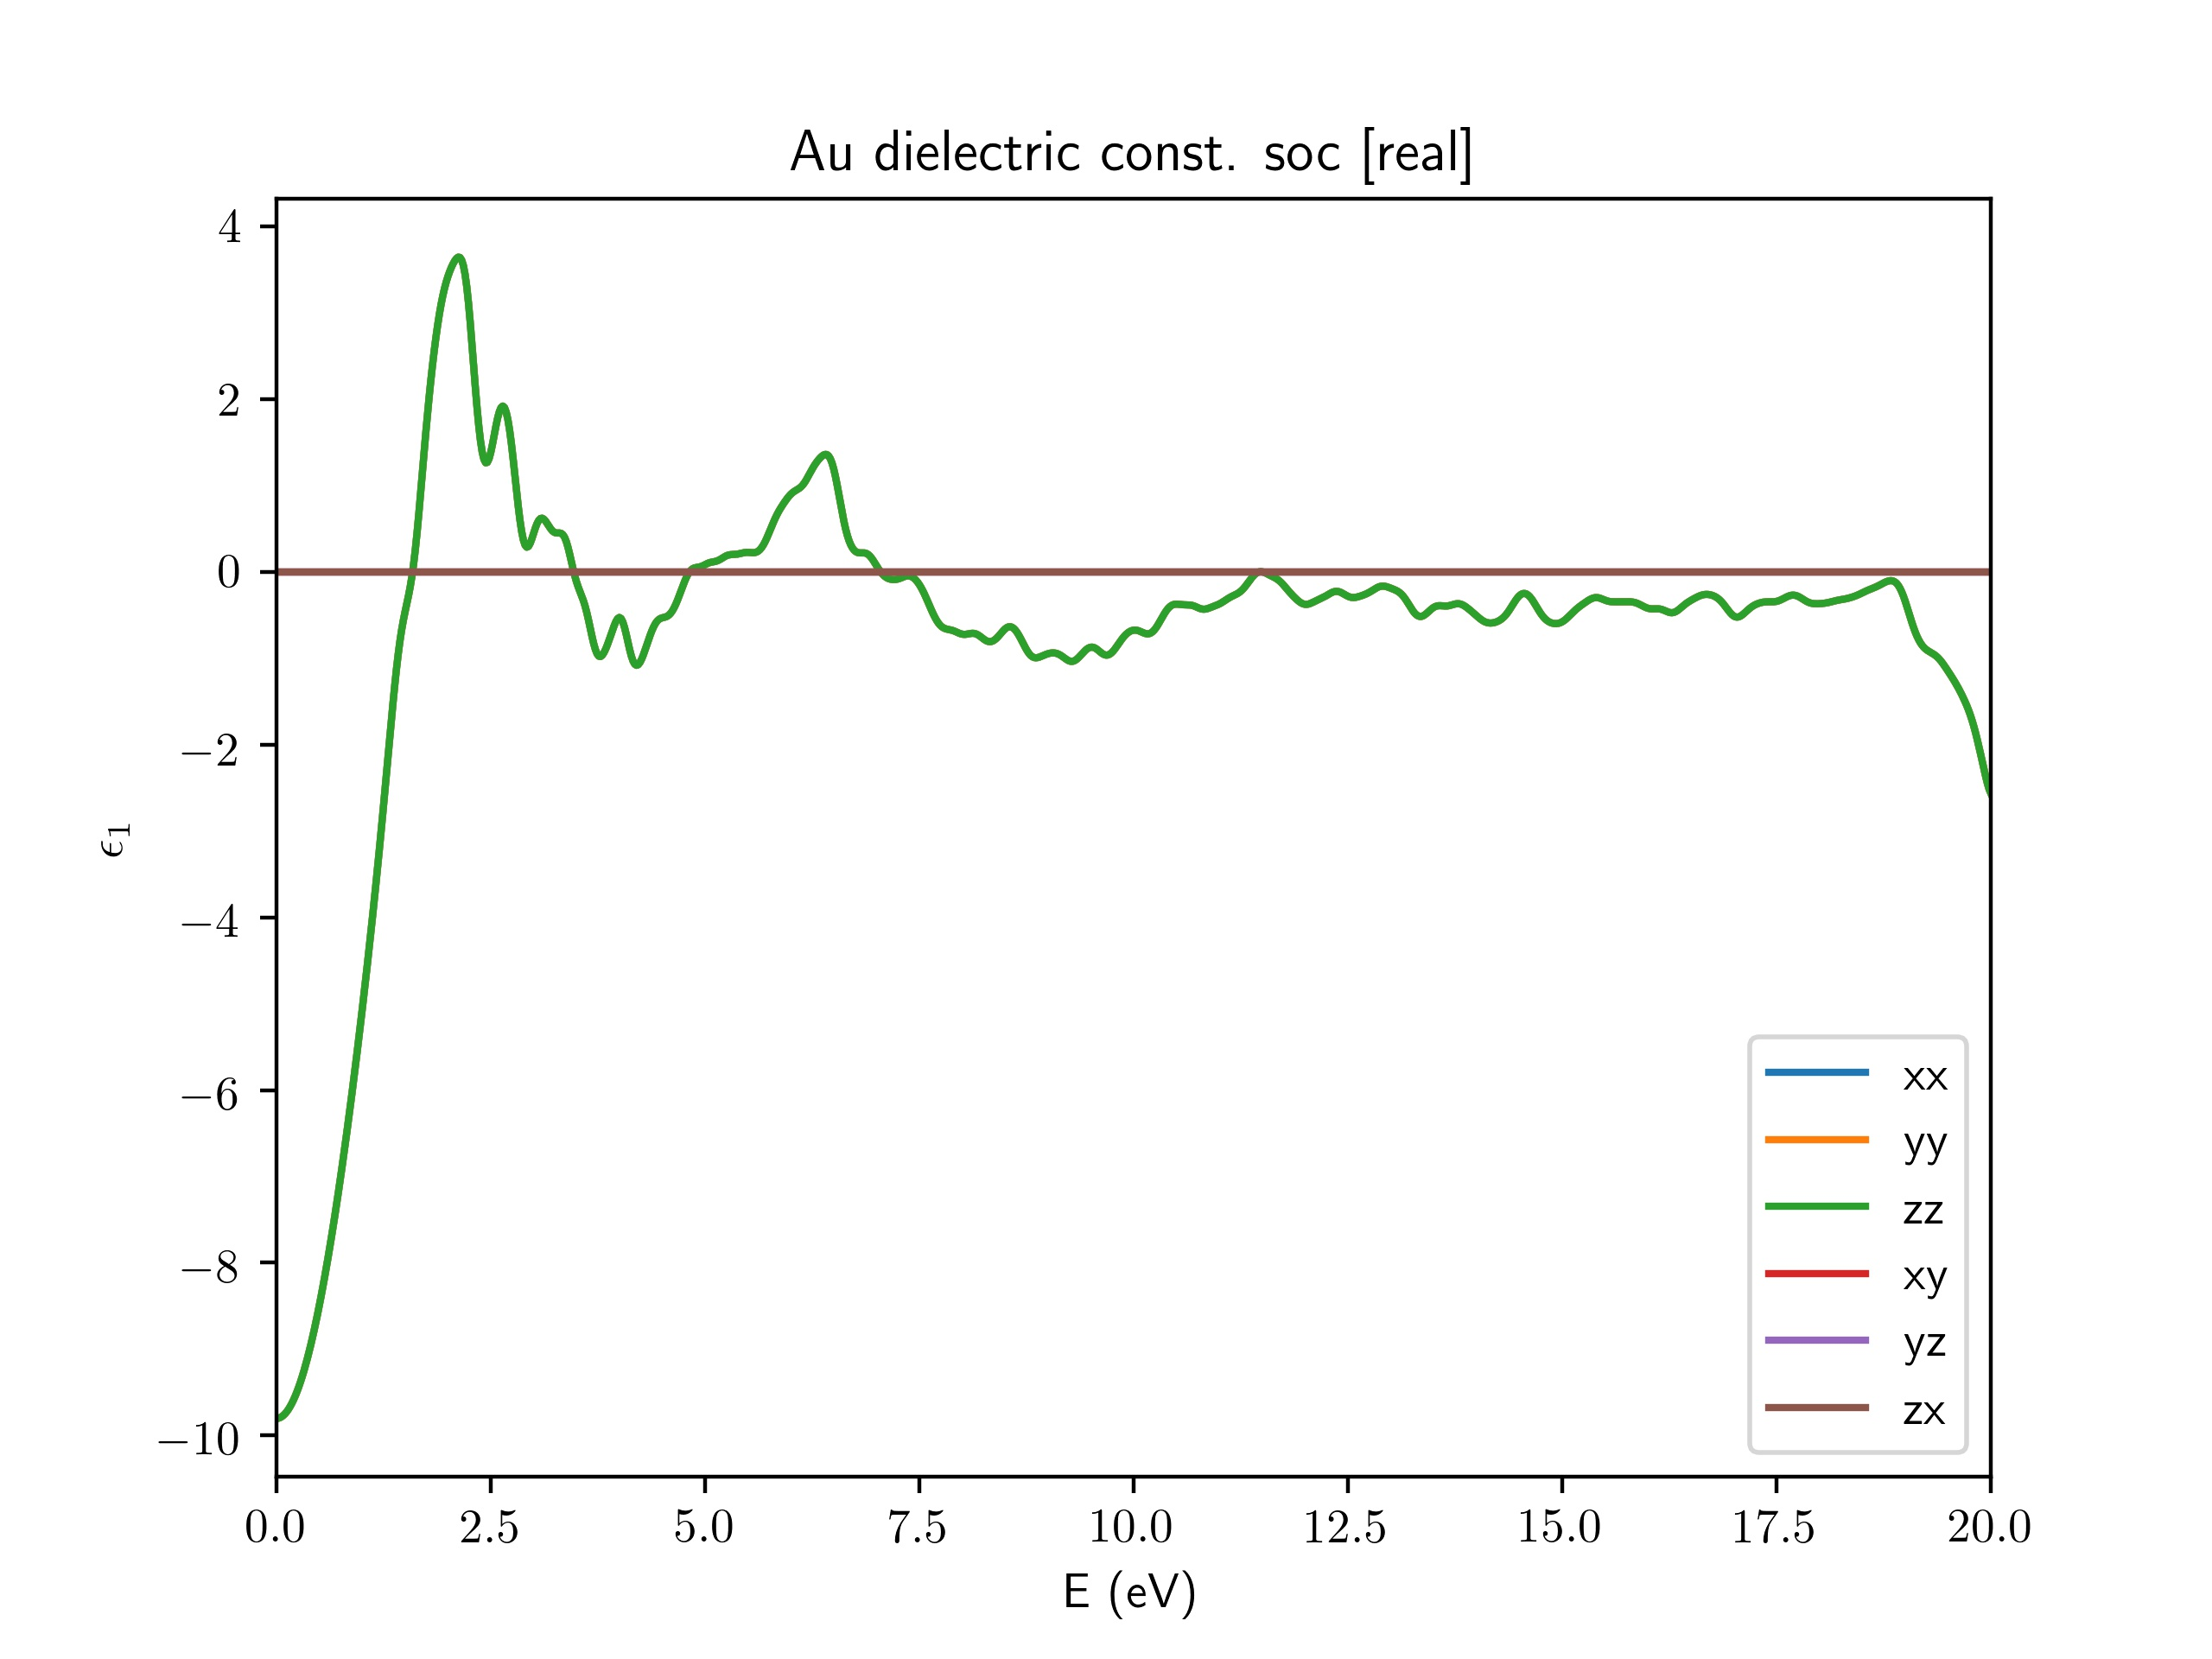
\includegraphics[width=\textwidth]{{data/q2/All_Data/Au_data/Au_soc_epsre}.jpg}
					\caption{Au dielectric constant (real) with SOC}
					\label{fig:Ausocepsre}
				\end{minipage}
				\begin{minipage}[b]{0.45\textwidth}
					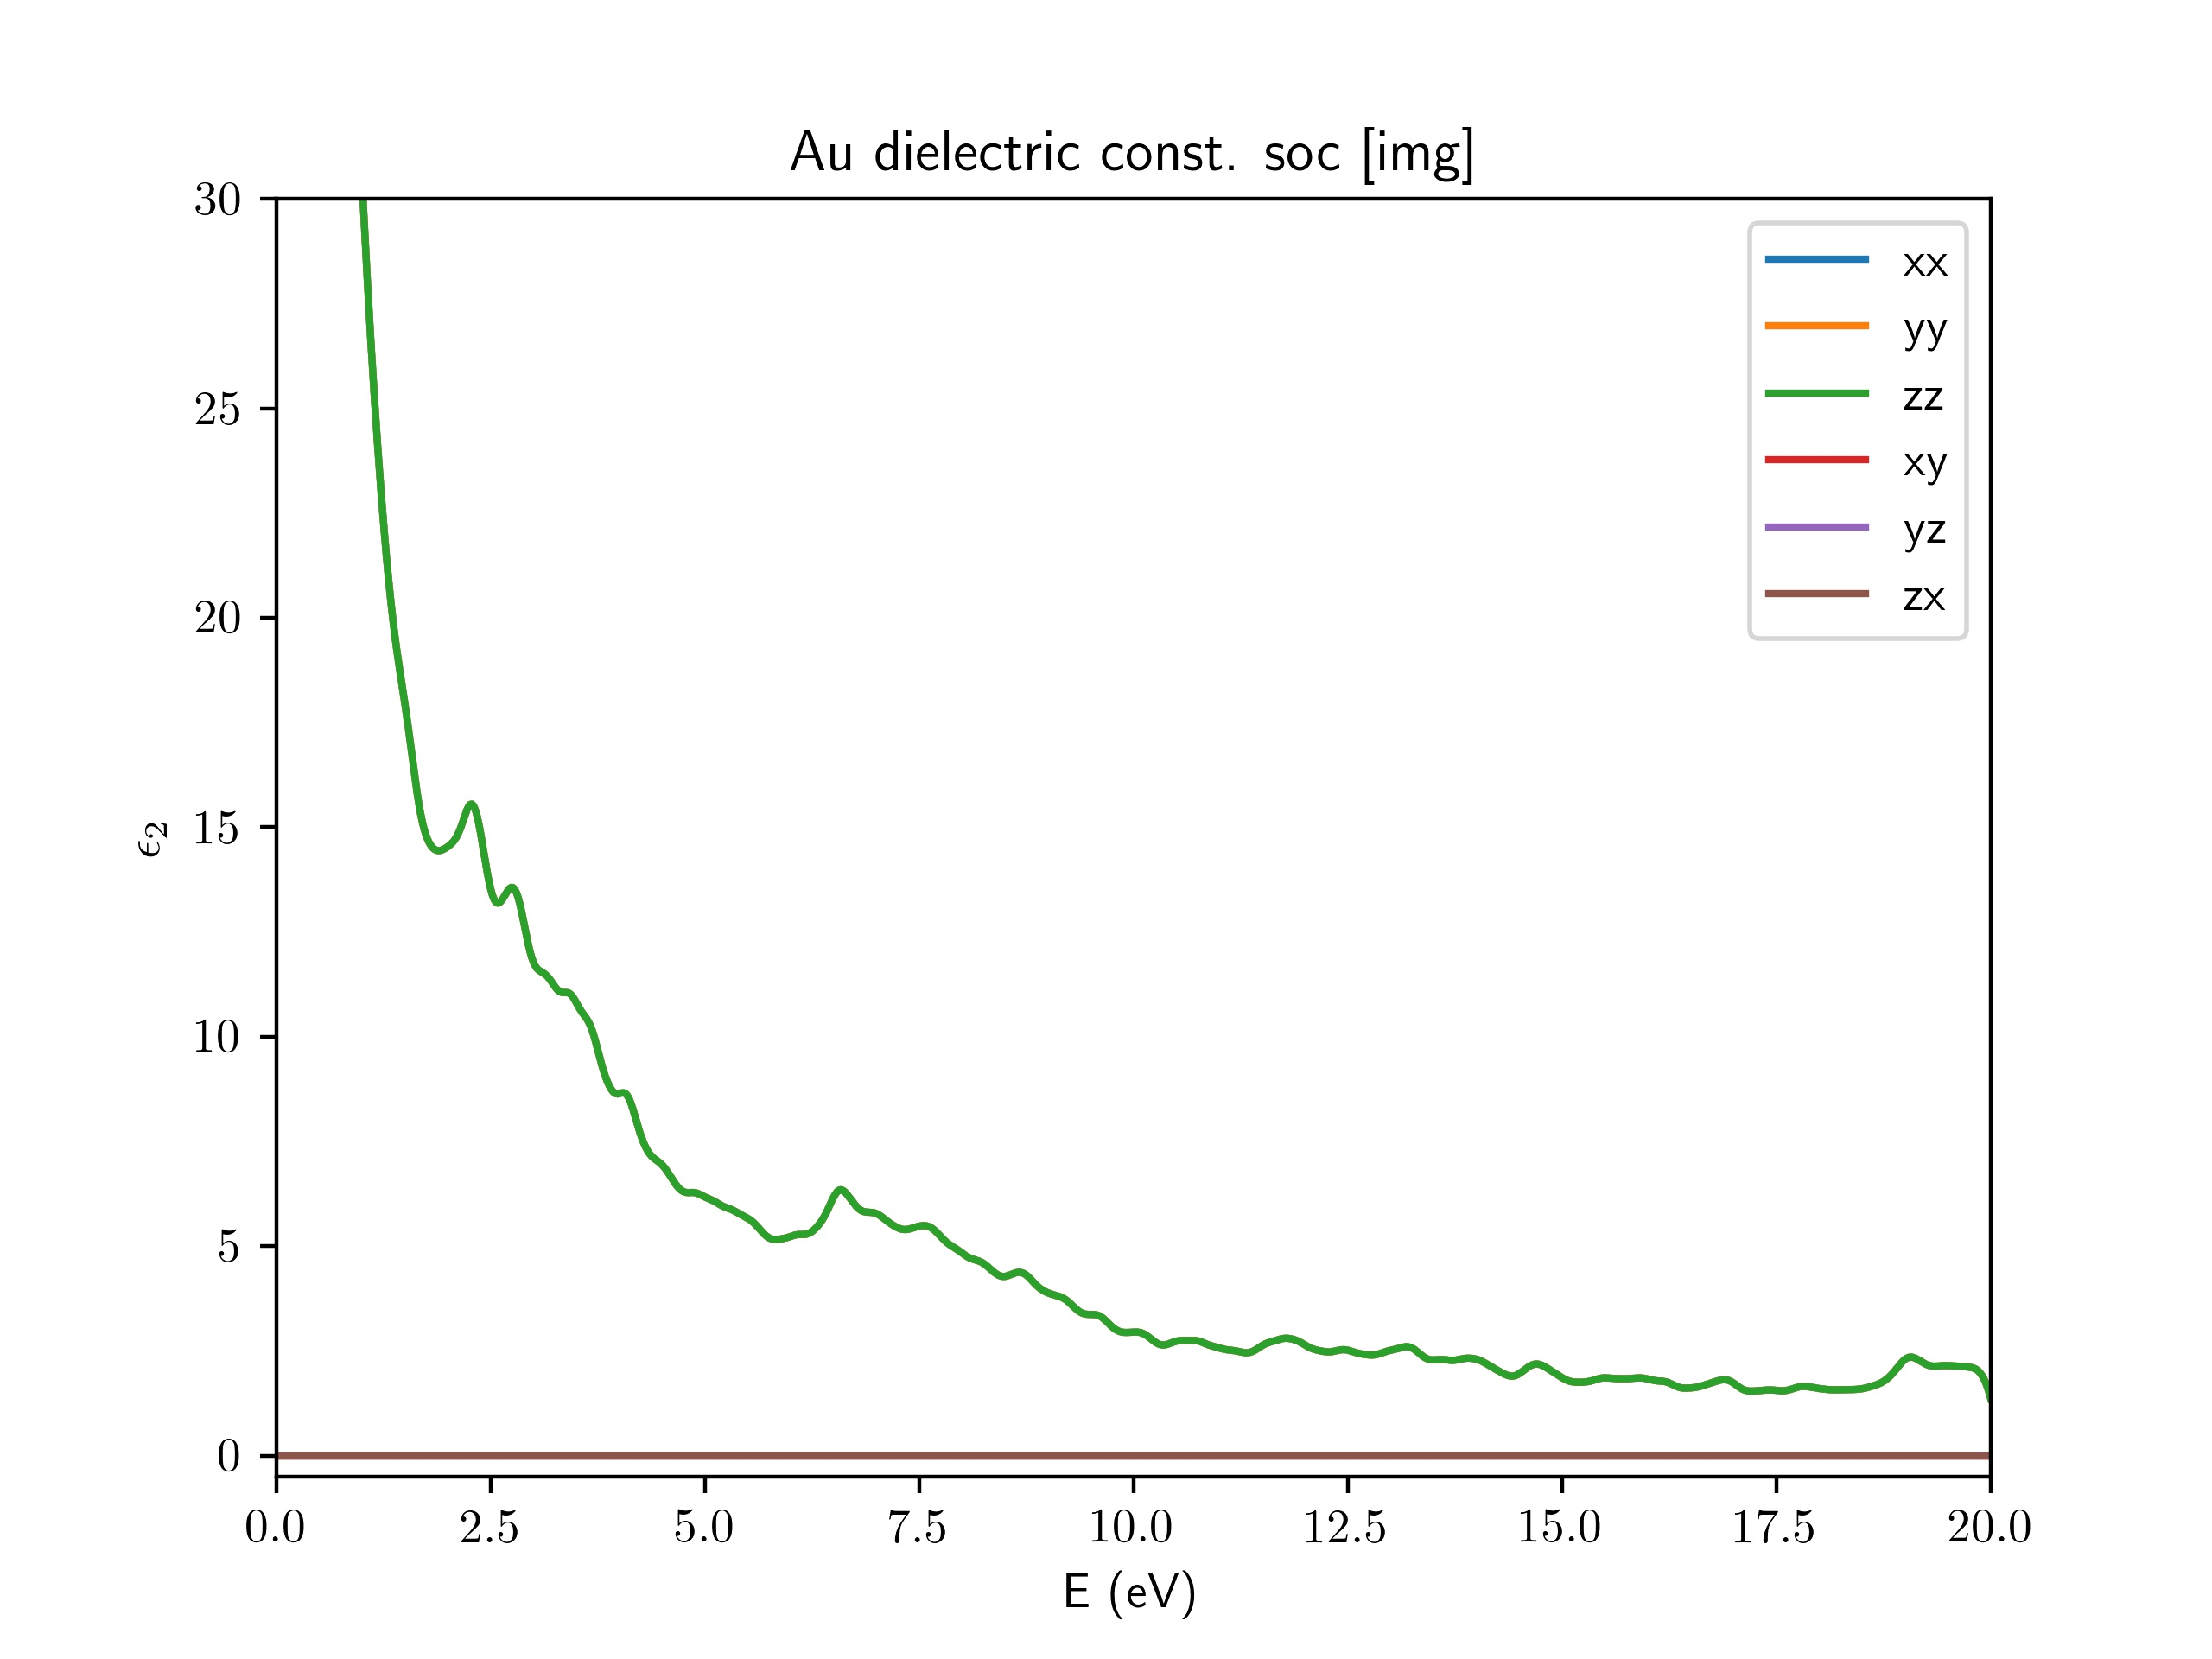
\includegraphics[width=\textwidth]{{data/q2/All_Data/Au_data/Au_soc_epsim}.jpg}
					\caption{Au dielectric constant (image) with SOC}
					\label{fig:Ausocepsim}
				\end{minipage}
				\begin{minipage}[b]{0.45\textwidth}
					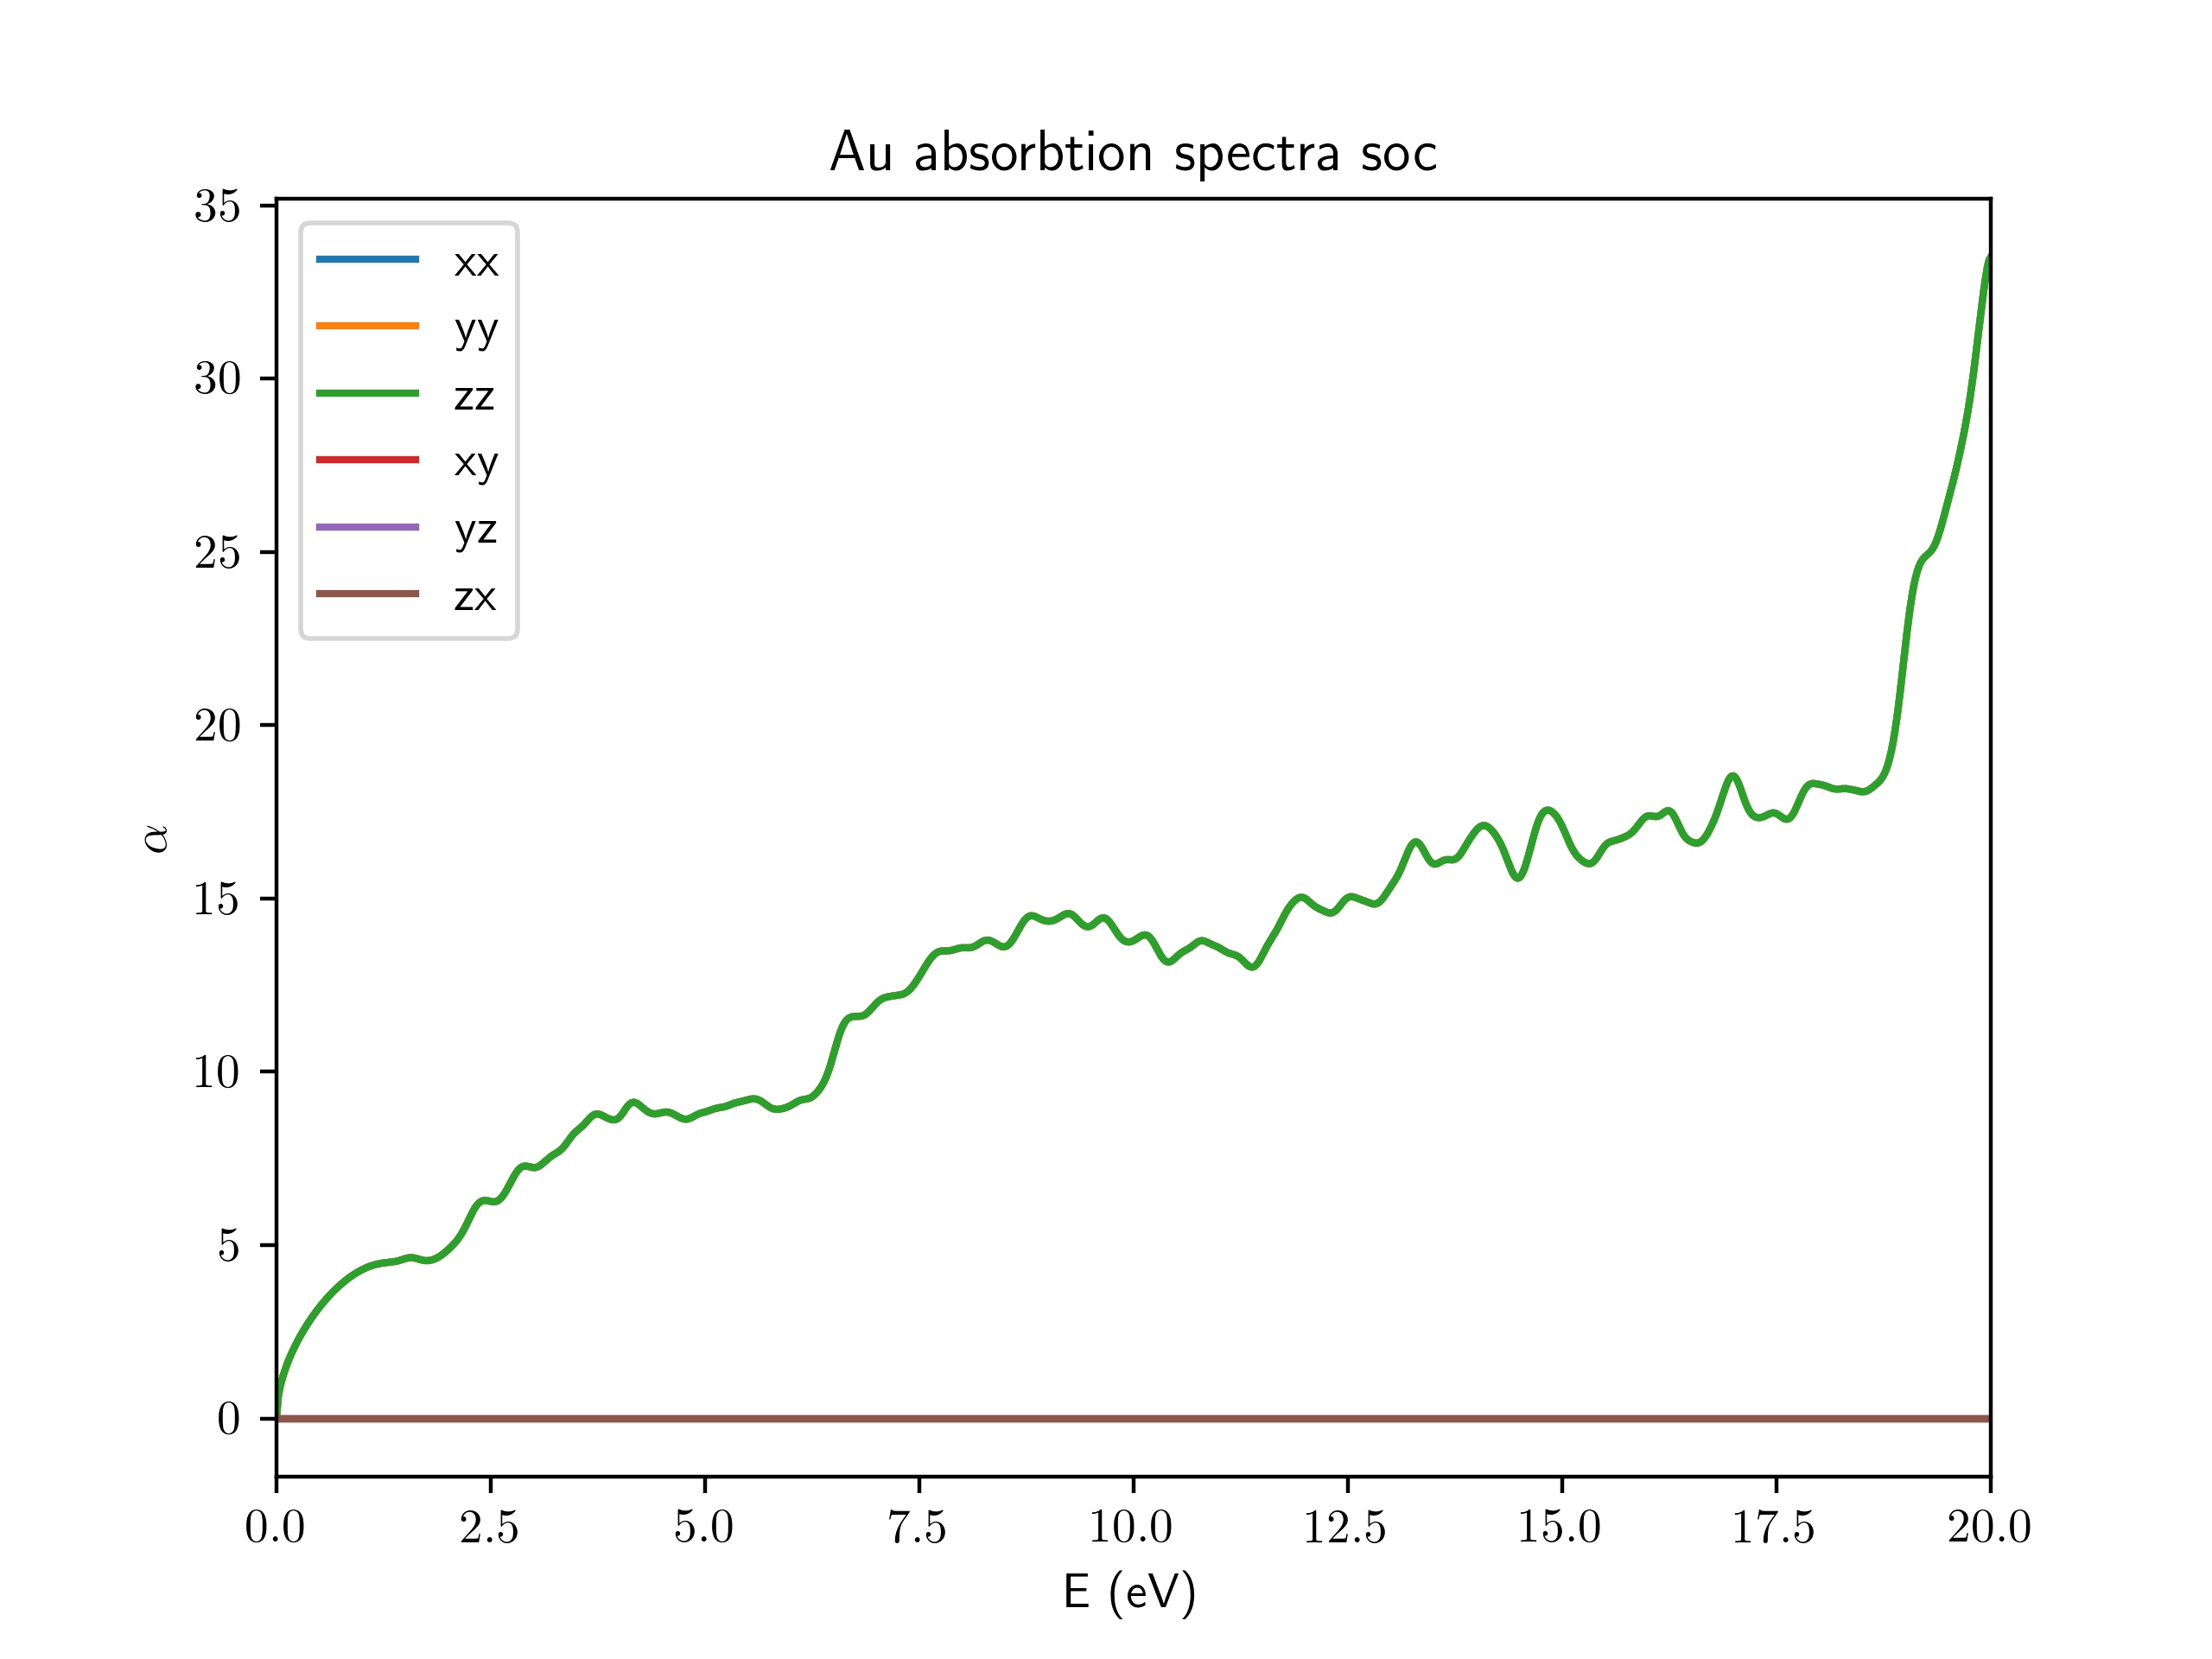
\includegraphics[width=\textwidth]{{data/q2/All_Data/Au_data/Au_soc_alpha}.jpg}
					\caption{Au absorption with SOC}
					\label{fig:Ausocalpha}
				\end{minipage}
			\end{figure} 

			\clearpage
			\item Si
			
			Following shows the bands structure, density of states for Si with spin orbital coupling (relativistic). Compare to Au, with the effect of spin-orbital coupling, the calculation results of Si doesn't differ much with non-relativistic calculation.  

			\begin{figure}[h!]
			
				\begin{minipage}[b]{0.45\textwidth}
					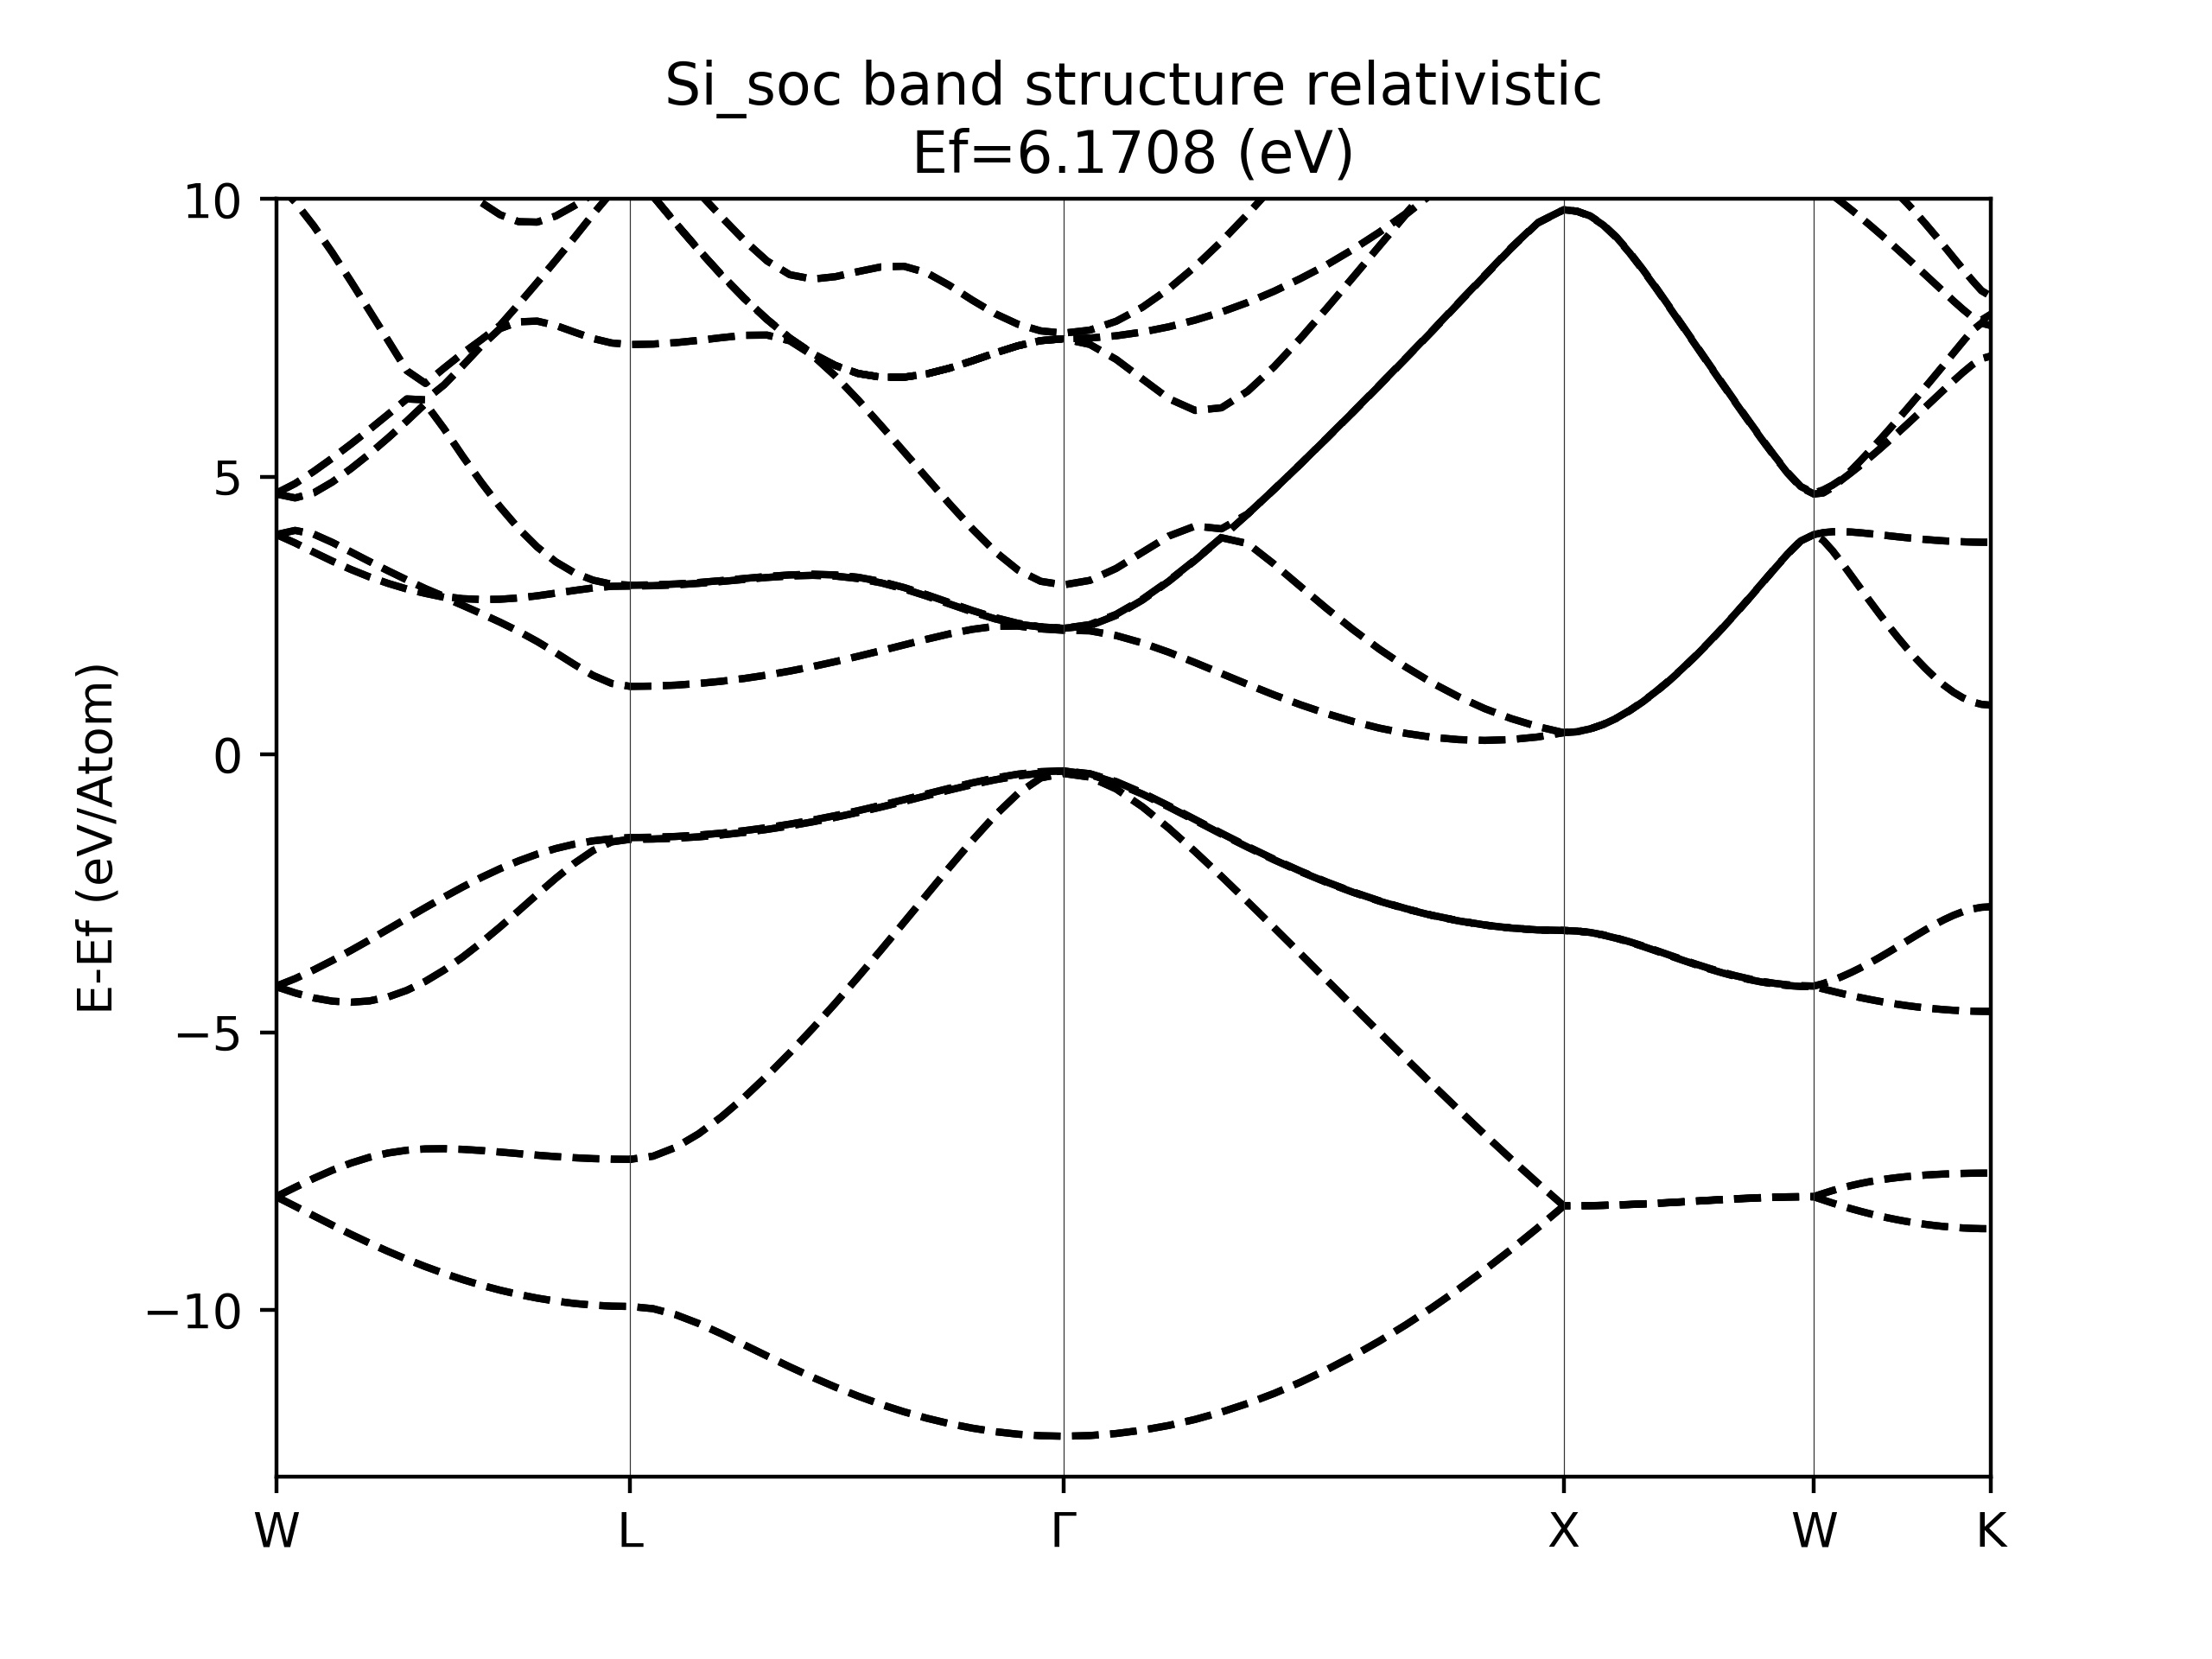
\includegraphics[width=\textwidth]{{data/q2/All_Data/Si_data/Si_soc}.jpg}
					\caption{Si band structure with SOC}
					\label{fig:Sisocband}
				\end{minipage}
				\begin{minipage}[b]{0.45\textwidth}
					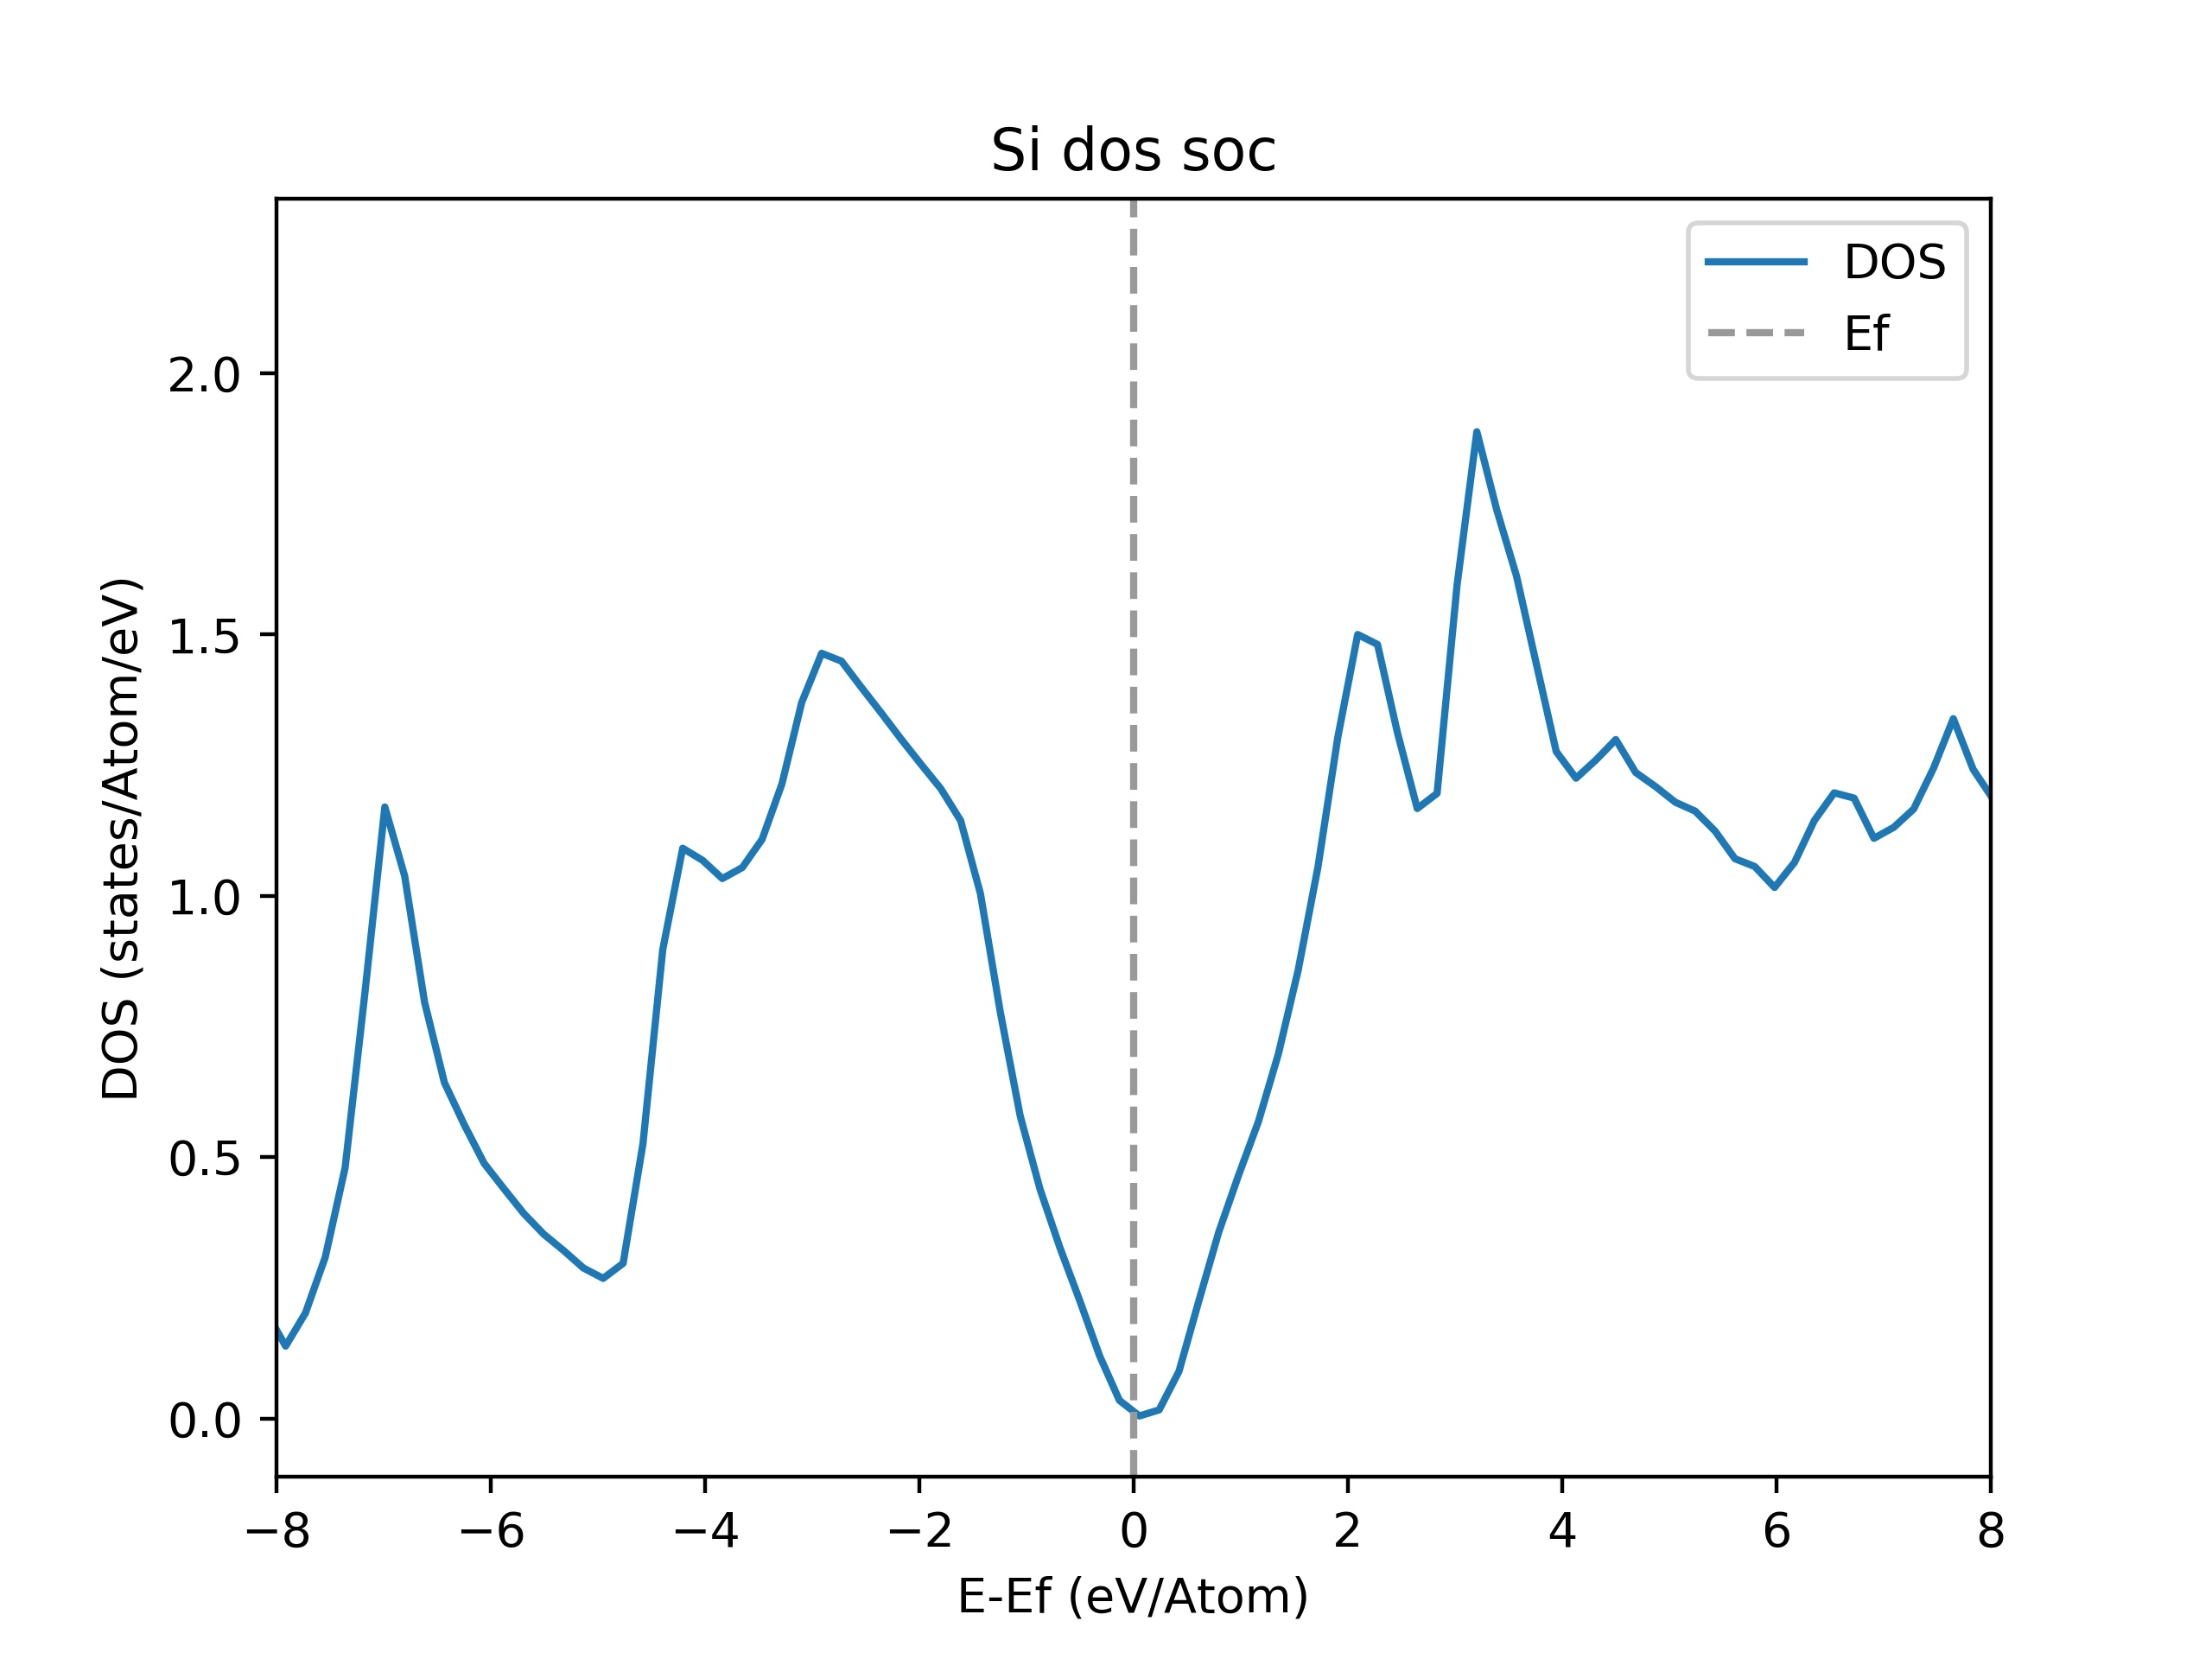
\includegraphics[width=\textwidth]{{data/q2/All_Data/Si_data/Si_soc_dos}.jpg}
					\caption{Si DOS with SOC}
					\label{fig:Sisocdos}
				\end{minipage}
				\begin{minipage}[b]{0.45\textwidth}
					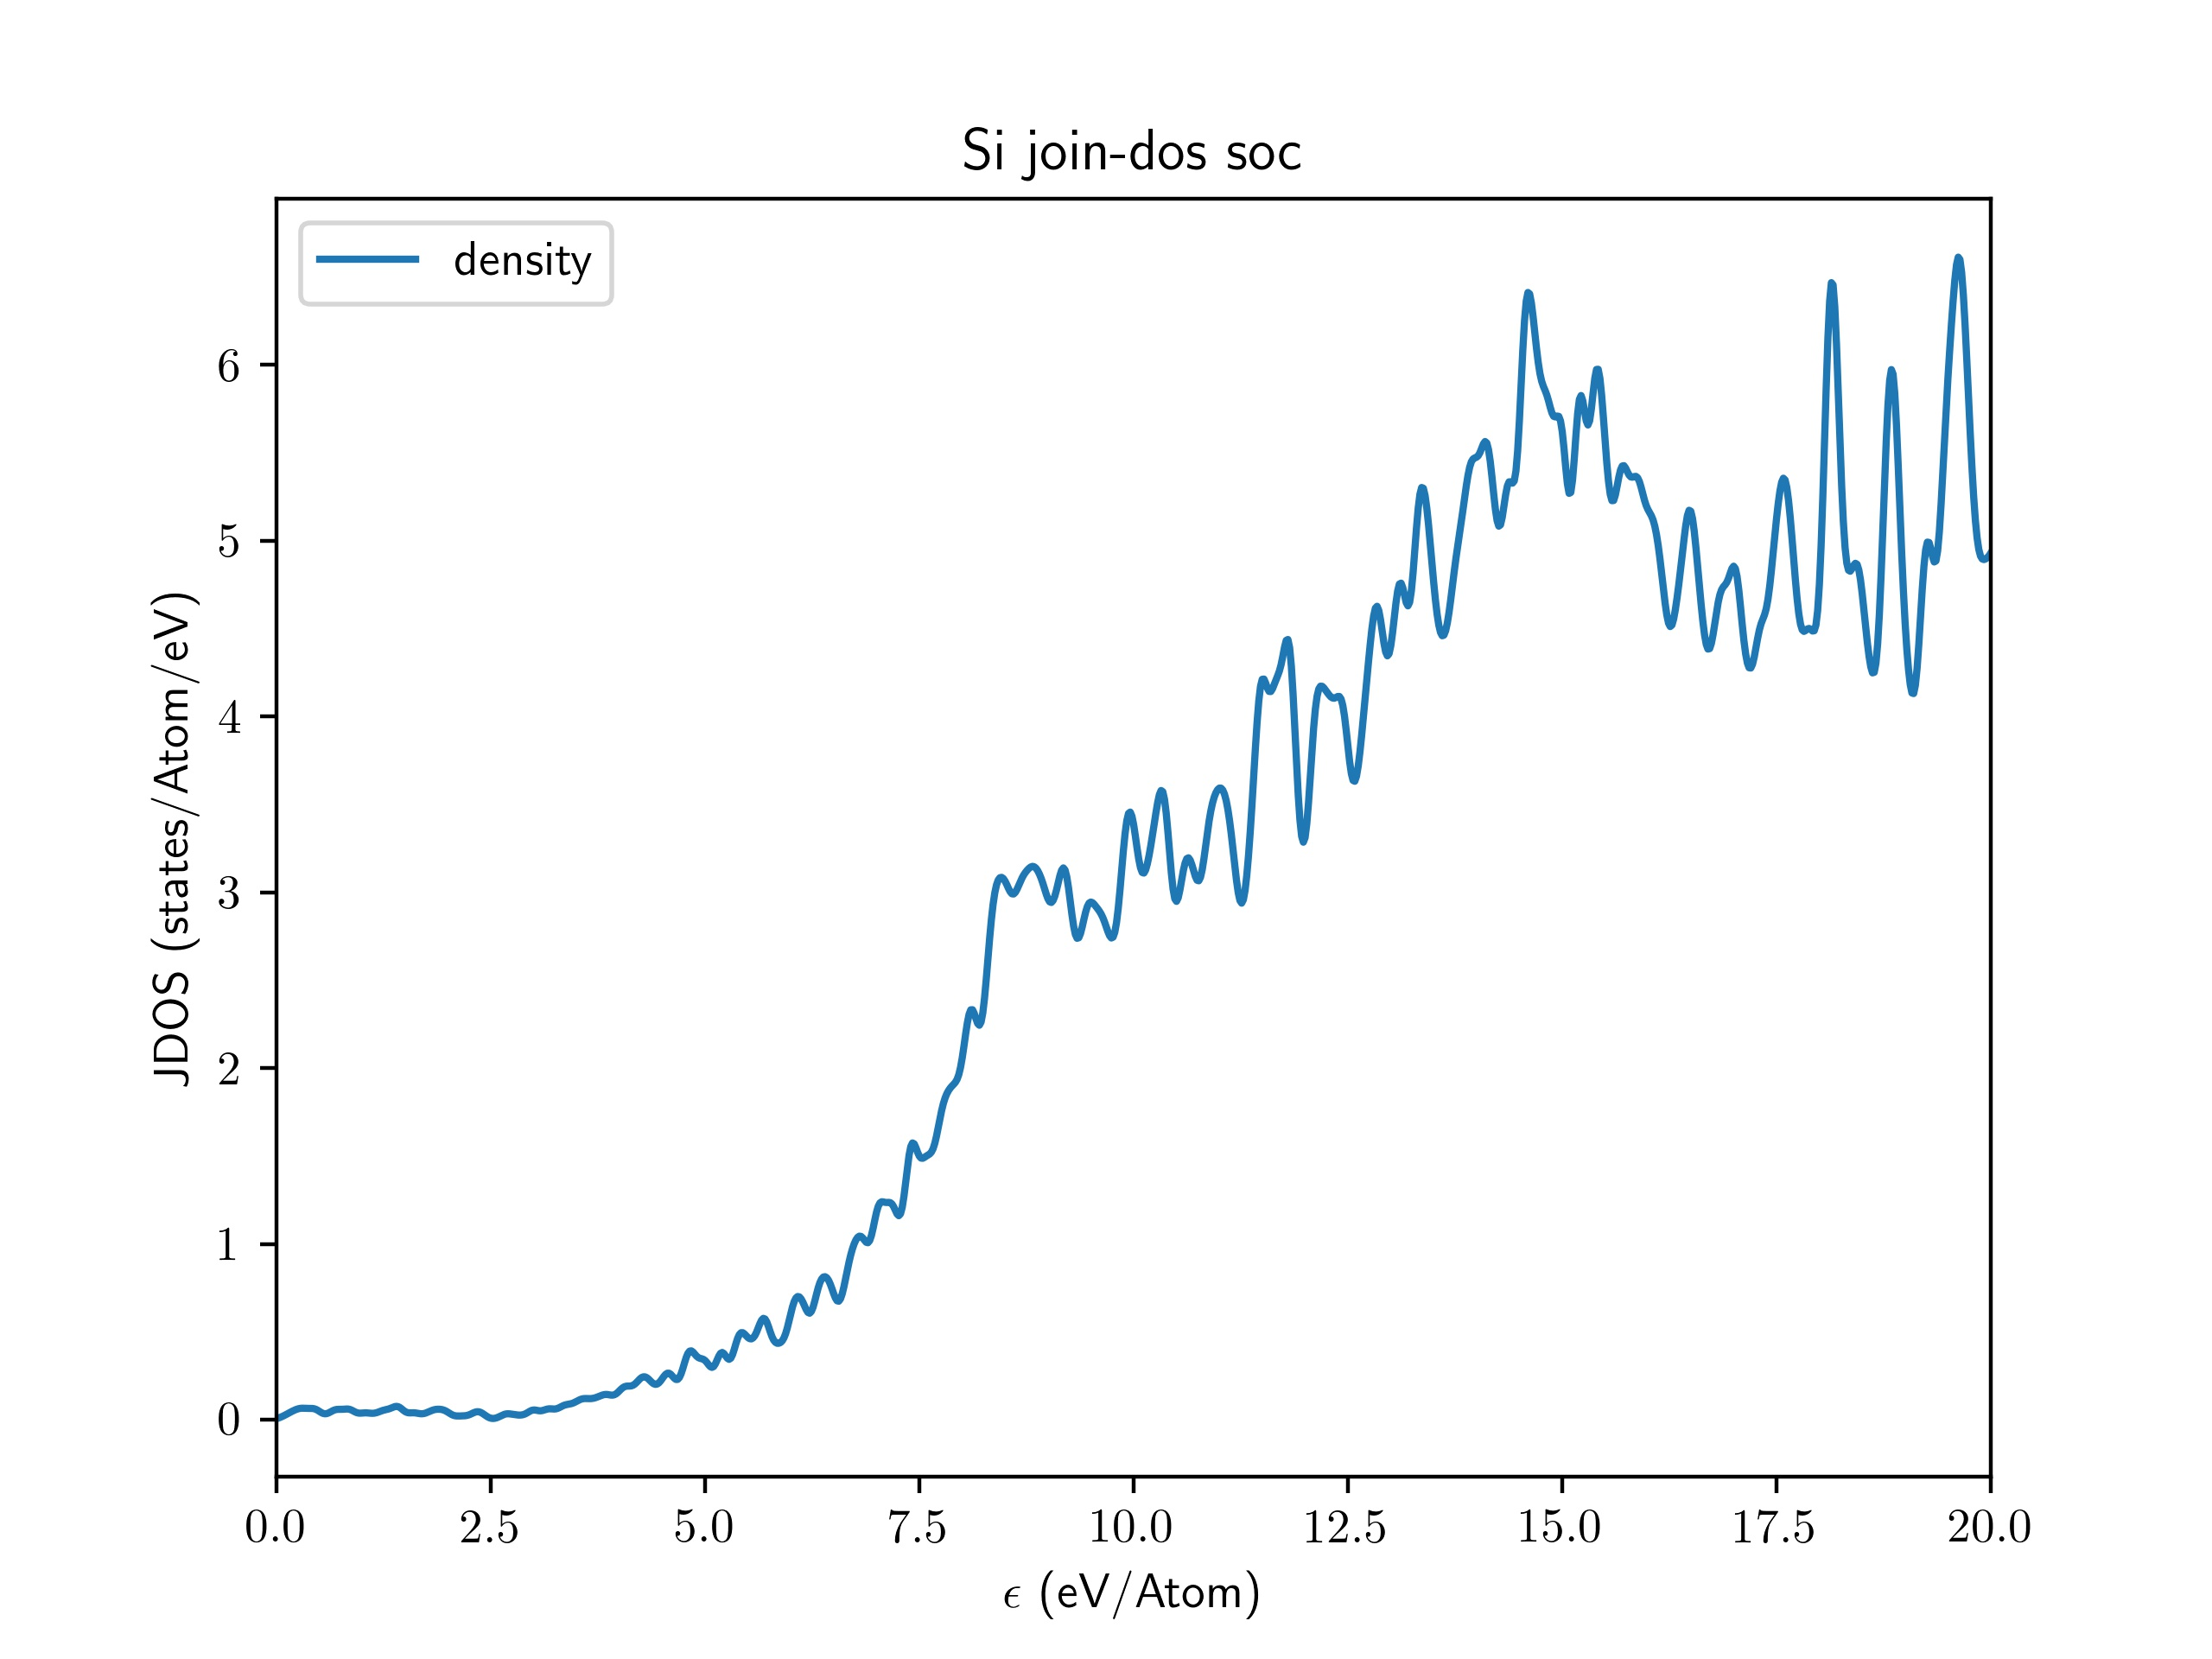
\includegraphics[width=\textwidth]{{data/q2/All_Data/Si_data/Si_soc_jdos}.jpg}
					\caption{Si join-DOS with SOC}
					\label{fig:Sisocjdos}
				\end{minipage}
				\begin{minipage}[b]{0.45\textwidth}
					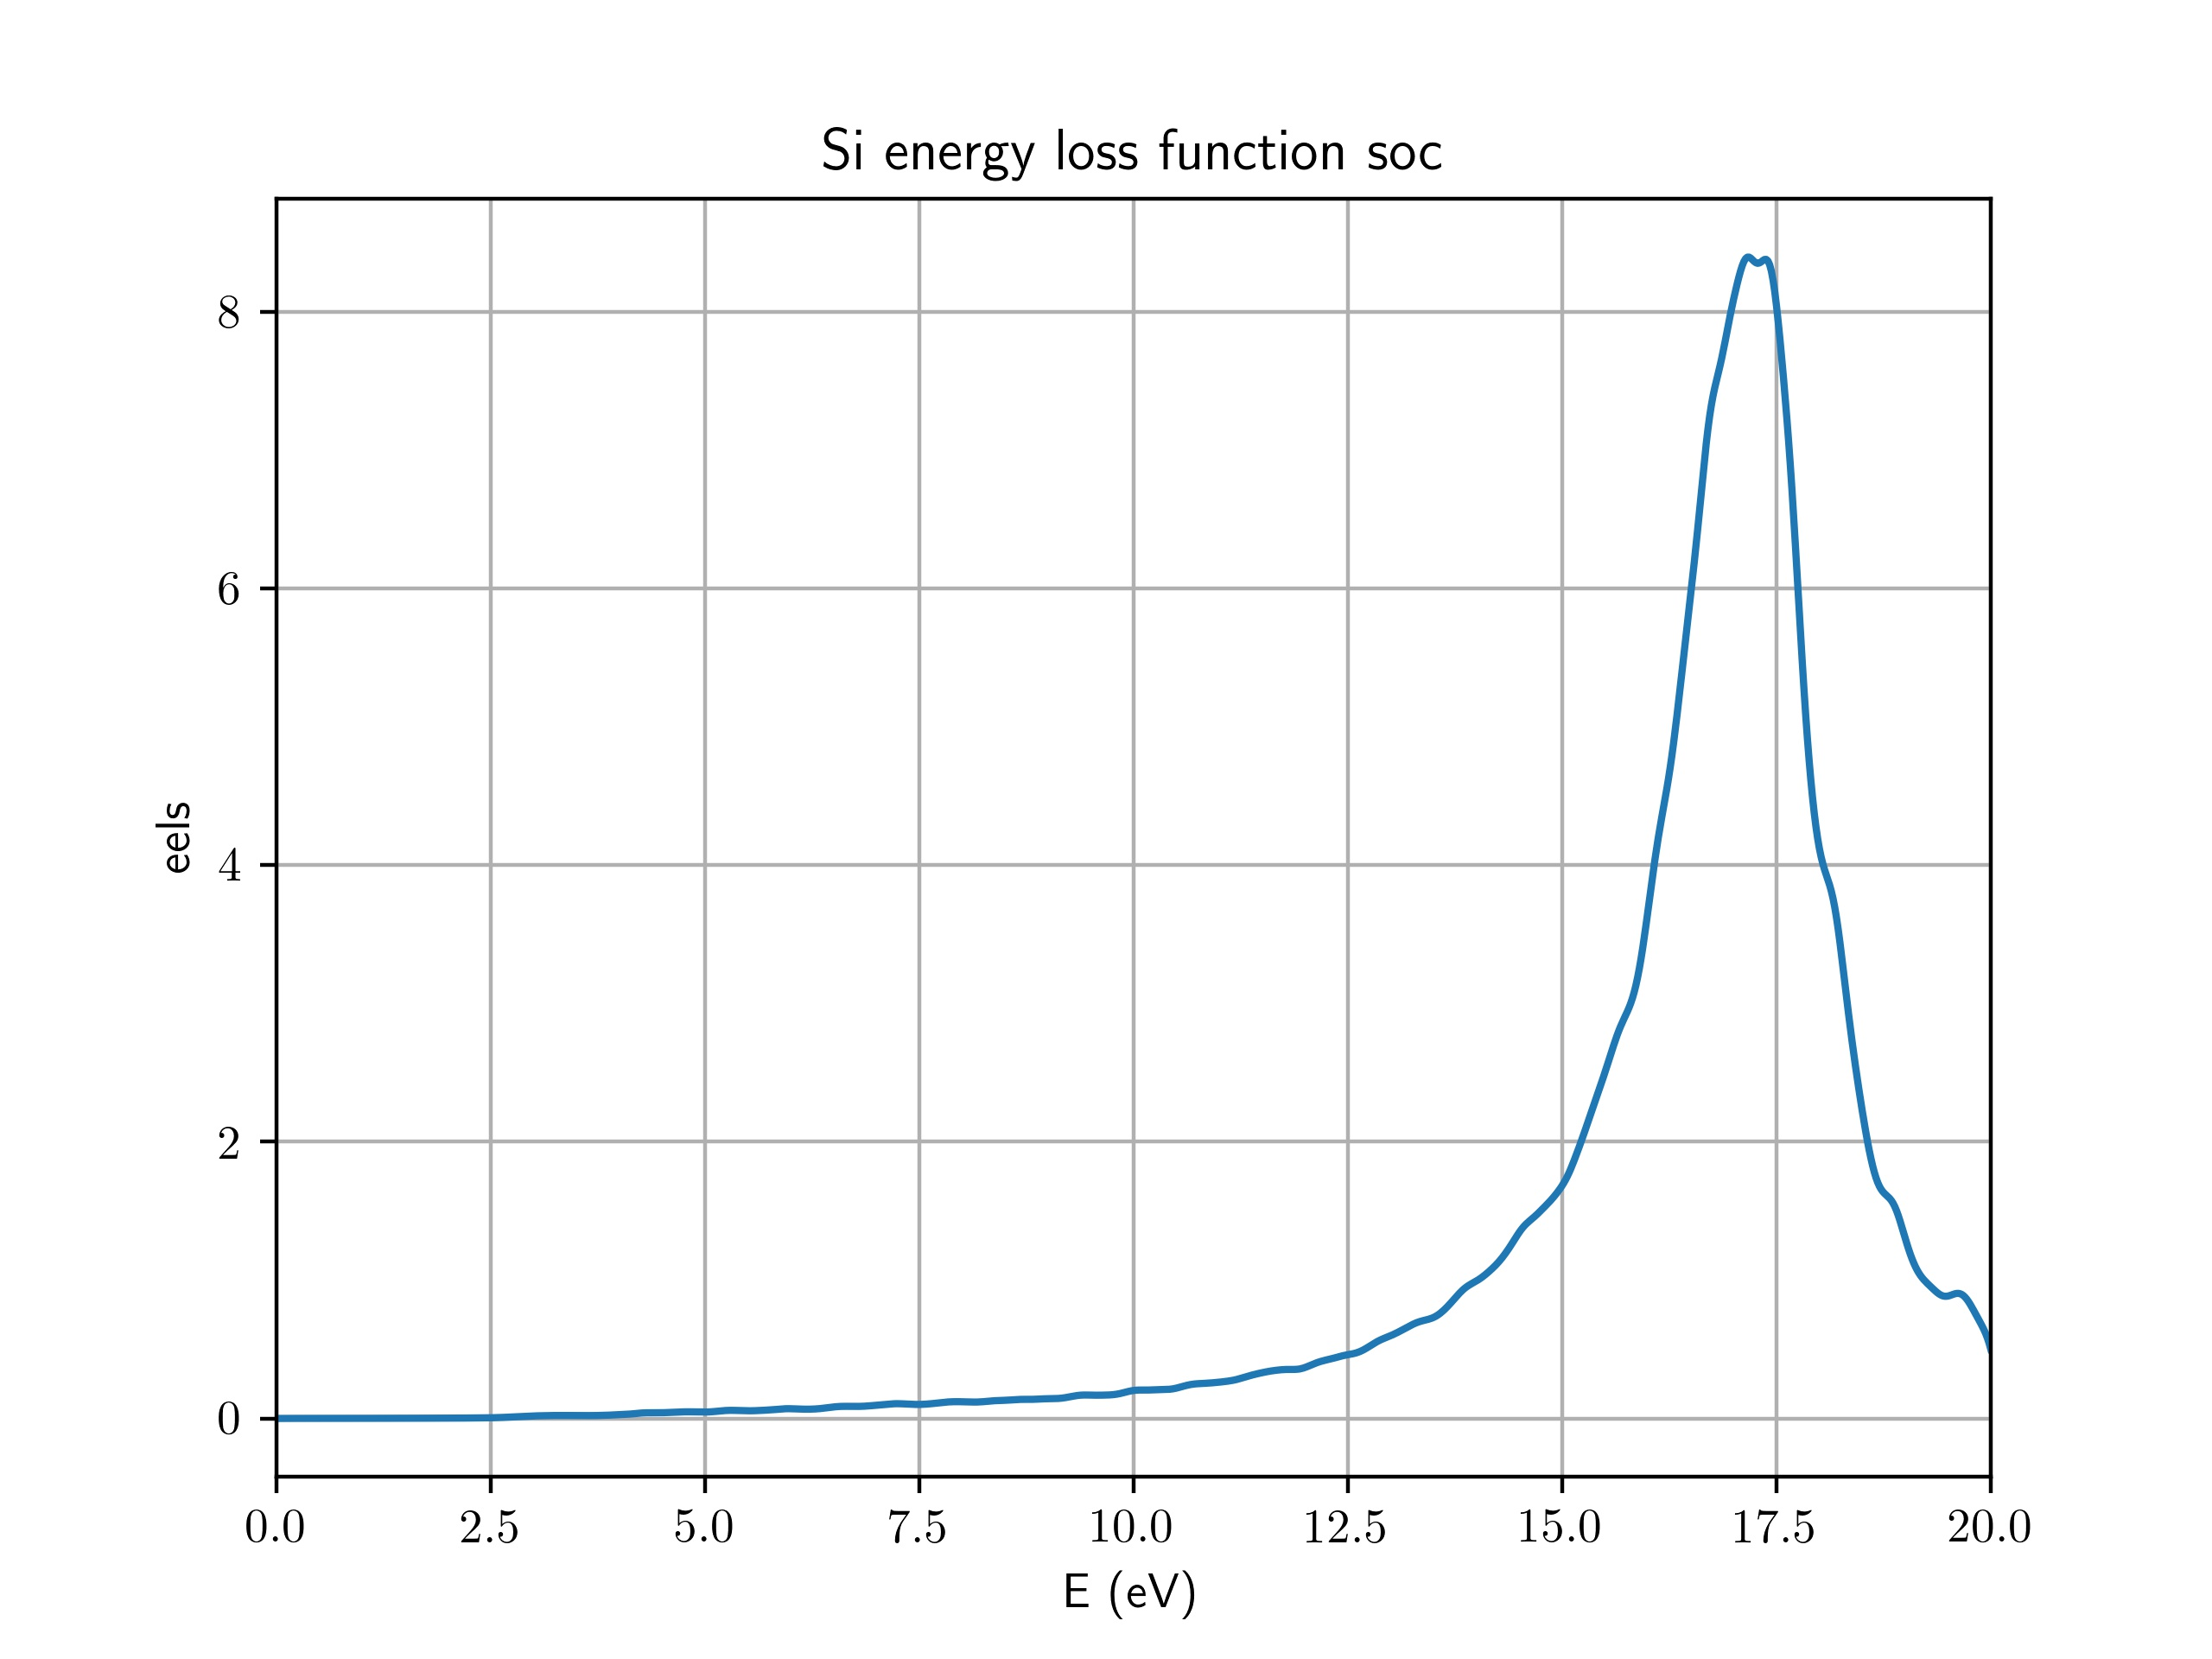
\includegraphics[width=\textwidth]{{data/q2/All_Data/Si_data/Si_soc_eels}.jpg}
					\caption{Si energy loss function with SOC}
					\label{fig:Sisoceels}
				\end{minipage}
				
			\end{figure} 
			\begin{figure}[h!]
				\begin{minipage}[b]{0.45\textwidth}
					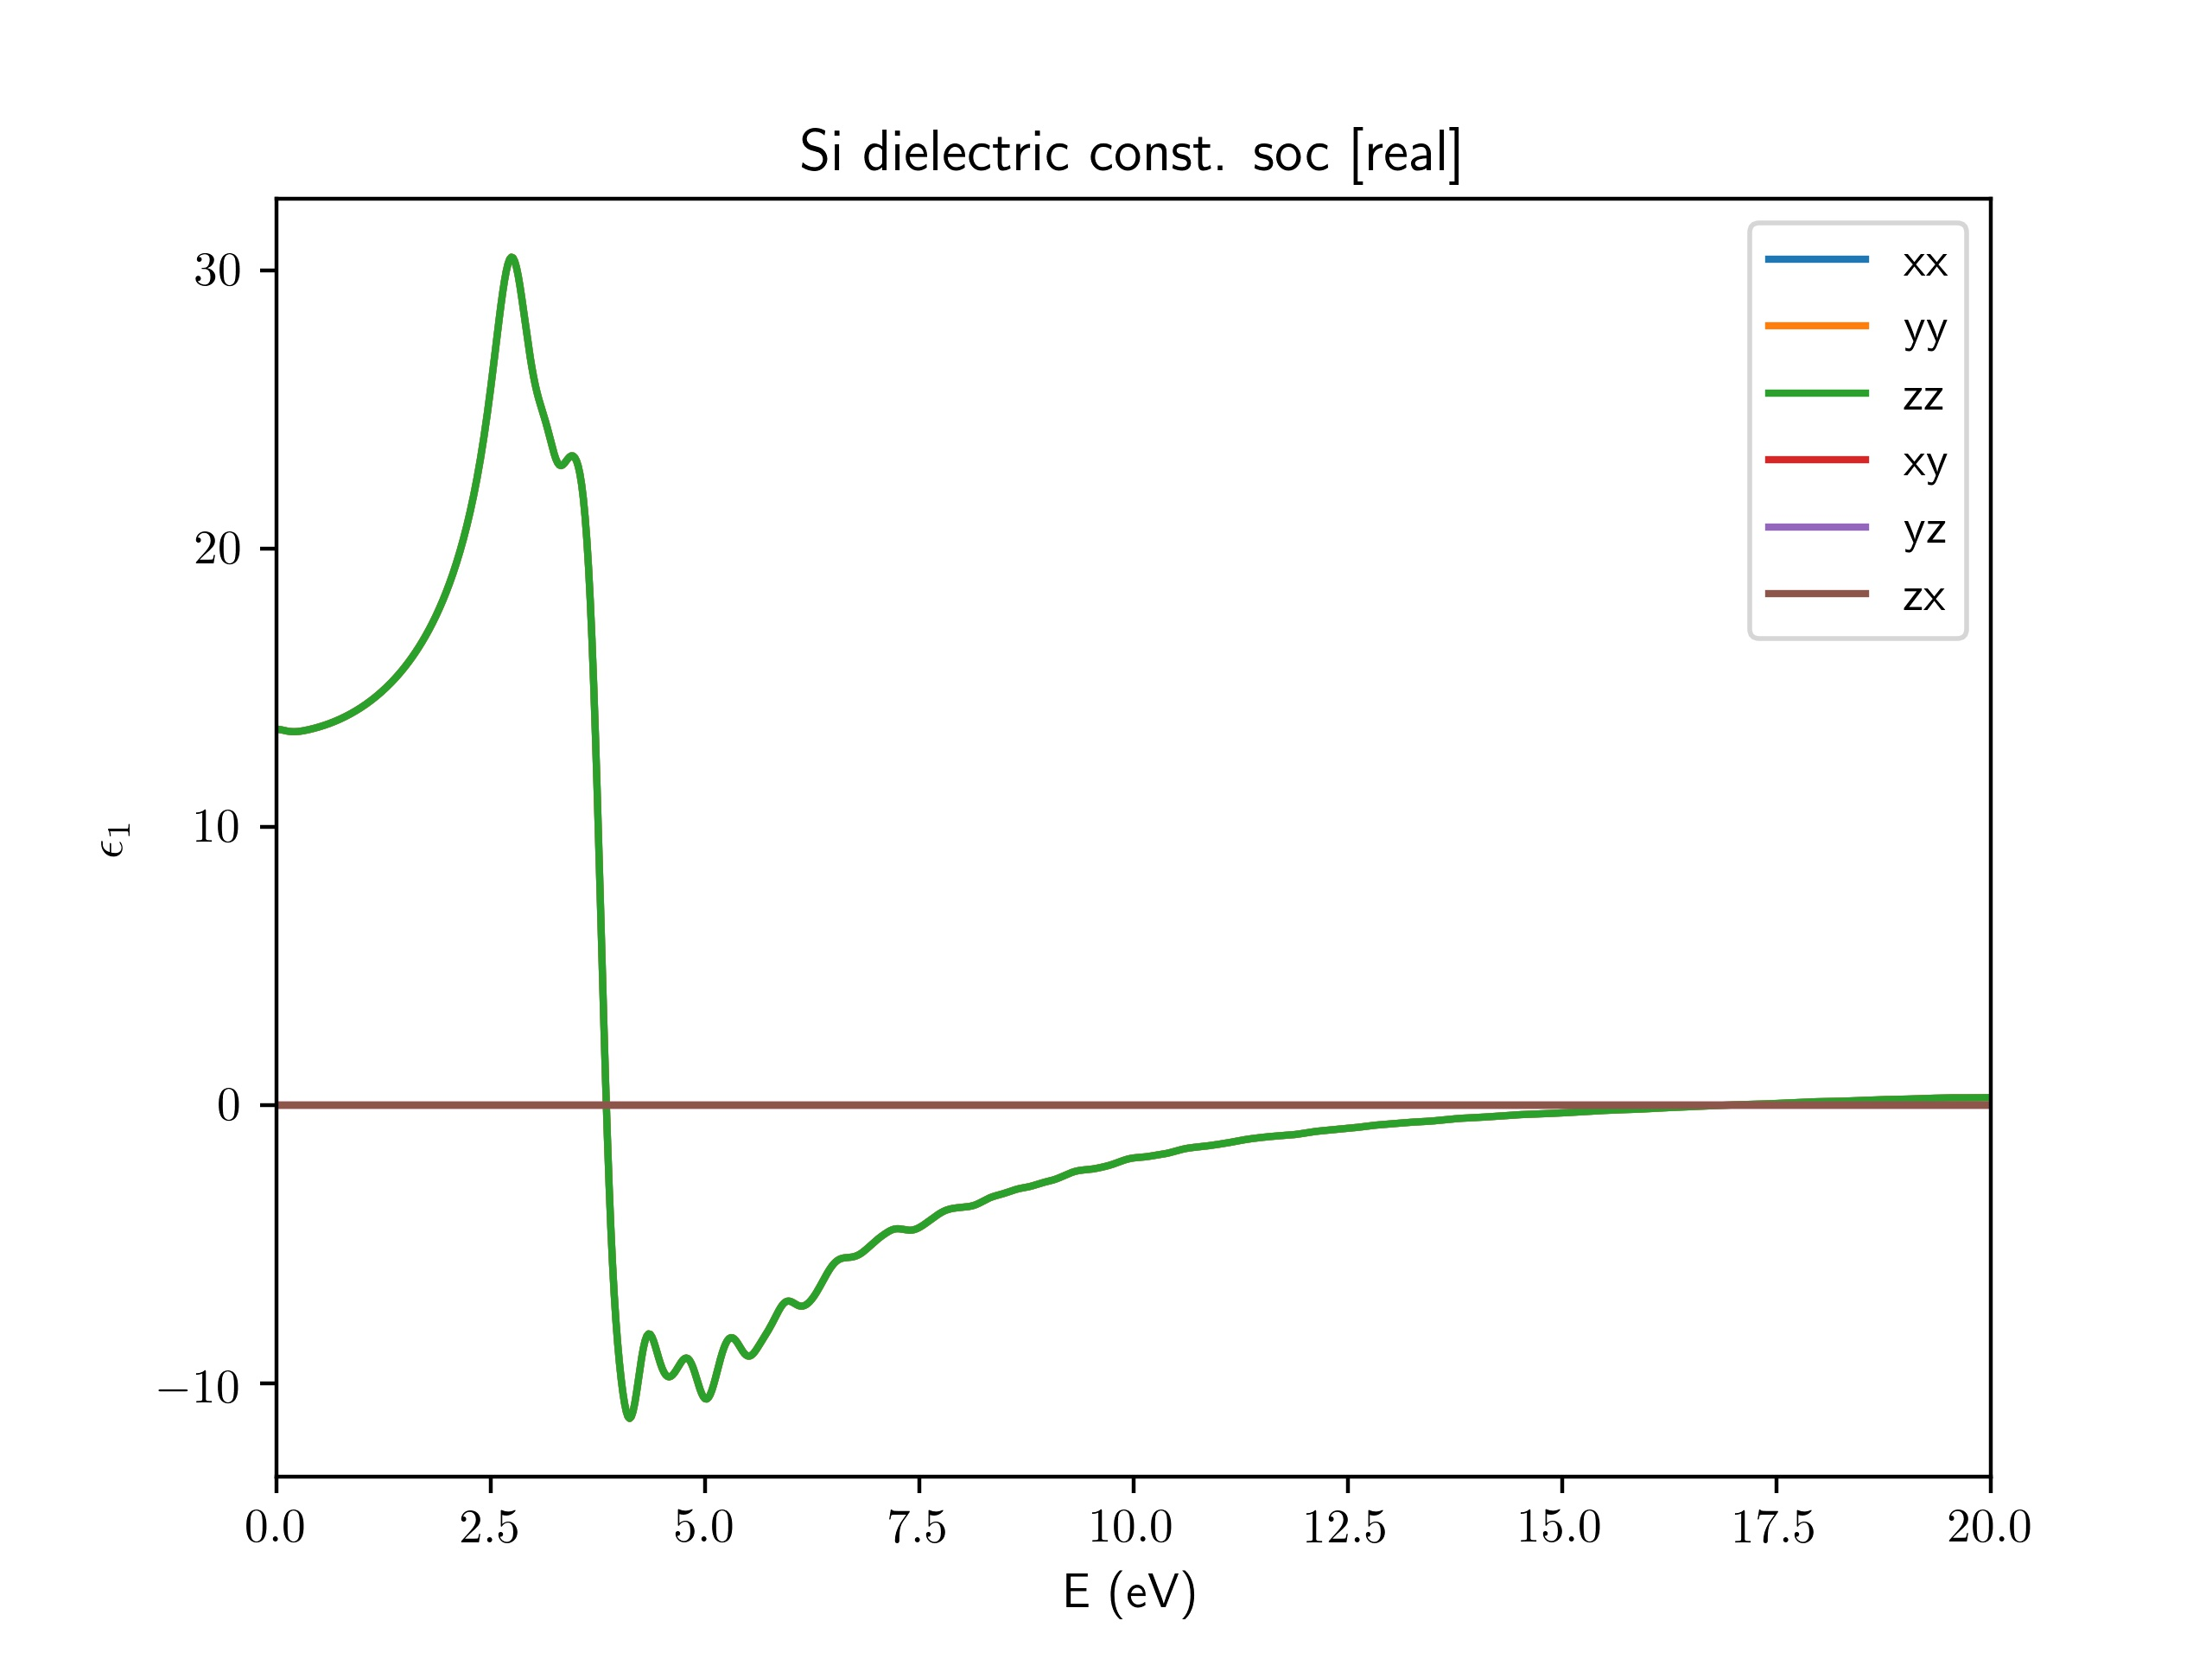
\includegraphics[width=\textwidth]{{data/q2/All_Data/Si_data/Si_soc_epsre}.jpg}
					\caption{Si dielectric constant (real) with SOC}
					\label{fig:Sisocepsre}
				\end{minipage}
				\begin{minipage}[b]{0.45\textwidth}
					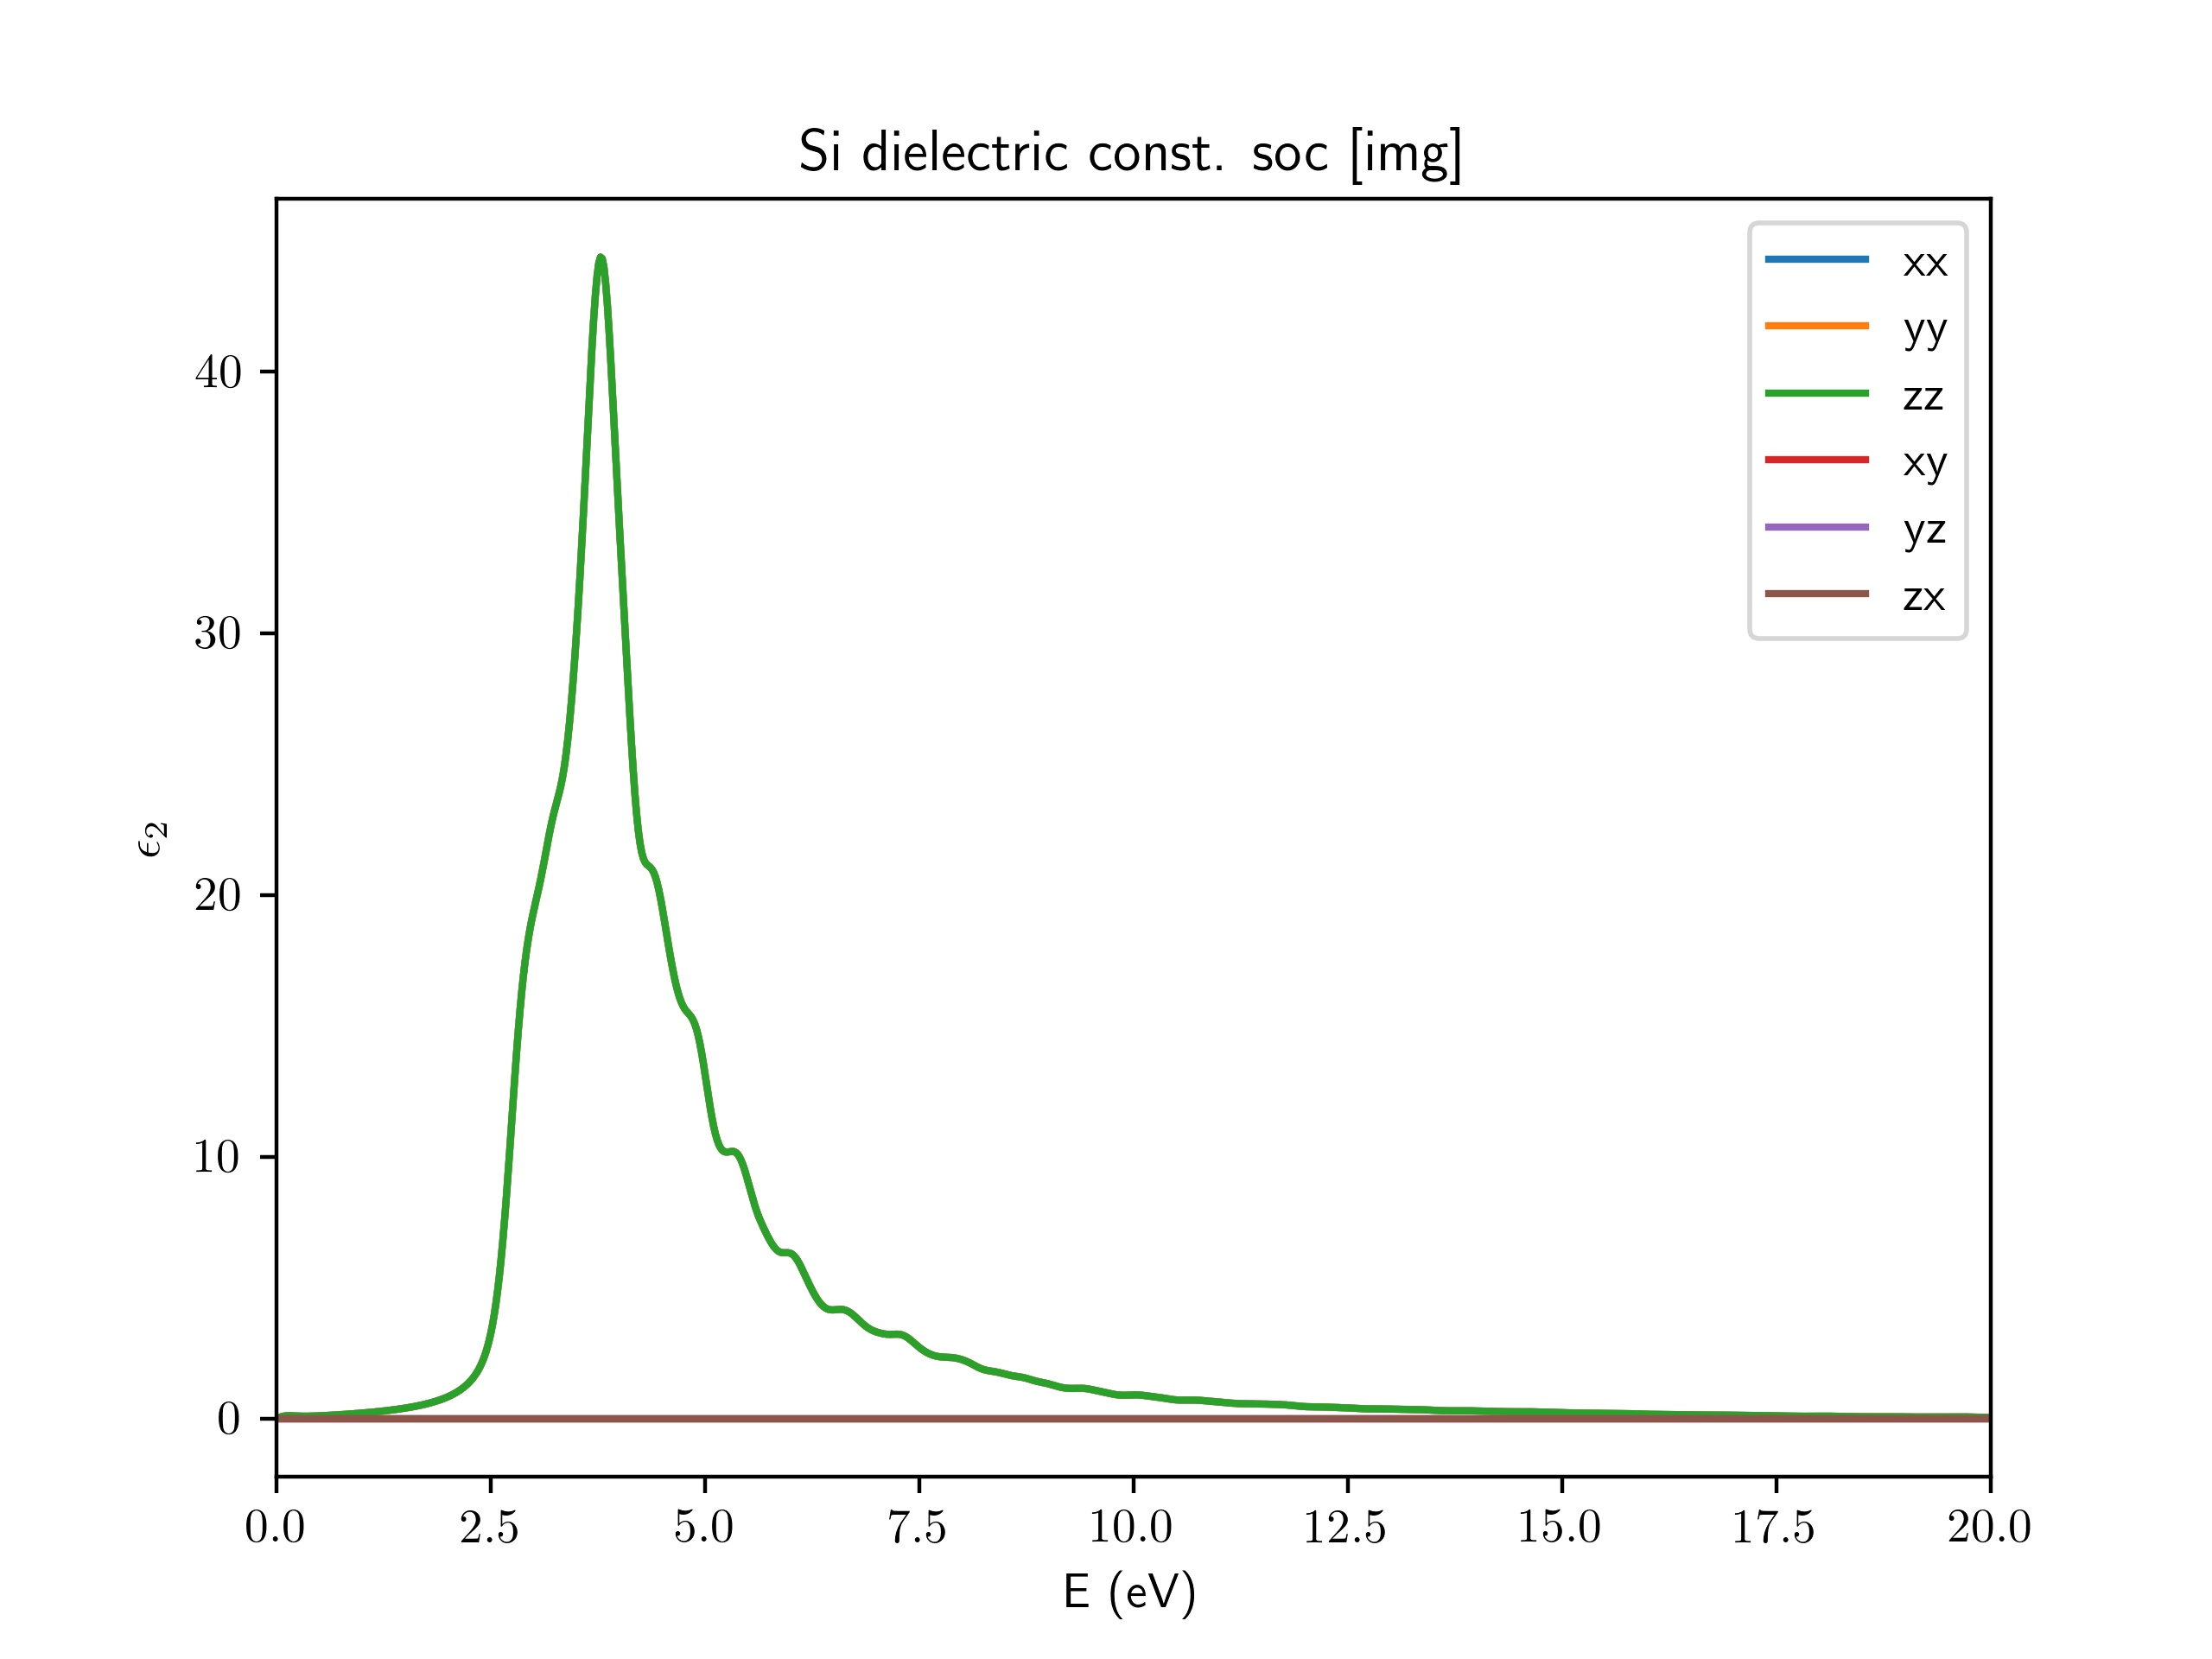
\includegraphics[width=\textwidth]{{data/q2/All_Data/Si_data/Si_soc_epsim}.jpg}
					\caption{Si dielectric constant (image) with SOC}
					\label{fig:Sisocepsim}
				\end{minipage}
				\begin{minipage}[b]{0.45\textwidth}
					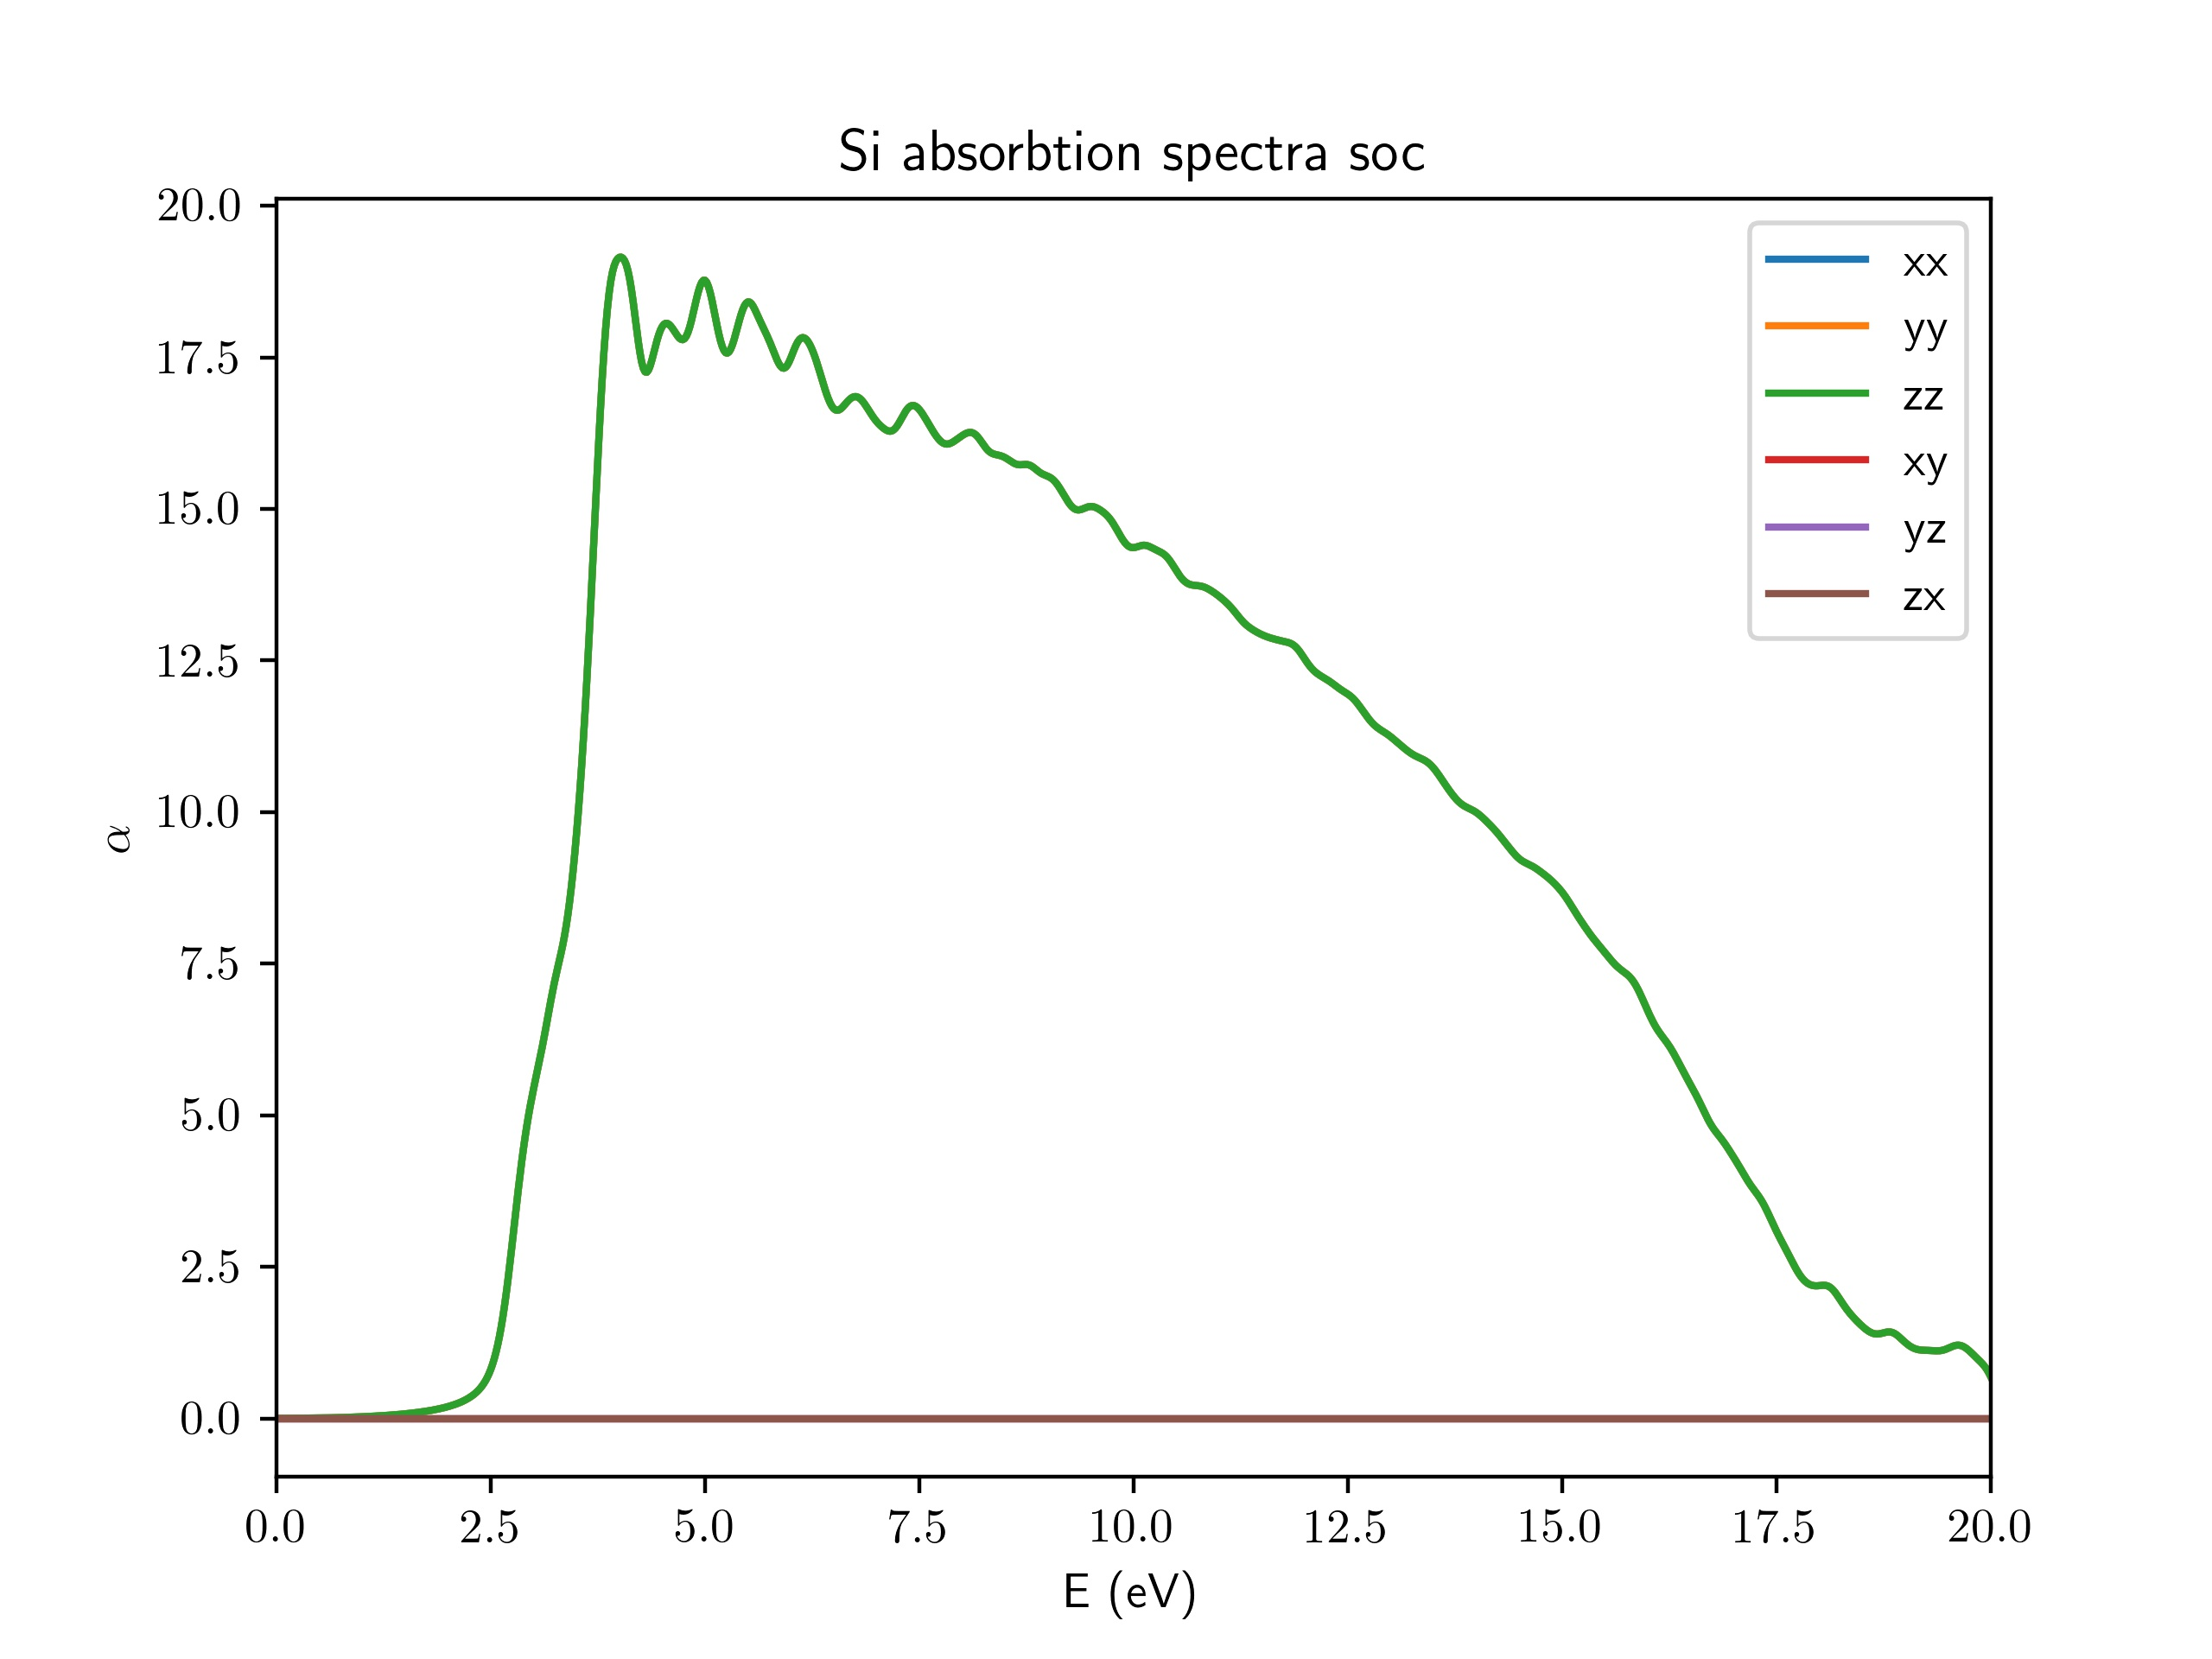
\includegraphics[width=\textwidth]{{data/q2/All_Data/Si_data/Si_soc_alpha}.jpg}
					\caption{Si absorption with SOC}
					\label{fig:Sisocalpha}
				\end{minipage}
			\end{figure} 
		\end{itemize}
		
	\end{enumerate}
	\clearpage

	%q3:
	\item GGA-PBE calculation of Si and it's thermal dynamic properties.
	
	\begin{enumerate}[label=(\alph*)]
		\item Using GGA-PBE potential with structure optimization, the relaxed lattice constant is calculated as :
		\begin{equation}
			a_0  = 5.3945 \AA
		\end{equation}
		
		By self-consistent calculation, the band structure is calculated. Show as following:
		\begin{figure}[h!]
			\begin{minipage}[b]{0.5\textwidth}
				\includegraphics[width=\textwidth]{{data/q3/Si}.jpg}
				\caption{Si band-structure calculated with GGA-PBE potential}
				\label{fig:Sipbeband}
			\end{minipage}
		\end{figure} 
		
		The calculated band structure consist with previous work \cite{LIU20151384}.
		
		\item For phonon dispersion. The following results are calculated with the relaxed lattice constant with 2x2x2 super cell and 3x3x3 super cell respectively.
		\begin{figure}[h!]
			\begin{minipage}[b]{0.5\textwidth}
				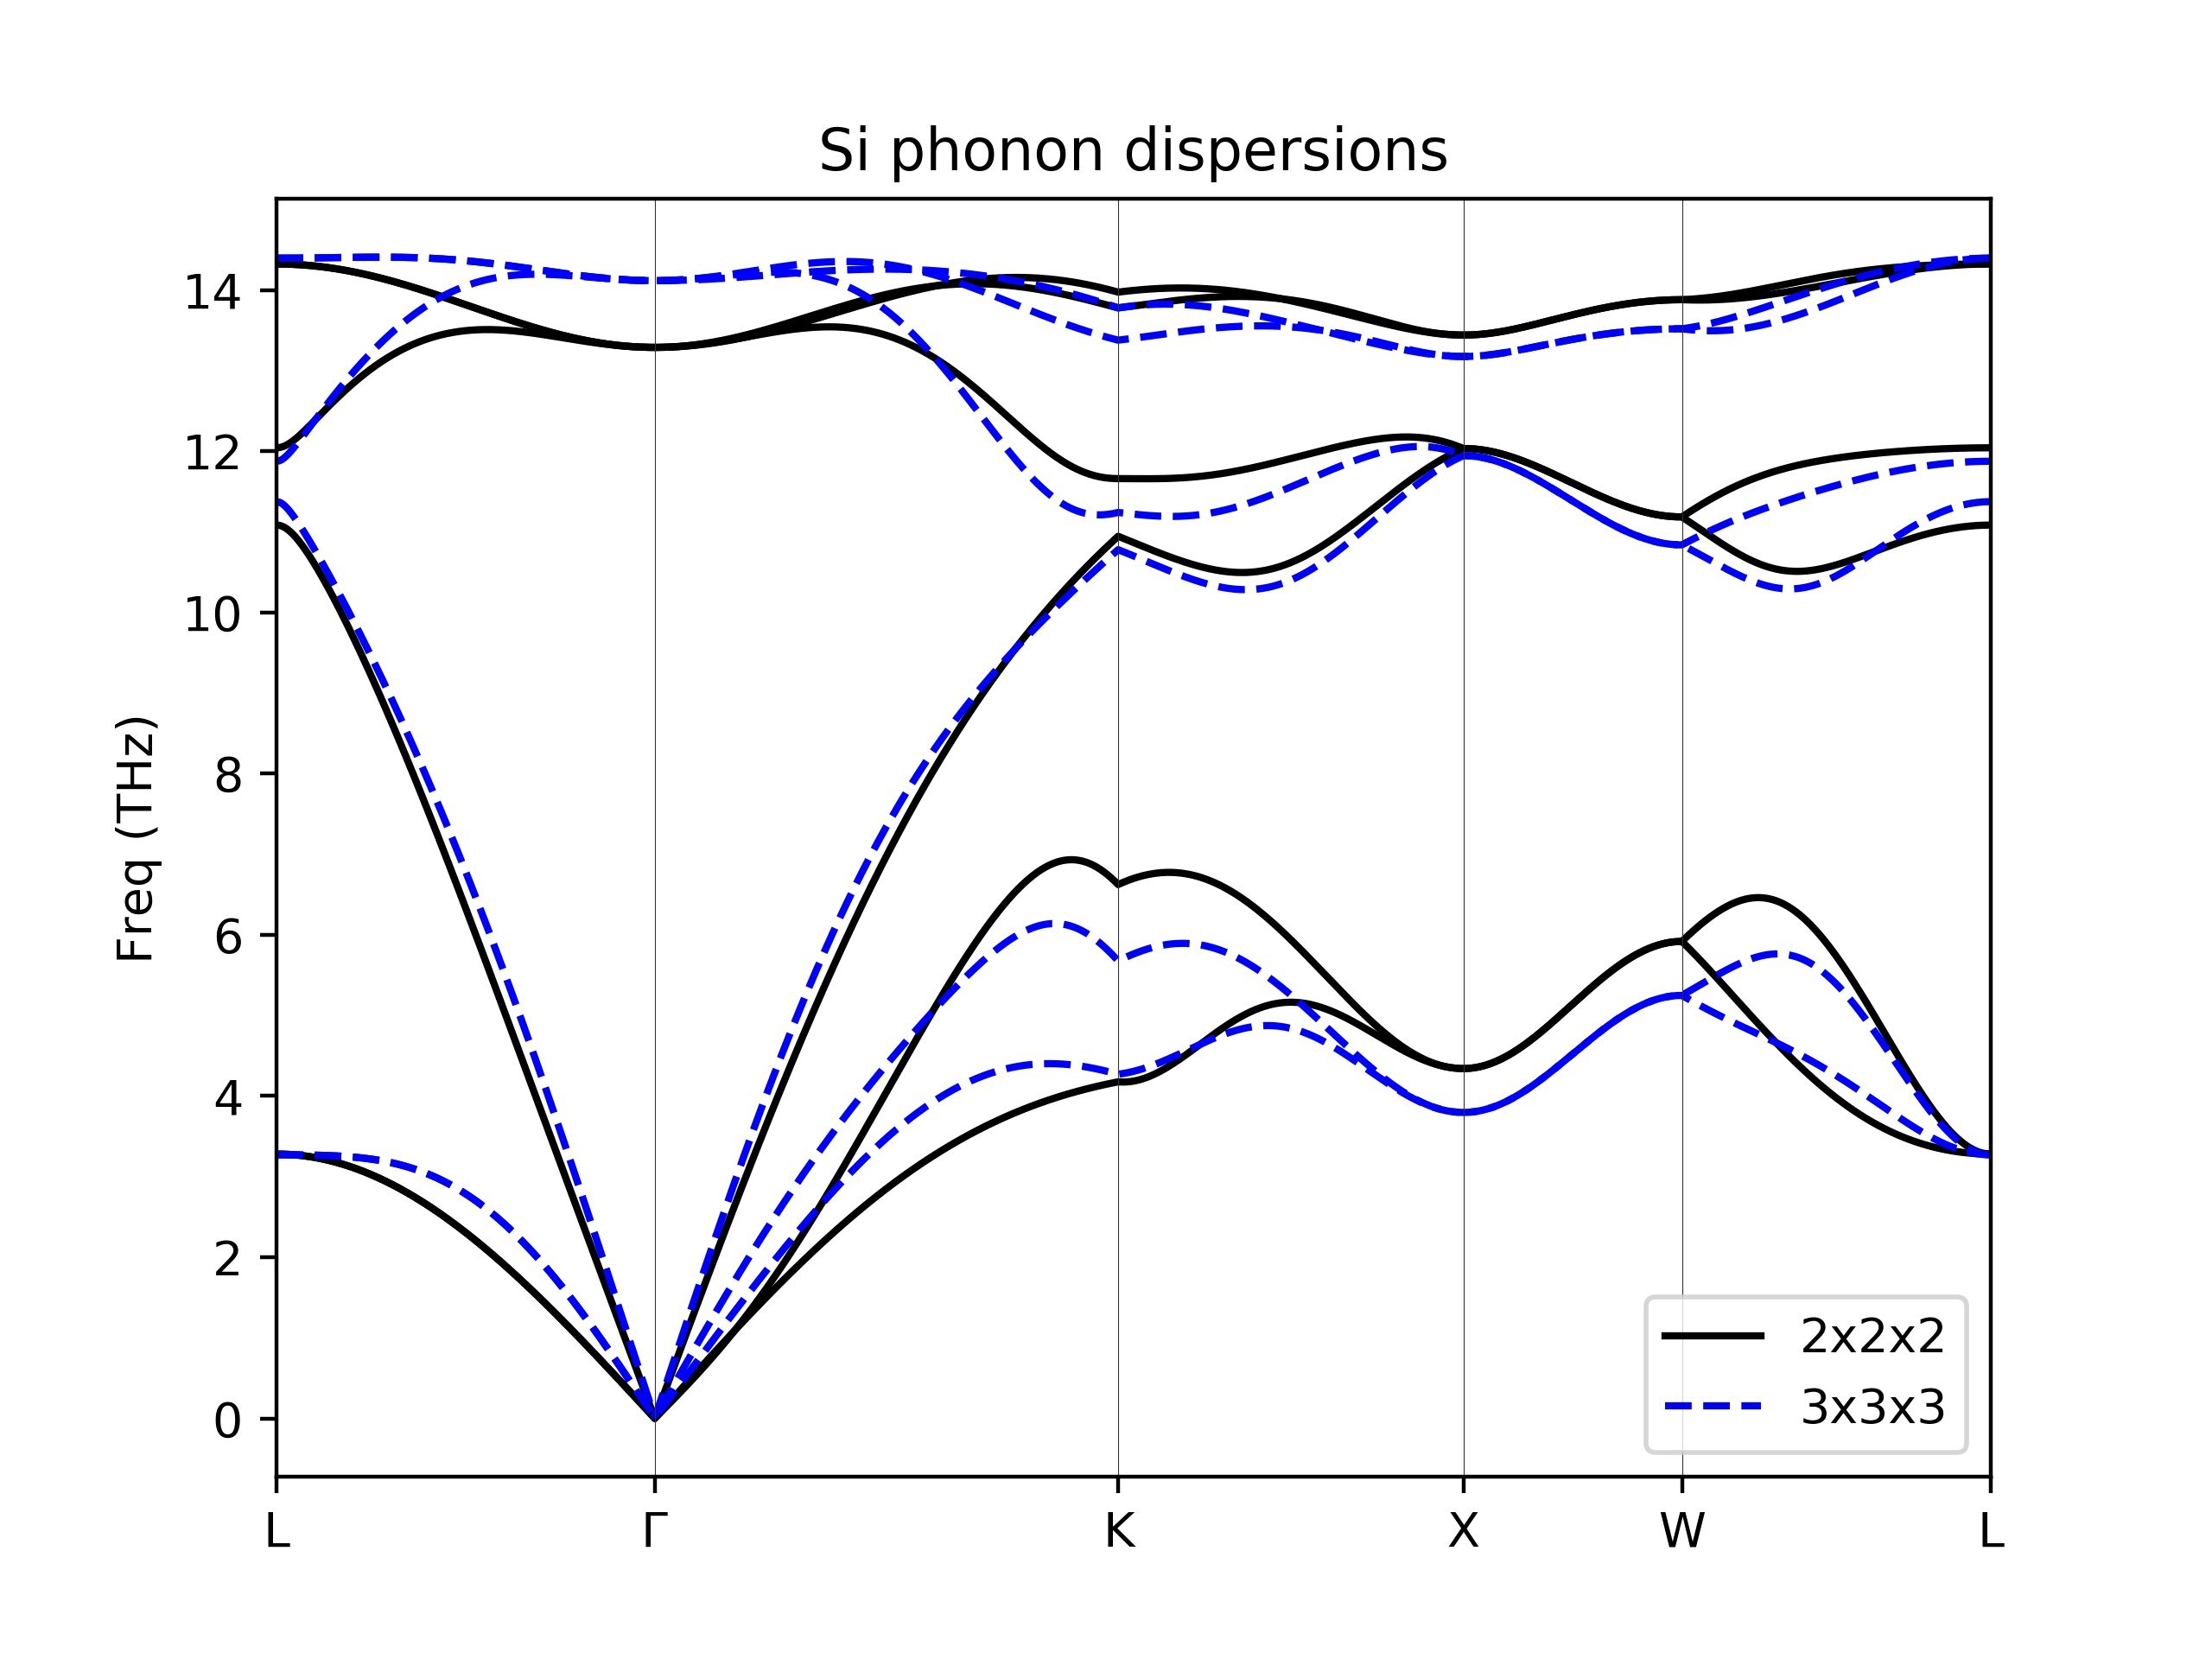
\includegraphics[width=\textwidth]{{data/q3/Si_dispr}.jpg}
				\caption{Si phonon dispersion calculated with GGA-PBE potential}
				\label{fig:Sipbedispr}
			\end{minipage}
		\end{figure} 		
	
		\item Following shows the thermal dynamic properties of internal energy, free energy, entropy and specific heat results with 2x2x2 super cell and 3x3x3 super cell respectively.
		\begin{figure}[h!]
			\begin{minipage}[b]{0.45\textwidth}
				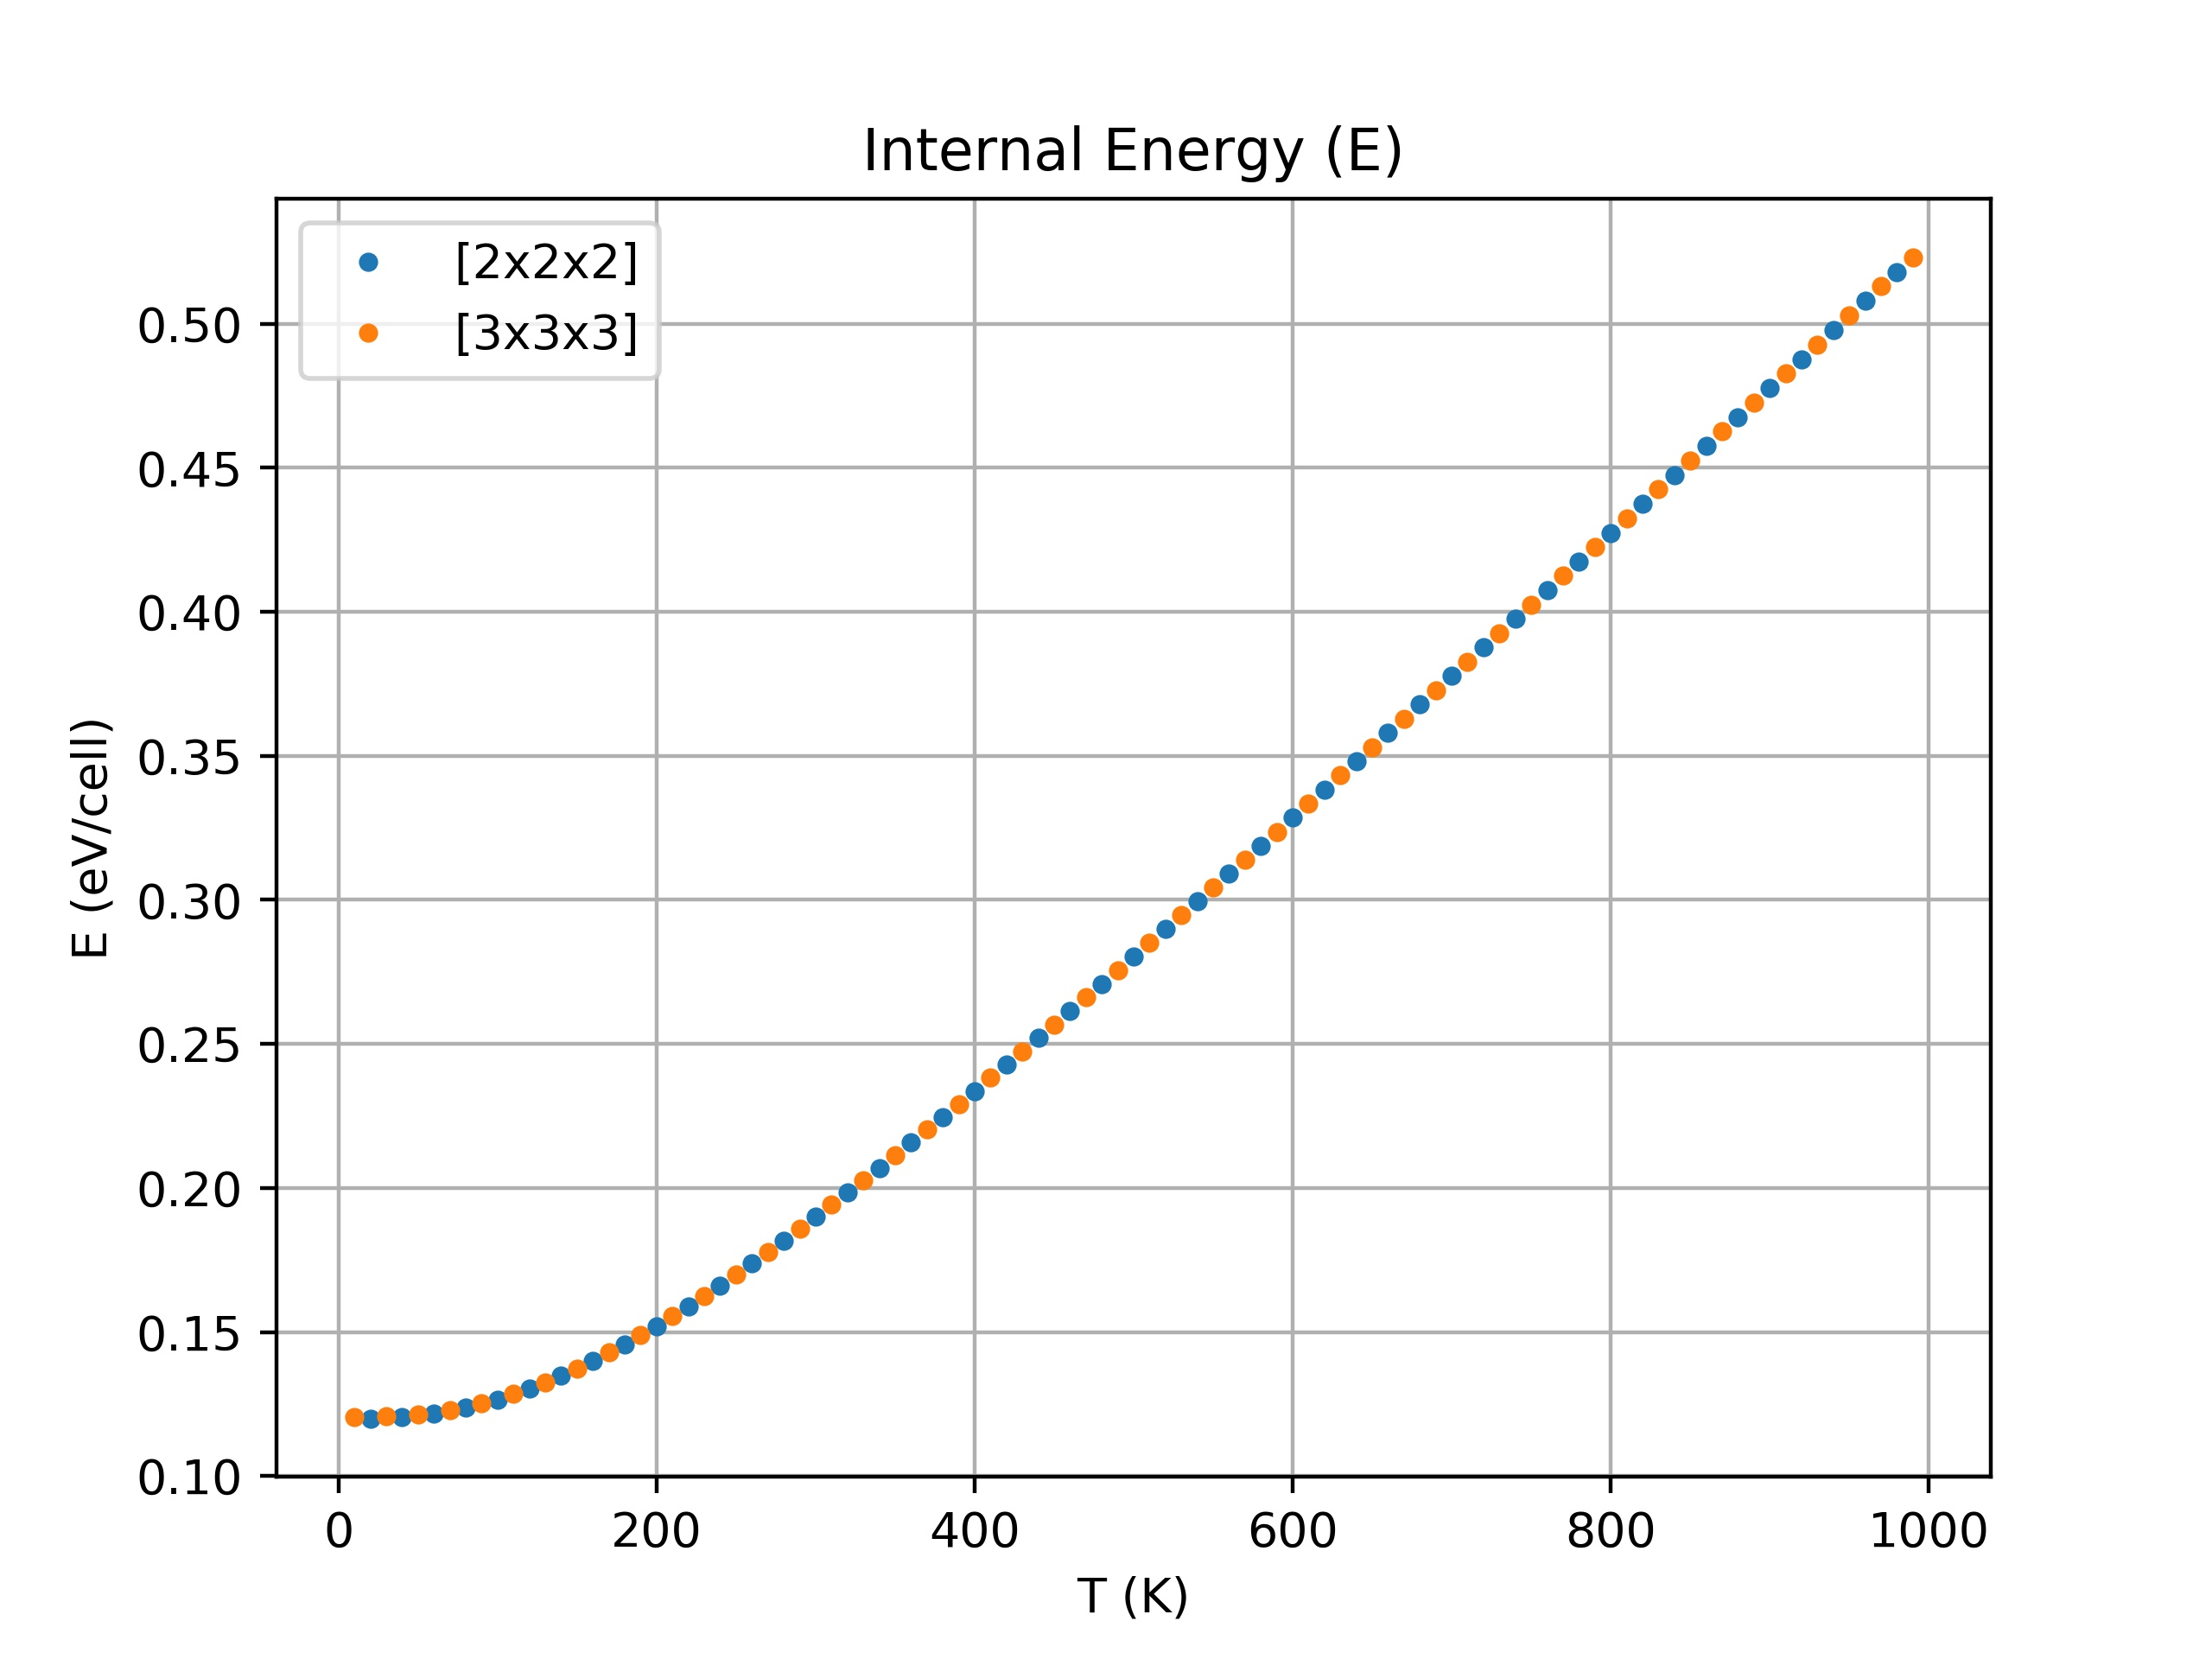
\includegraphics[width=\textwidth]{{data/q3/Si_E}.jpg}
				\caption{Si internal energy}
				\label{fig:SiE}
			\end{minipage}
			\begin{minipage}[b]{0.45\textwidth}
				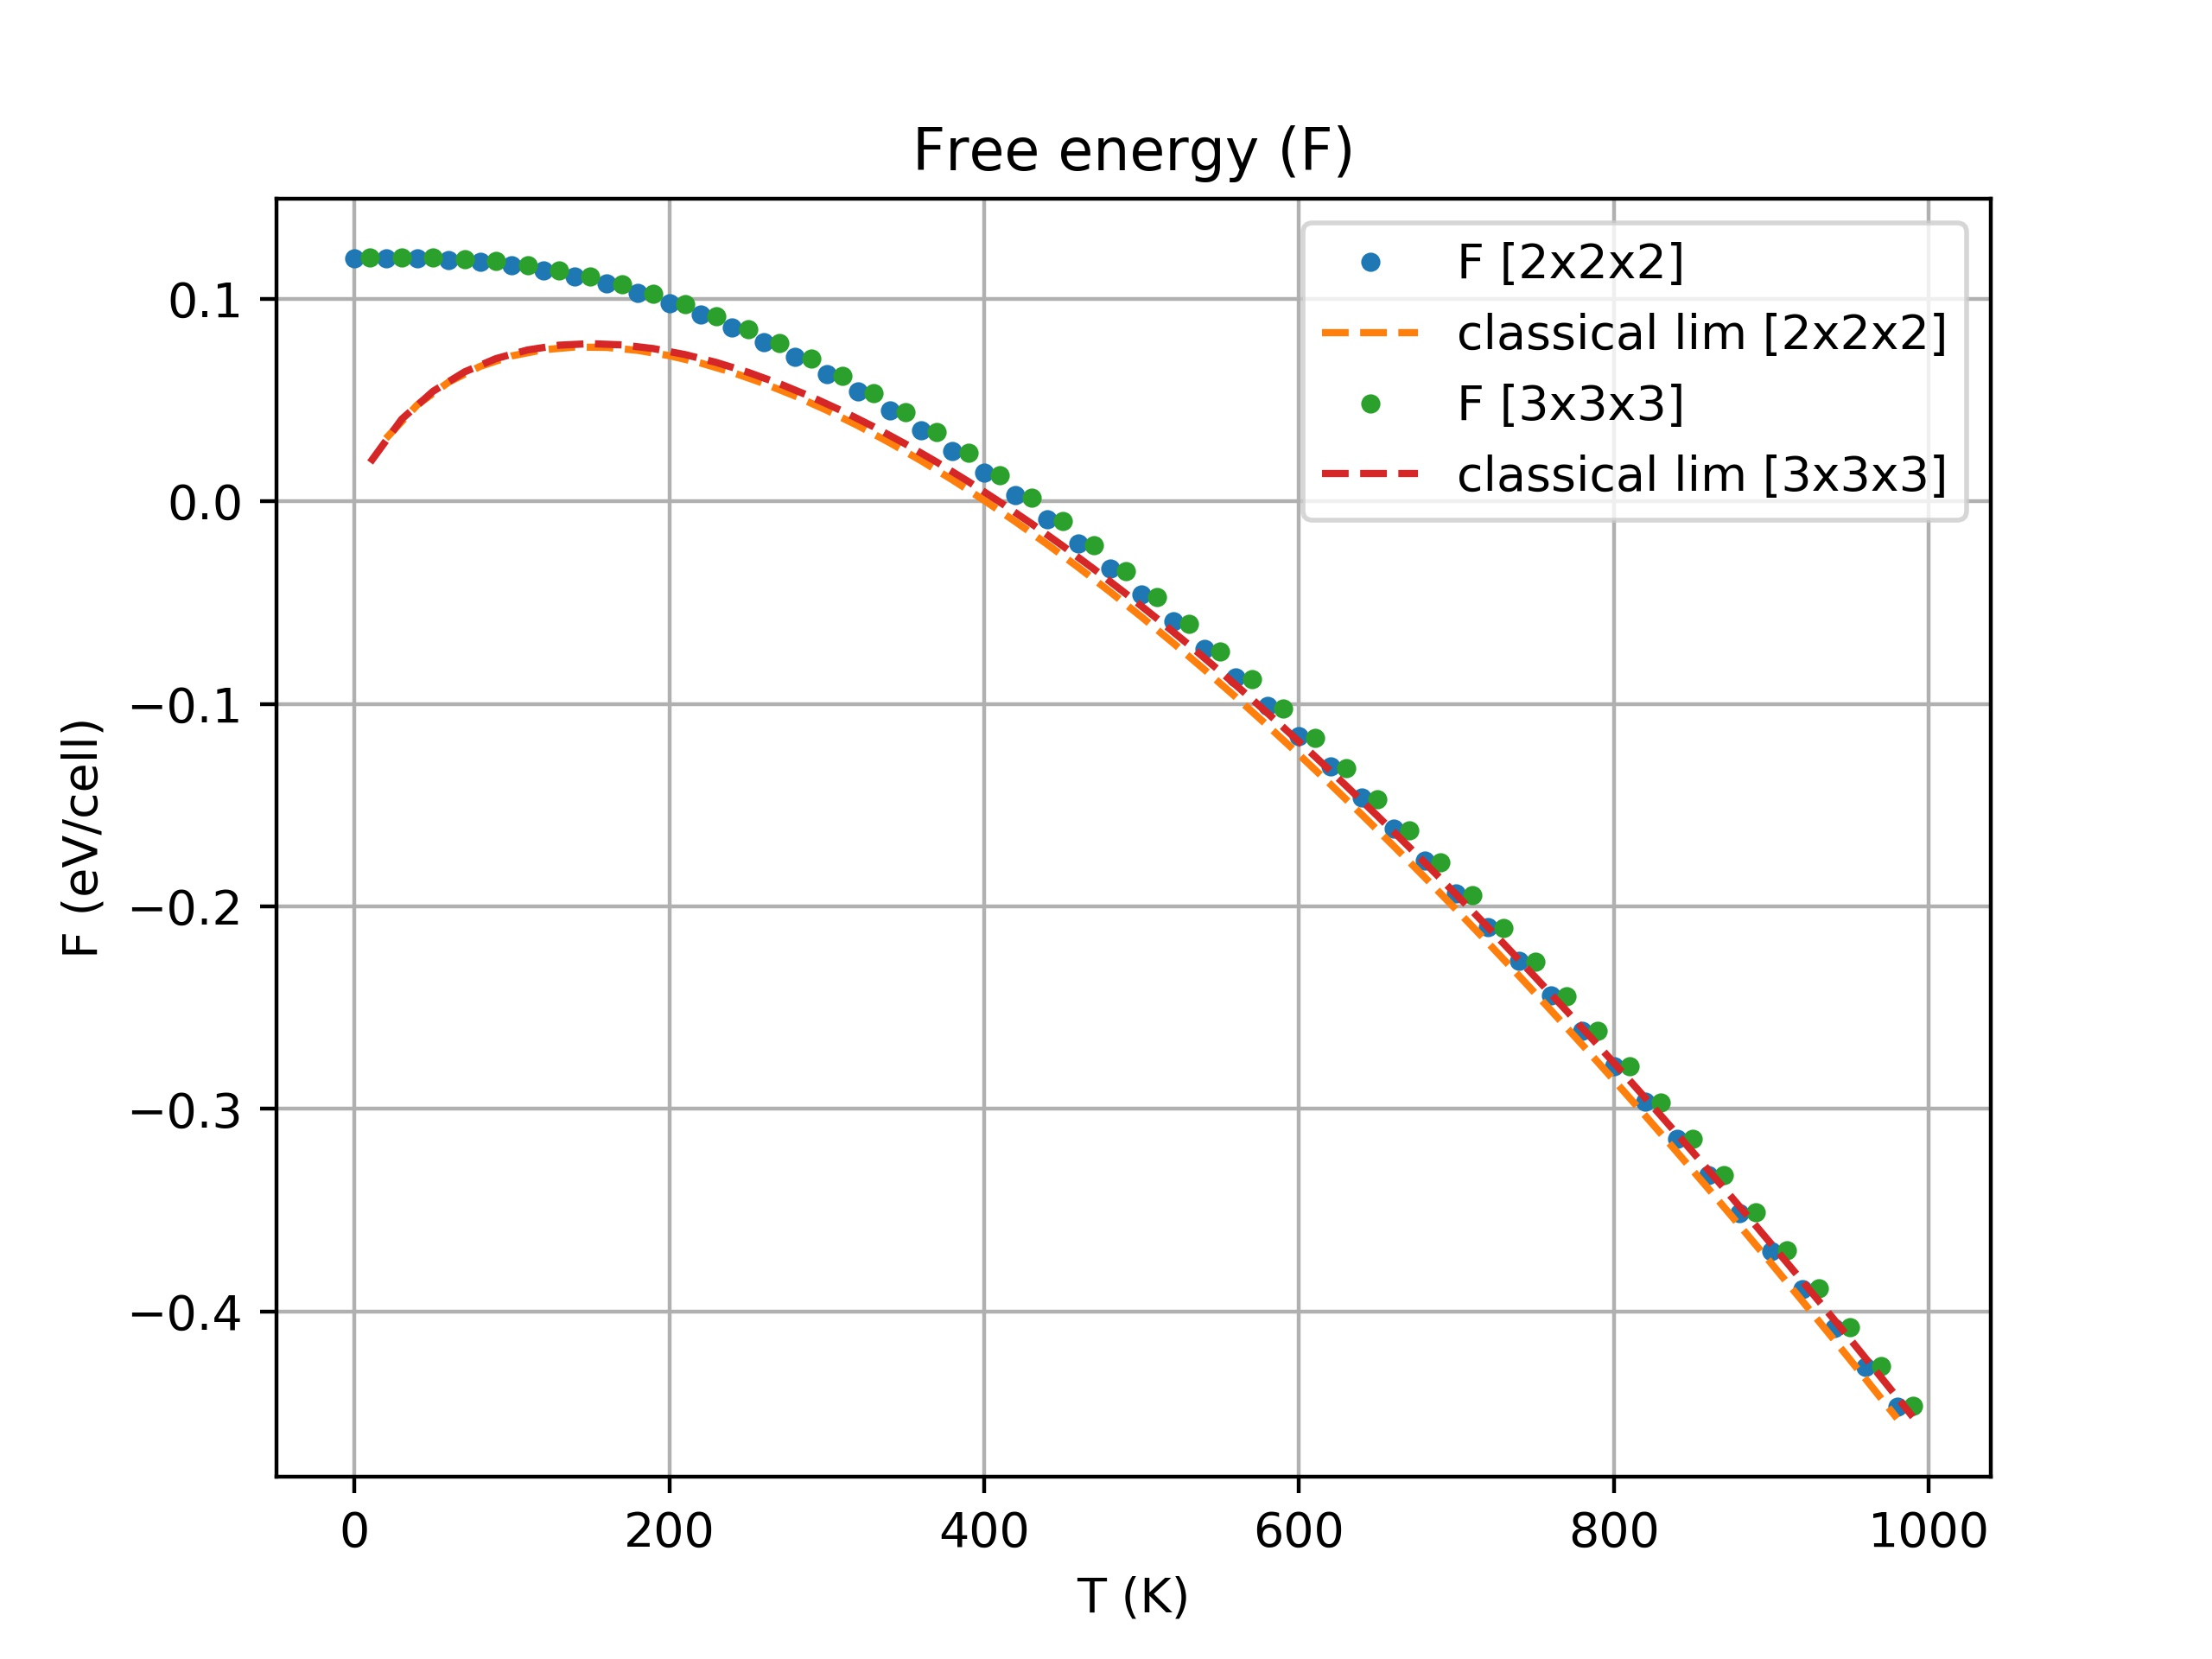
\includegraphics[width=\textwidth]{{data/q3/Si_F}.jpg}
				\caption{Si free energy}
				\label{fig:SiF}
			\end{minipage}
			\begin{minipage}[b]{0.45\textwidth}
				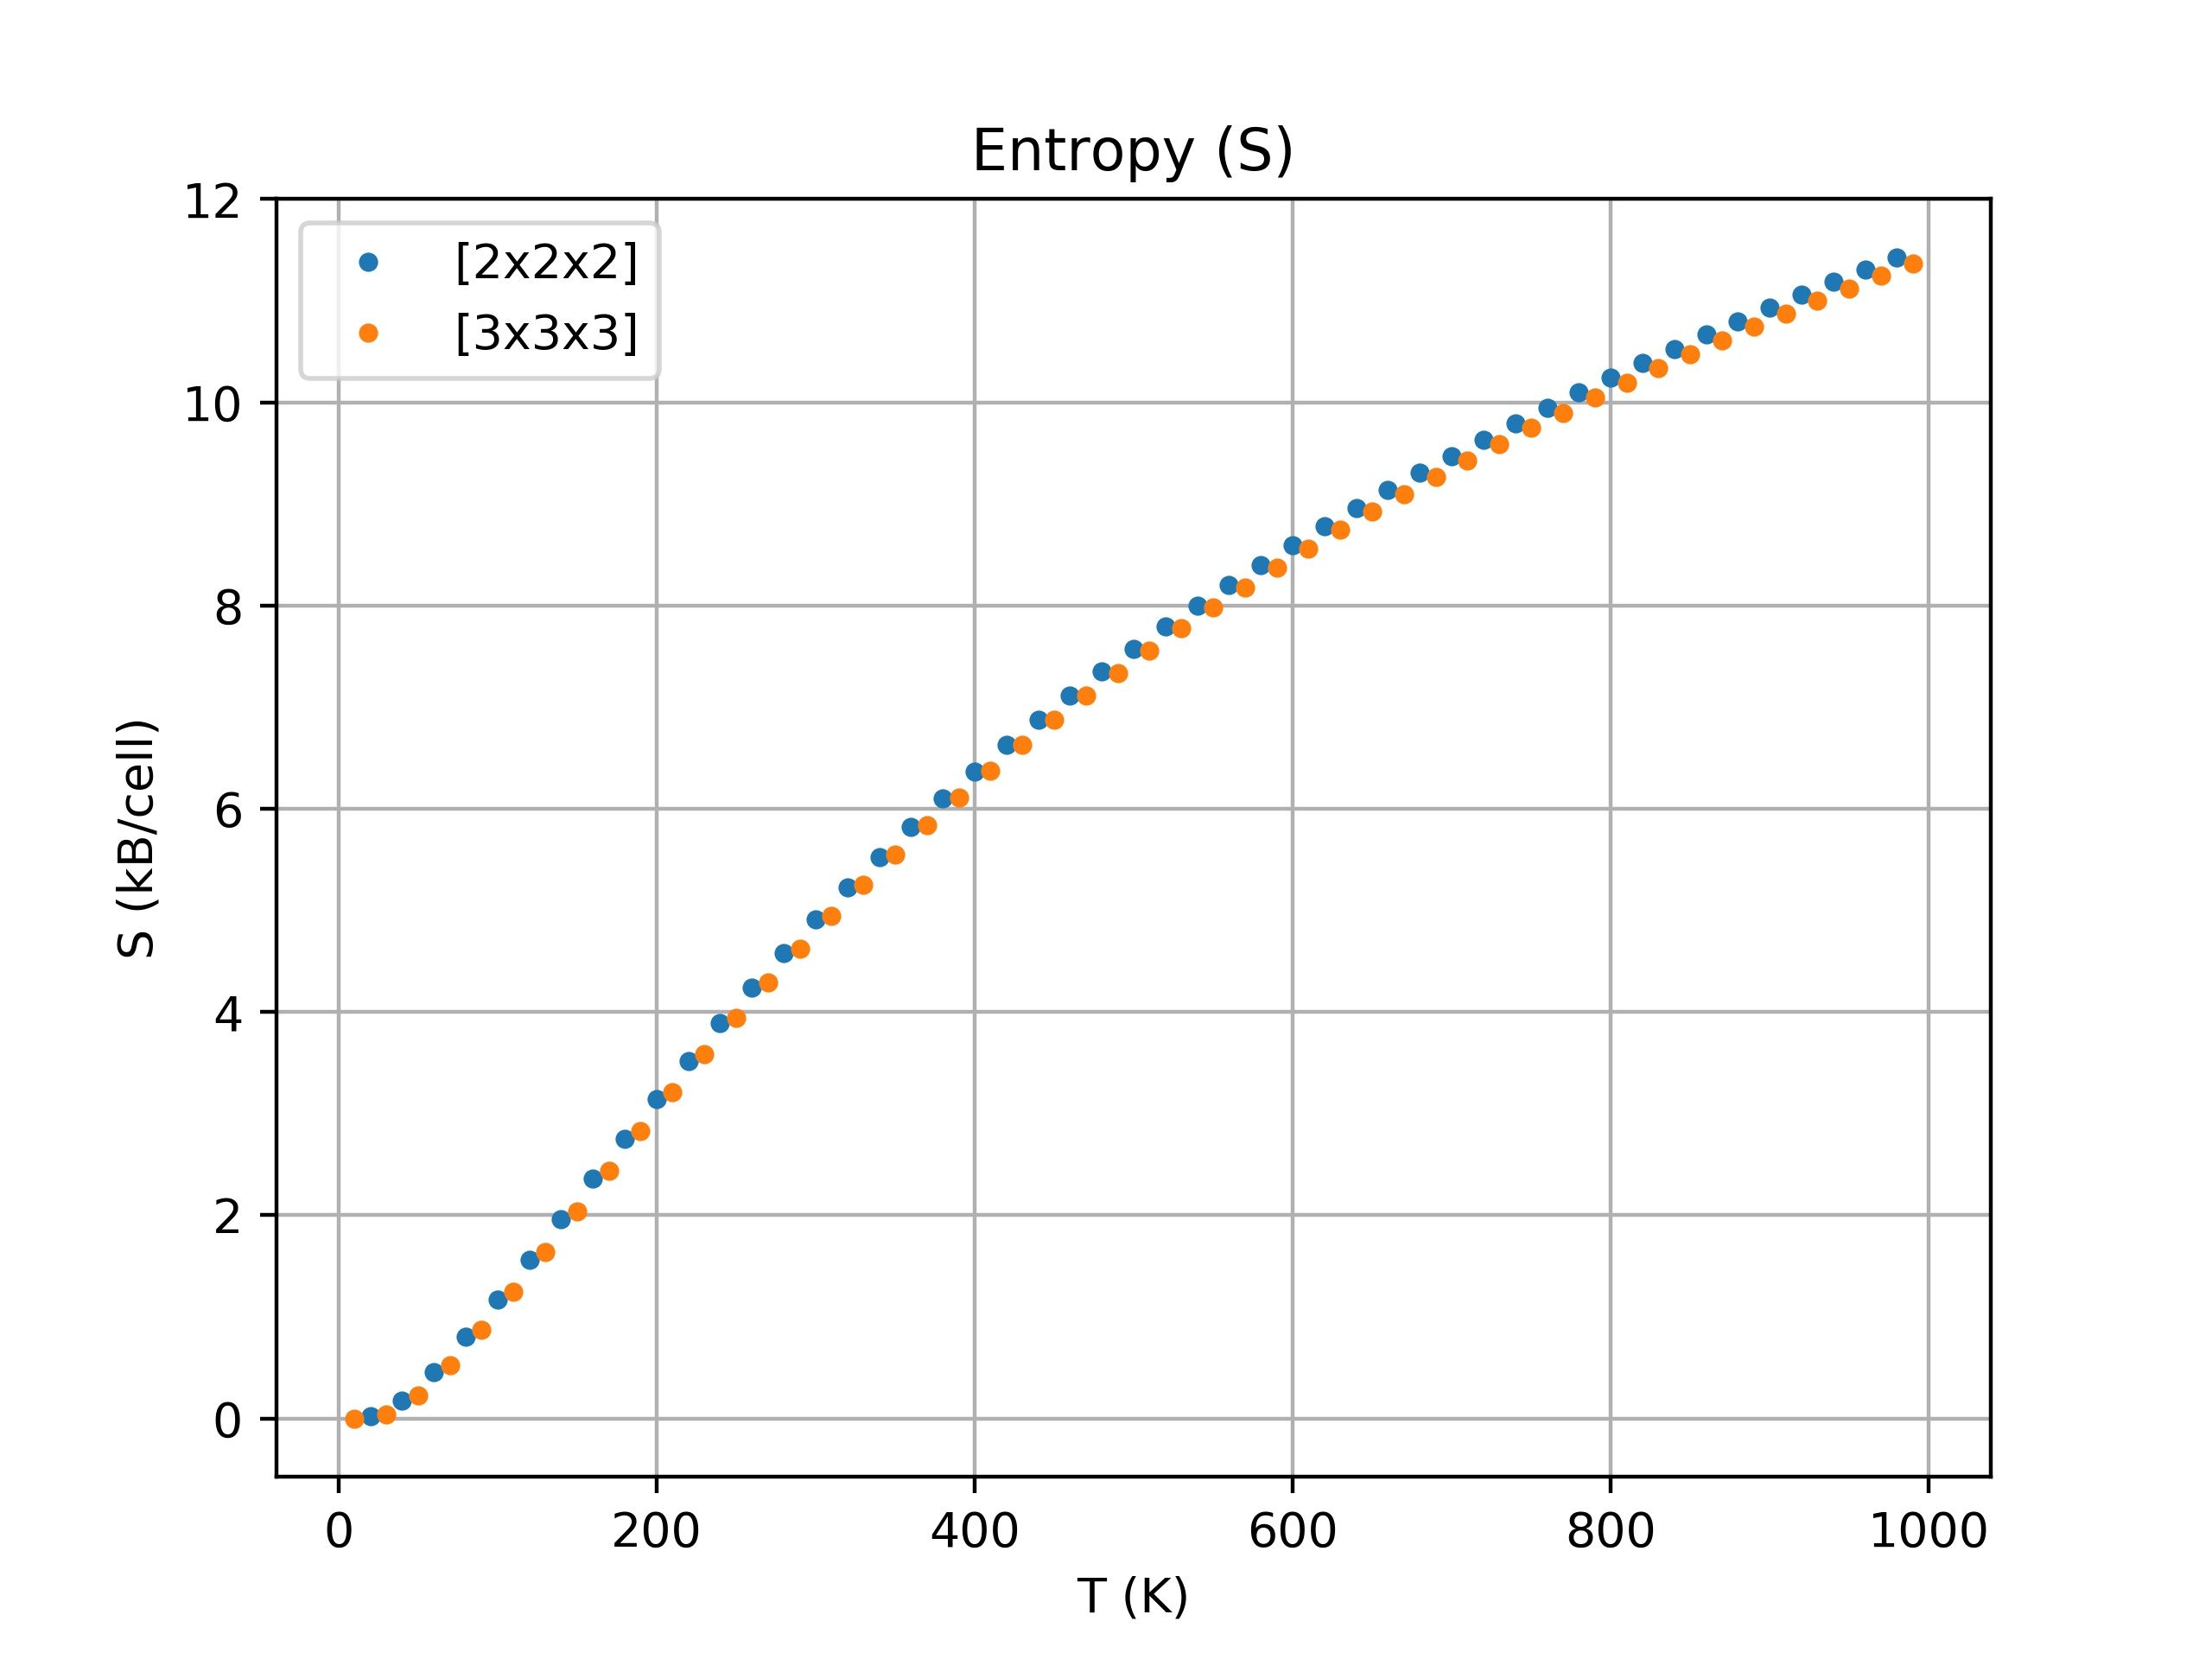
\includegraphics[width=\textwidth]{{data/q3/Si_S}.jpg}
				\caption{Si entropy}
				\label{fig:SiS}
			\end{minipage}
			\begin{minipage}[b]{0.45\textwidth}
				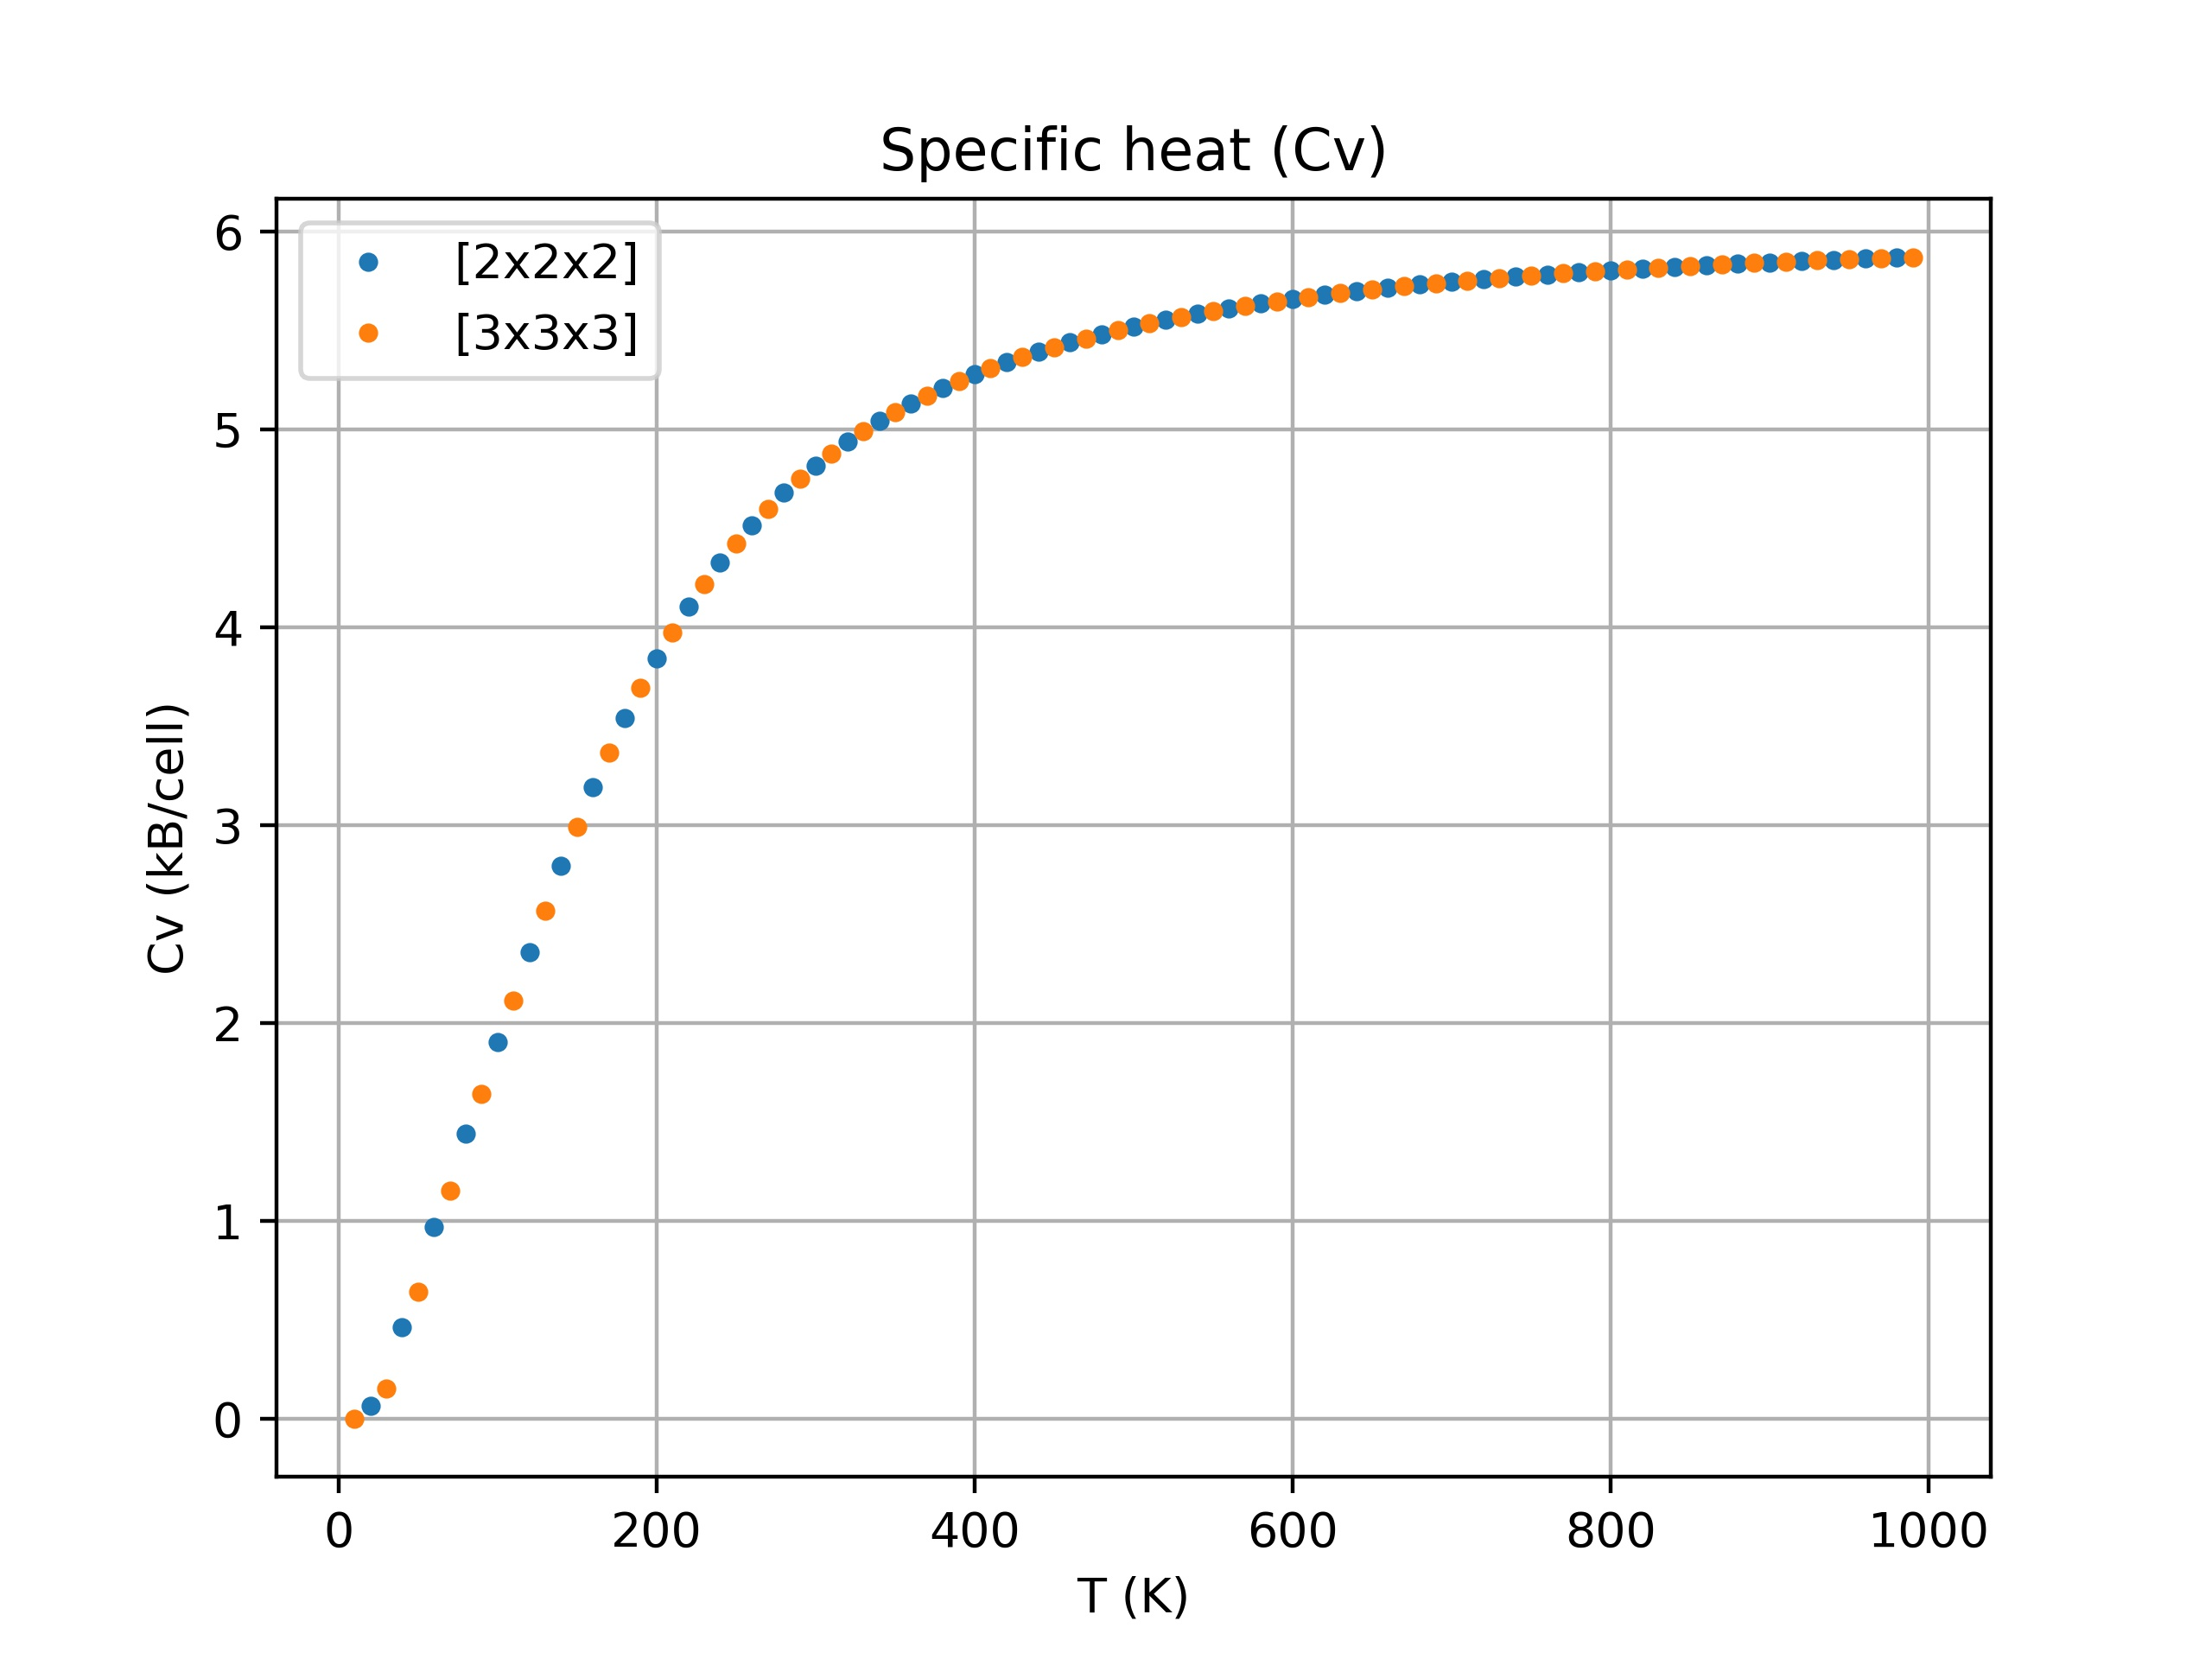
\includegraphics[width=\textwidth]{{data/q3/Si_Cv}.jpg}
				\caption{Si specific heat}
				\label{fig:SiCv}
			\end{minipage}
		\end{figure} 				
		
	\end{enumerate} 
	
	
	% q4: 	
	\item Compute coupling constant J and transition temperature for Mn bcc.
	\begin{enumerate}[label=(\alph*)]
		\item for lattice constant a = 2.89 \AA , the calculated energy for FM and AM states:
		\begin{align*}
			E_{FM} &= -17.5978200 \hspace{0.1cm} (eV) \\
			E_{AM} &= -17.4800880 \hspace{0.1cm} (eV)
		\end{align*}
		
		\item The coupling constant $J$ can be calculated with results in (a) with relation :
		\begin{align*}
			E_{FM} &= E_{PM} + 8J \\
			E_{AF} &= E_{PM} - 8J 
		\end{align*} 
		\begin{align*}
			J &= \left( E_{FM} - E_{AF} \right) / 16 \\
			  &= -0.0073583 \hspace{0.1cm} (eV)
		\end{align*}
		Using mean field approximation we can calculate the transition point where $z = 8$ is the number of neighbors and $S = \frac{1}{2}$ is the spin moment:
		\begin{align*}
			k_B T_c &= \frac{zJ}{3} \\
			T_c &= \frac{8J}{3k_B}\\
				&\approx 227.7053 K
		\end{align*} 
		
		\item We refer to \cite{PhysRevB.38.423}, which reported the magnetization of ferromagnetic bcc-Mn for different lattice constant. Compare with calculation result with $a = 2.89 \AA$:
		\begin{align*}
			m_{ref} &= 0.97   (\mu_B)\\
			m_{cal} &= 1.0198 (\mu_B)
 		\end{align*}
		
		We see that the result are consist with calculation done in\cite{PhysRevB.38.423} 
		
		
		
	
	\end{enumerate}

\end{enumerate}


\end{CJK}

\bibliographystyle{apsrev4-1}
\bibliography{ref}
	

\end{document}

